\documentclass{article}
\usepackage{multicol}
\usepackage{listings}
\usepackage[margin=1in]{geometry}
\usepackage{graphicx}
\usepackage{float}
\usepackage{subcaption}
\newcommand*{\Scale}[2][4]{\scalebox{#1}{$#2$}}
\newcommand*{\Resize}[2]{\resizebox{#1}{!}{$#2$}}
\graphicspath{ {./Figures/} }

\begin{document}

\section{Objectives}
\indent
The objective for this lab is to construct a sequence of shaped pulses and examine the role of pulse shape on intersymbol interference and the effect of noise.

\noindent
During this lab we will look at 4 difference types of line code:
  \begin{itemize}
    \item Polar
    \item On-Off
    \item Bipolar
    \item Differential
  \end{itemize}

\section{Procedure}
\indent
For this lab we designed the system seen in Figure \ref{fig:Full-System}.
There are four specific subsystems that are used. The first is seen in Figure \ref{fig:Polar-System}. This system takes the input of an On-Off Binary signal and generates a Polar signal that goes from negative one to one. This is done with a lookup table where zero corresponds to negative one and one corresponds to one. The second subsystem is seen in Figure \ref{fig:Bipolar-System}. In this subsystem, a running sum is used to keep track of if we are on an odd or even one, uses a look up table to correspond odd ones to a value of one and even ones to correspond to a value of negative one and then uses a multiplier to keep zeros as zeros. The third and final encoder subsystem is one for the differential line code. This is seen in Figure \ref{fig:Duobinary-System} and uses a running sum and lookup table to take the binary input and output a differential line code. The last subsystem just contains a Eye Diagram and Spectrum Analyzer.
\begin{figure}[H]
  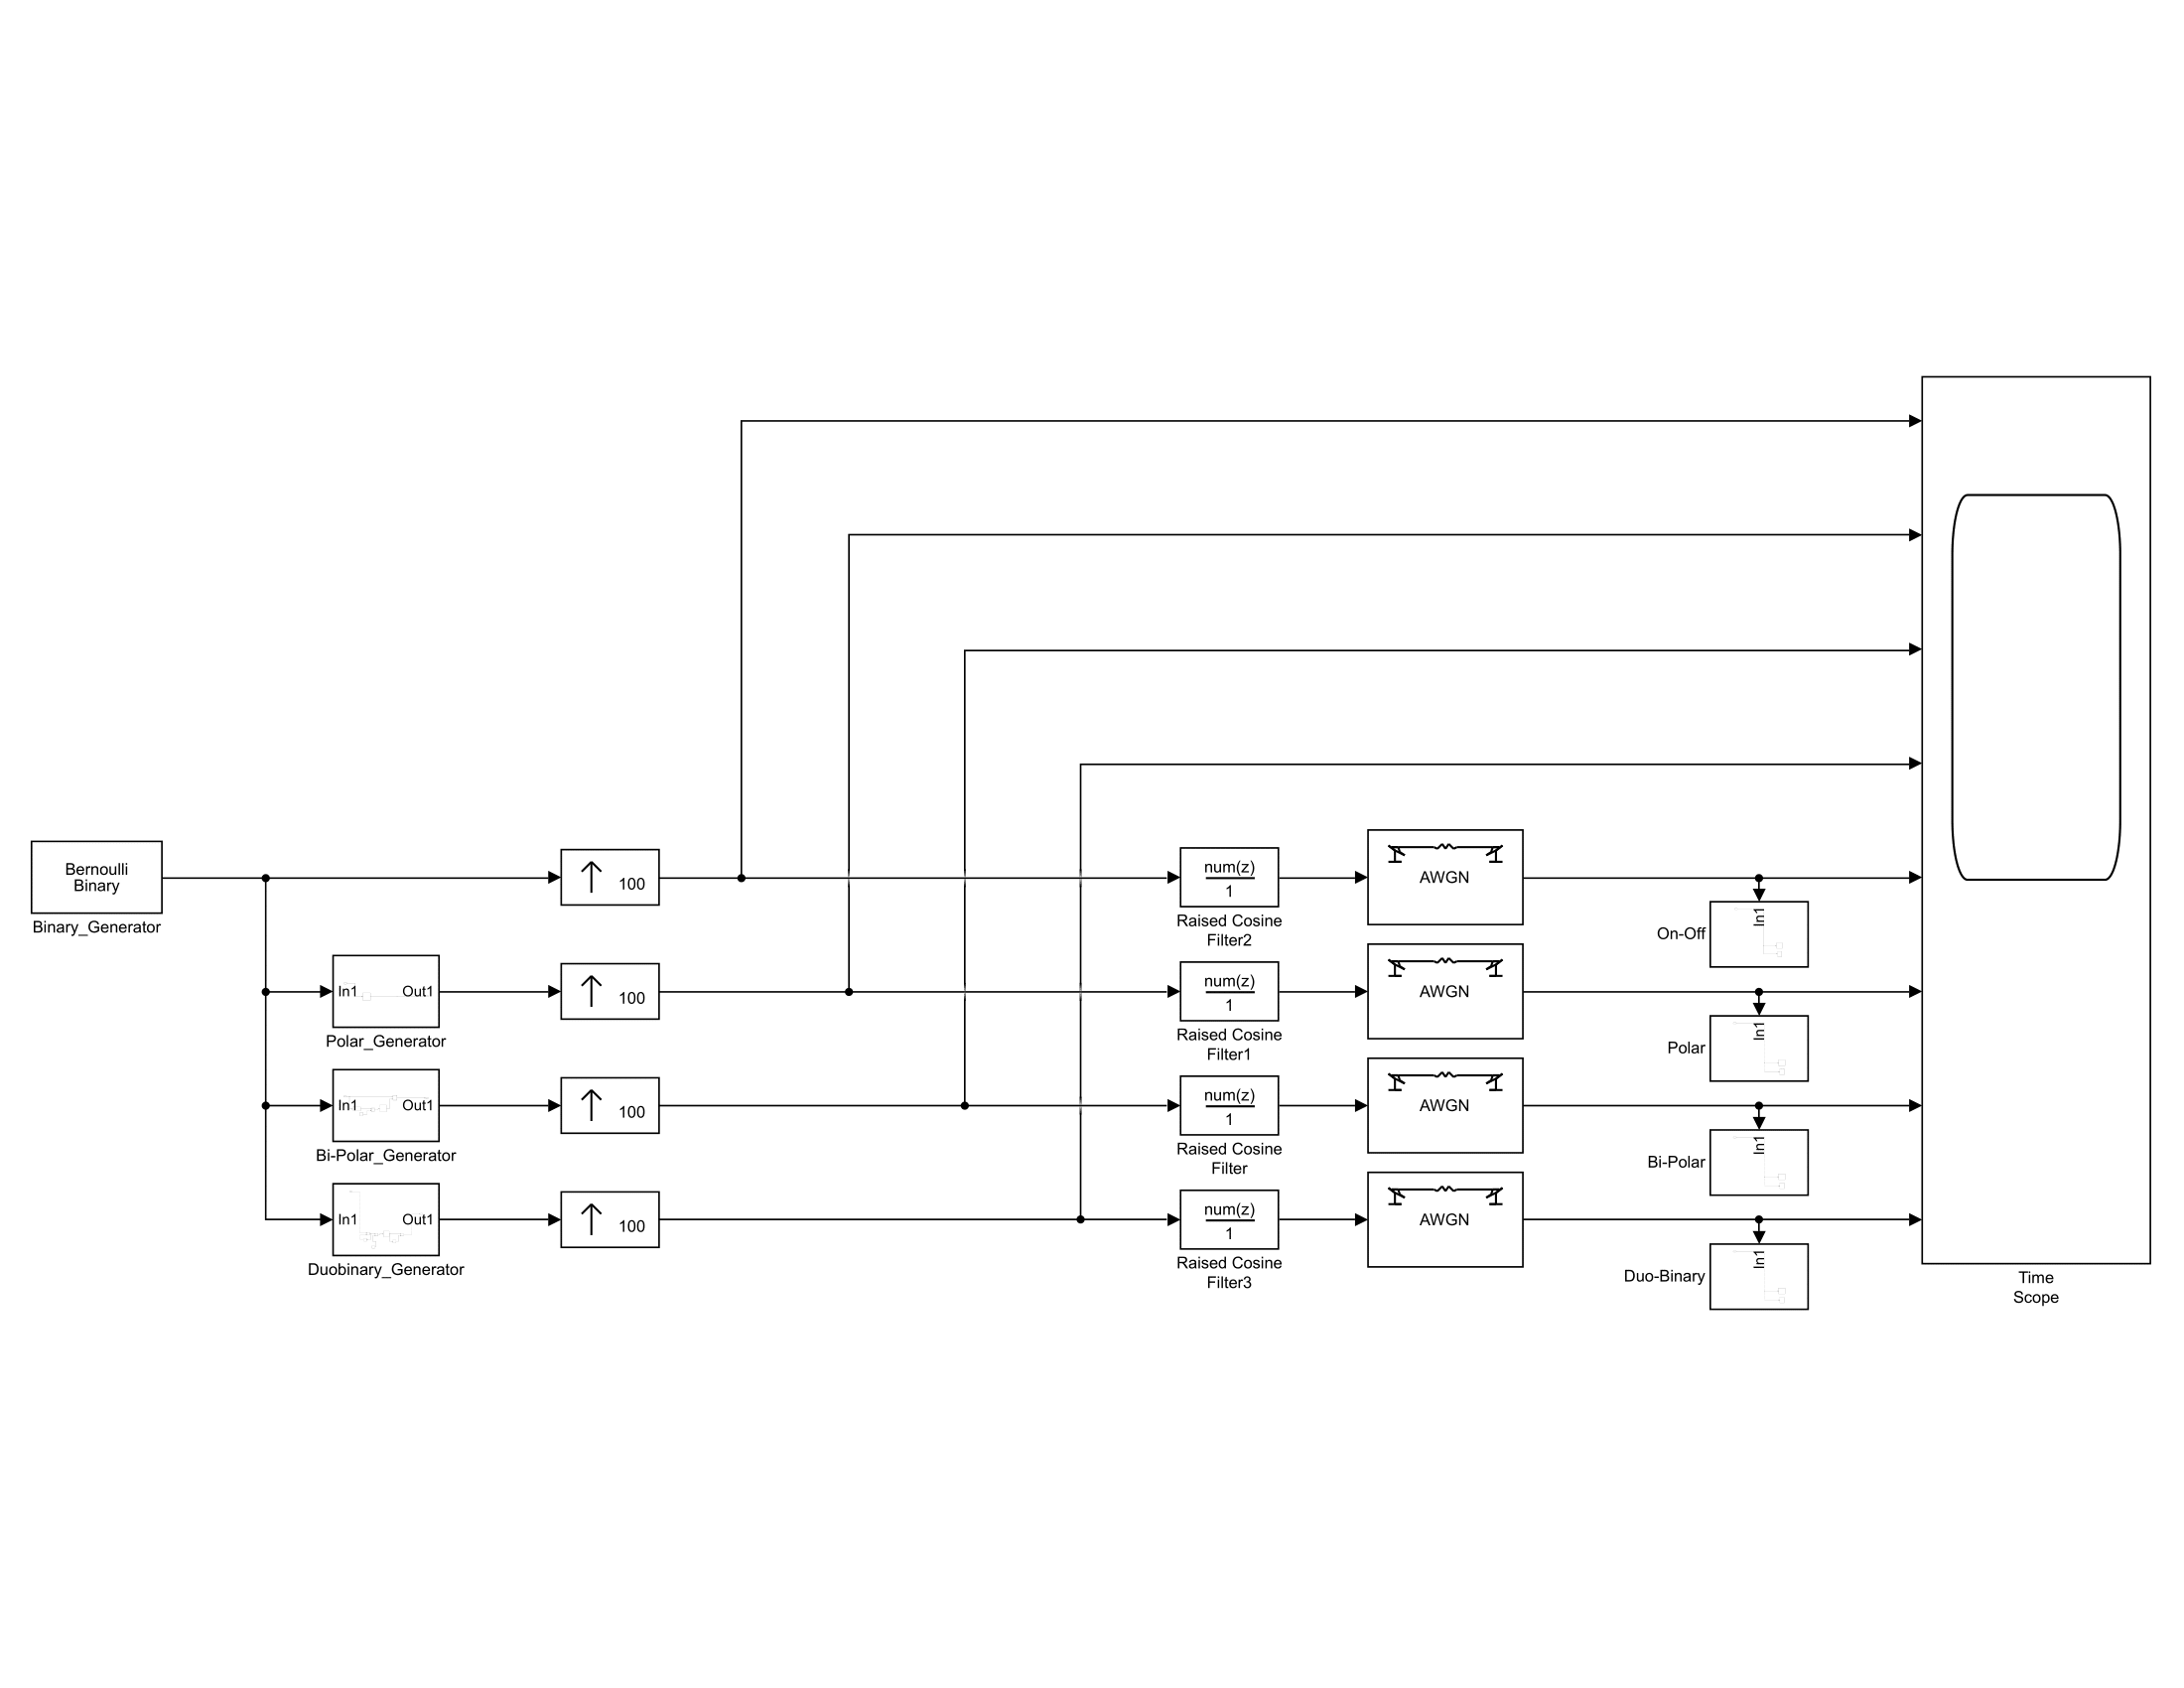
\includegraphics[width = \linewidth]{Full_System.png}
  \caption{Simulink Program created to work with Line Codes}
  \label{fig:Full-System}
\end{figure}
\begin{figure}[H]
  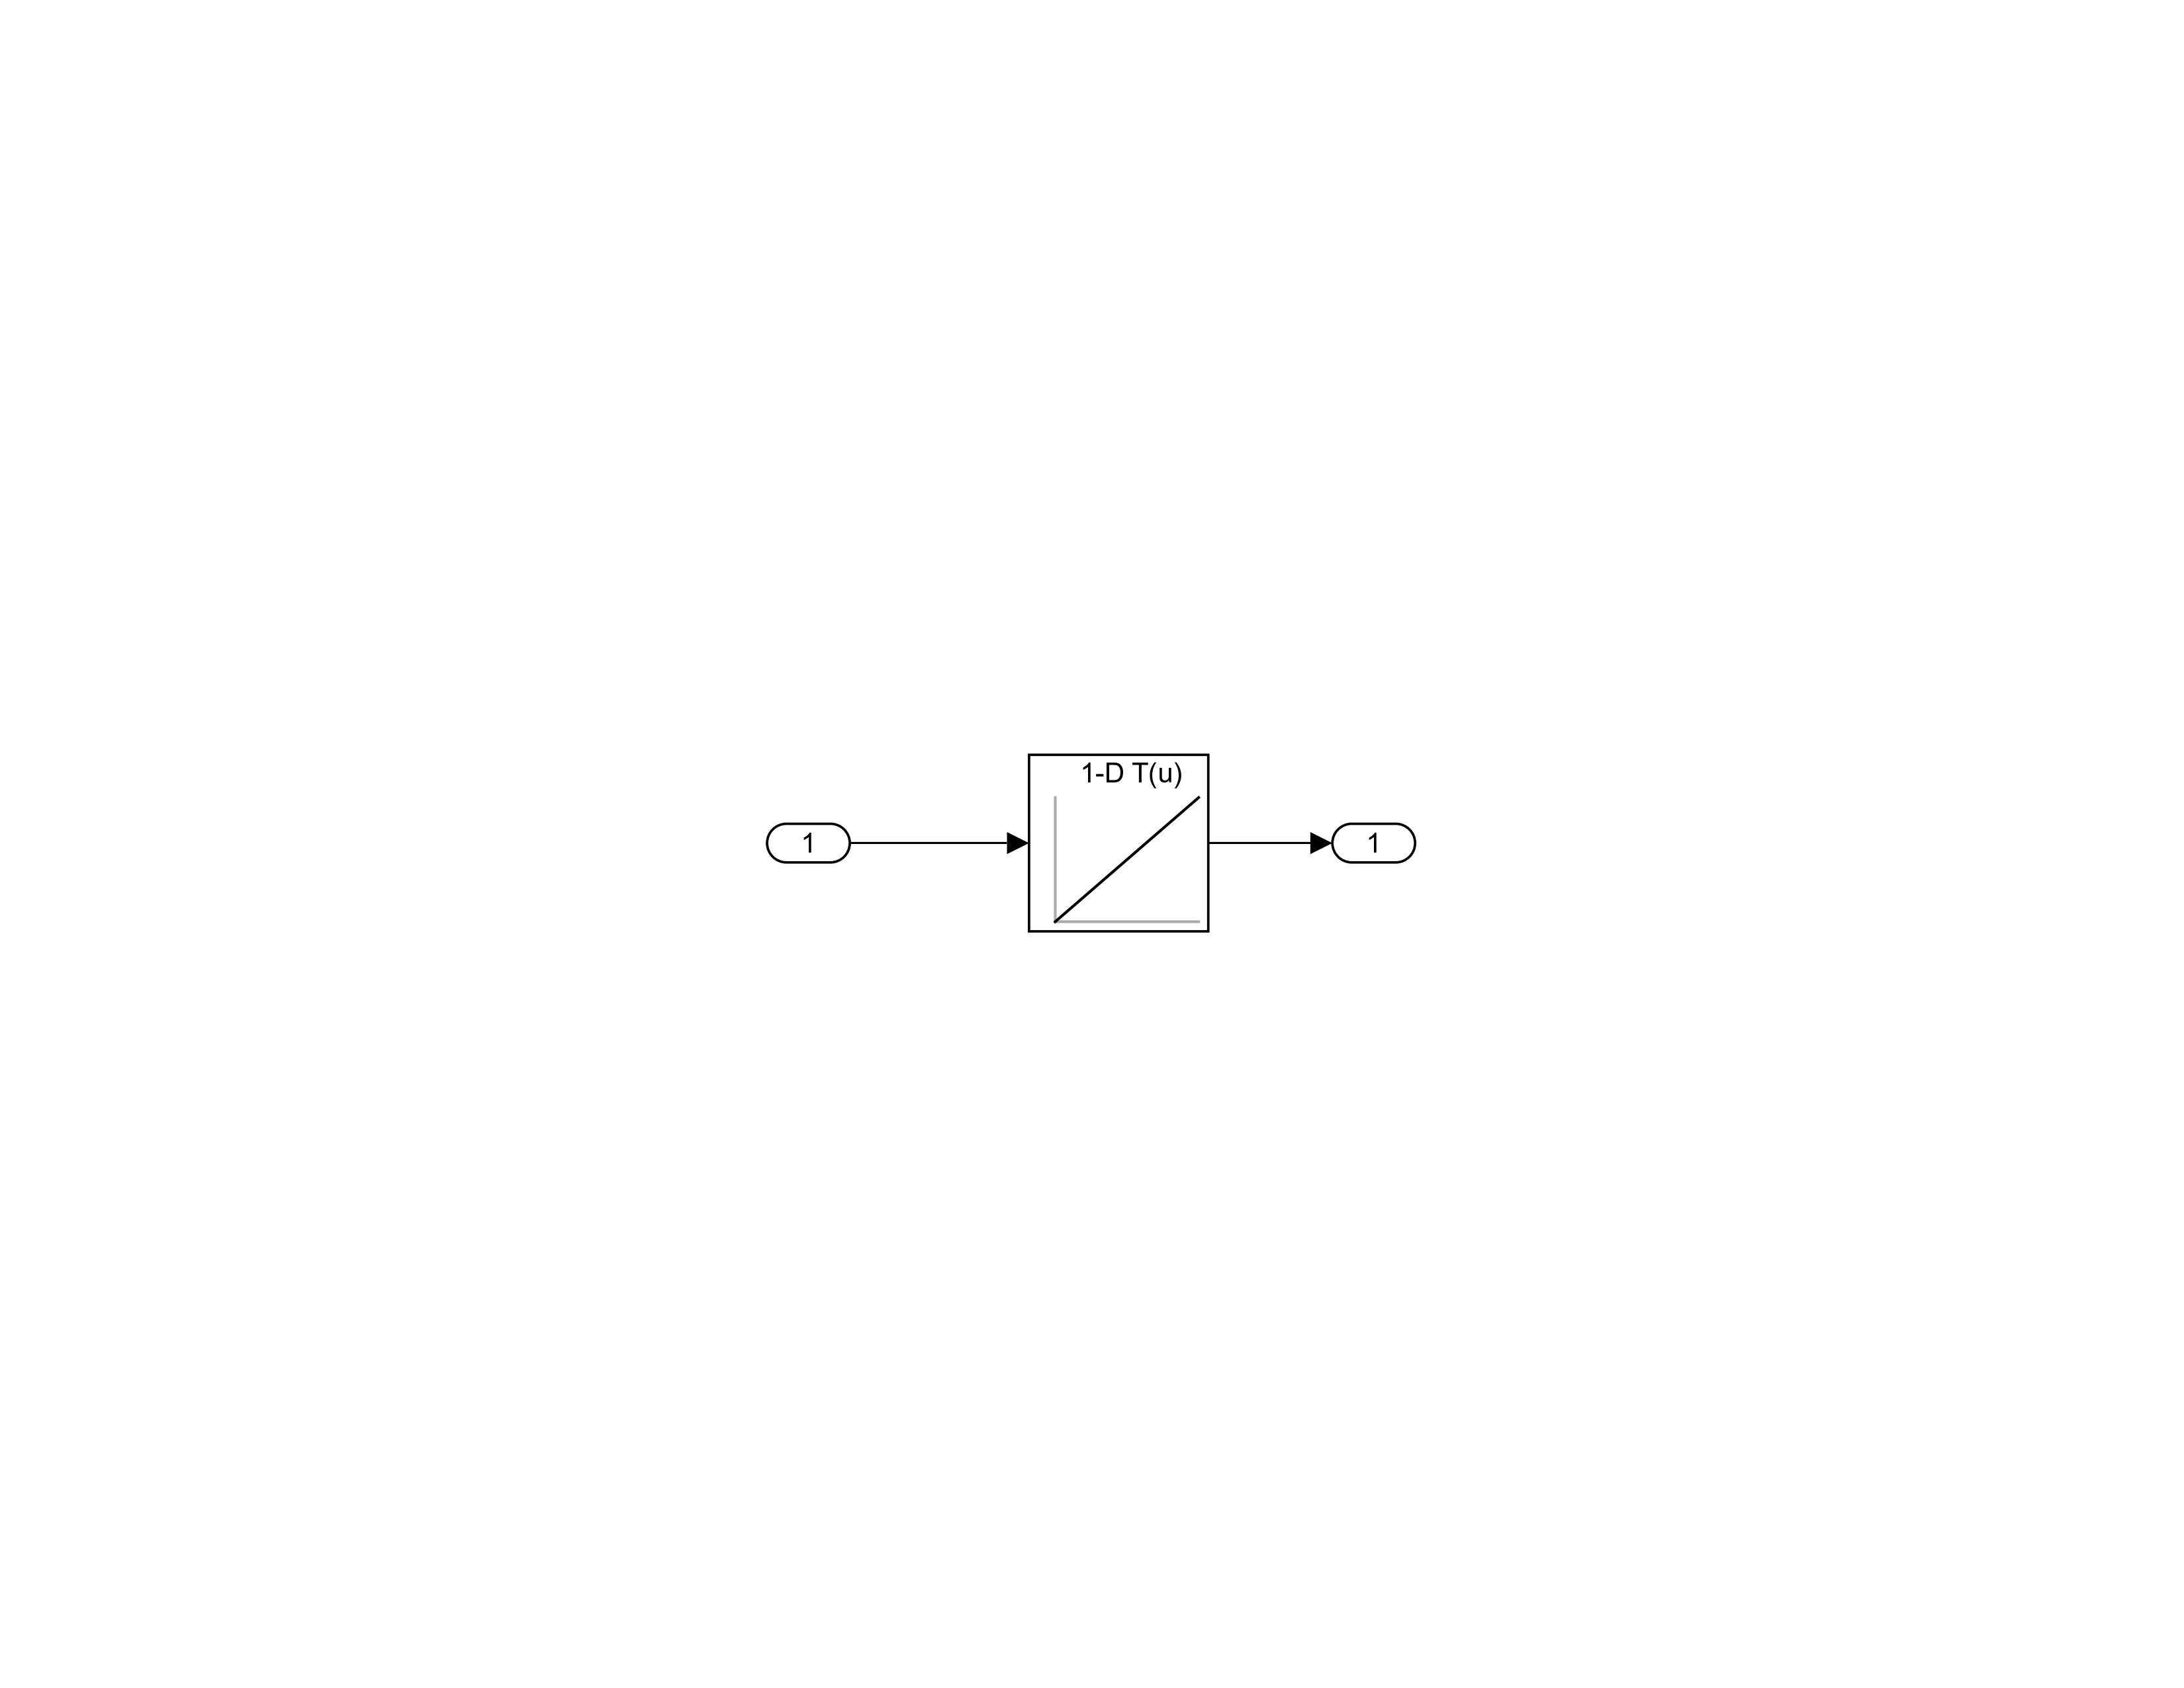
\includegraphics[width = \linewidth]{Polar_Encoder.jpg}
  \caption{Polar Encoder}
  \label{fig:Polar-System}
\end{figure}
\begin{figure}[H]
  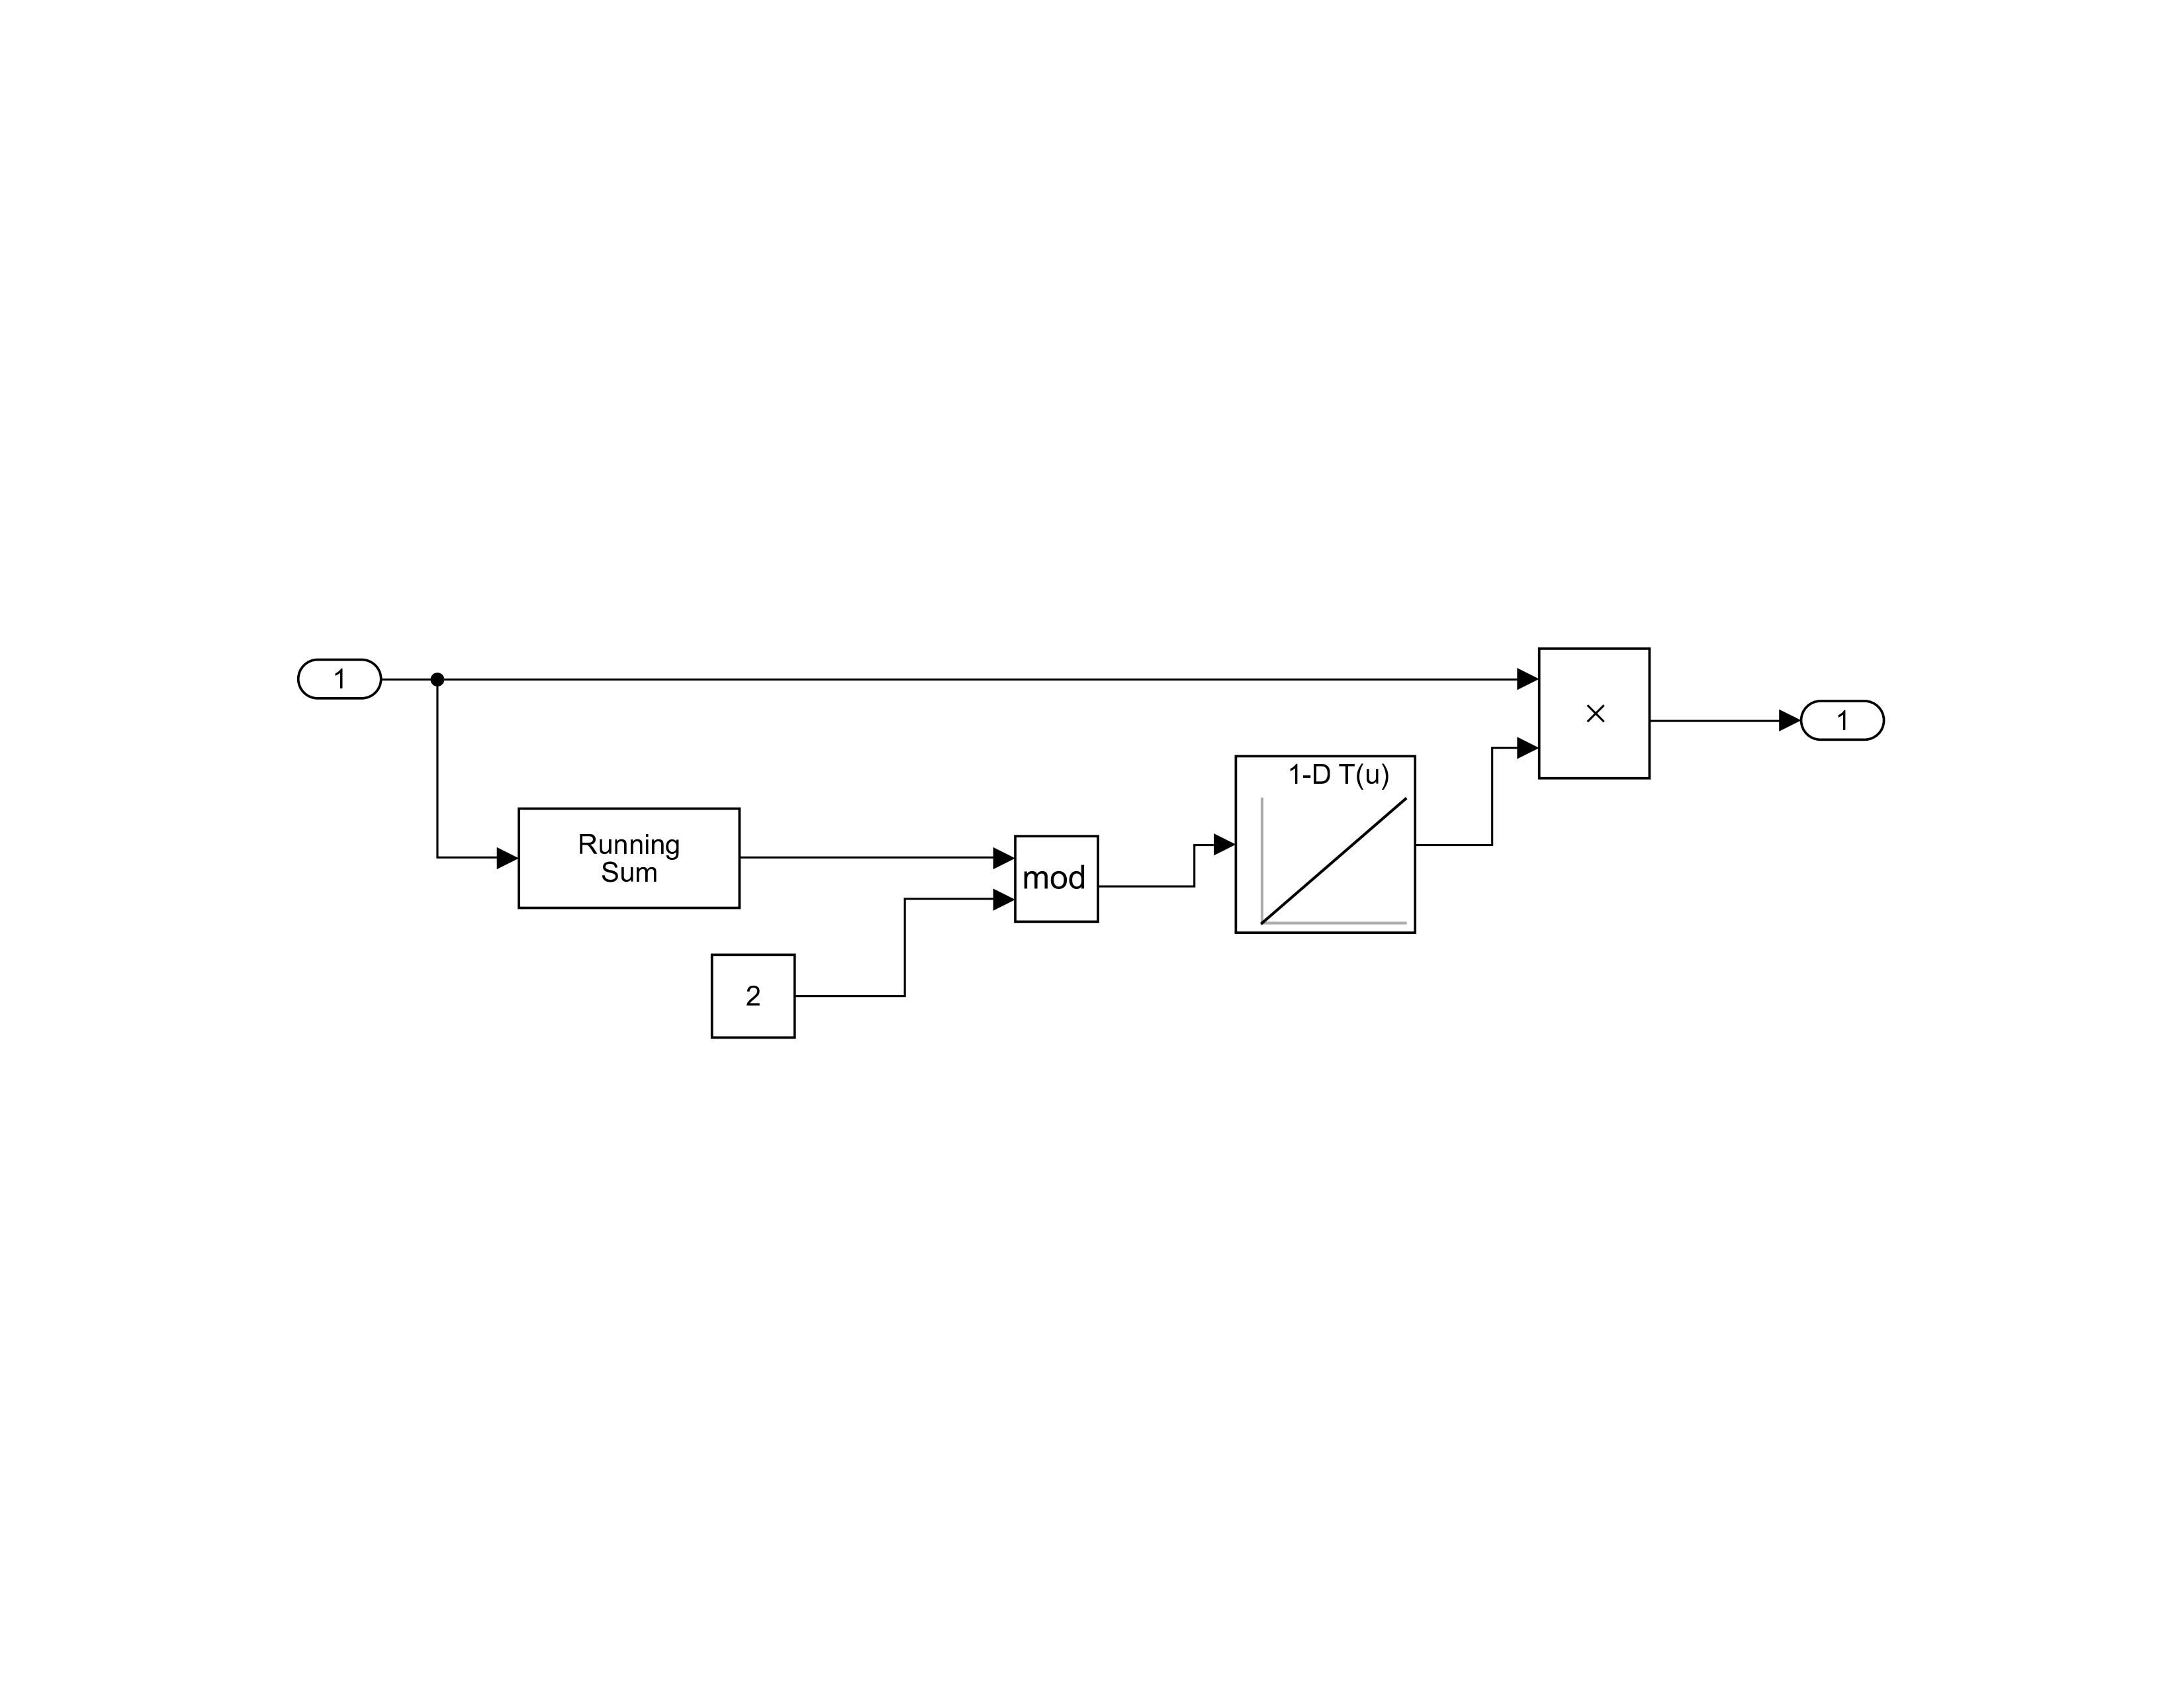
\includegraphics[width = \linewidth]{Bipolar_Encoder.jpg}
  \caption{Bipolar Encoder}
  \label{fig:Bipolar-System}
\end{figure}
\begin{figure}[H]
  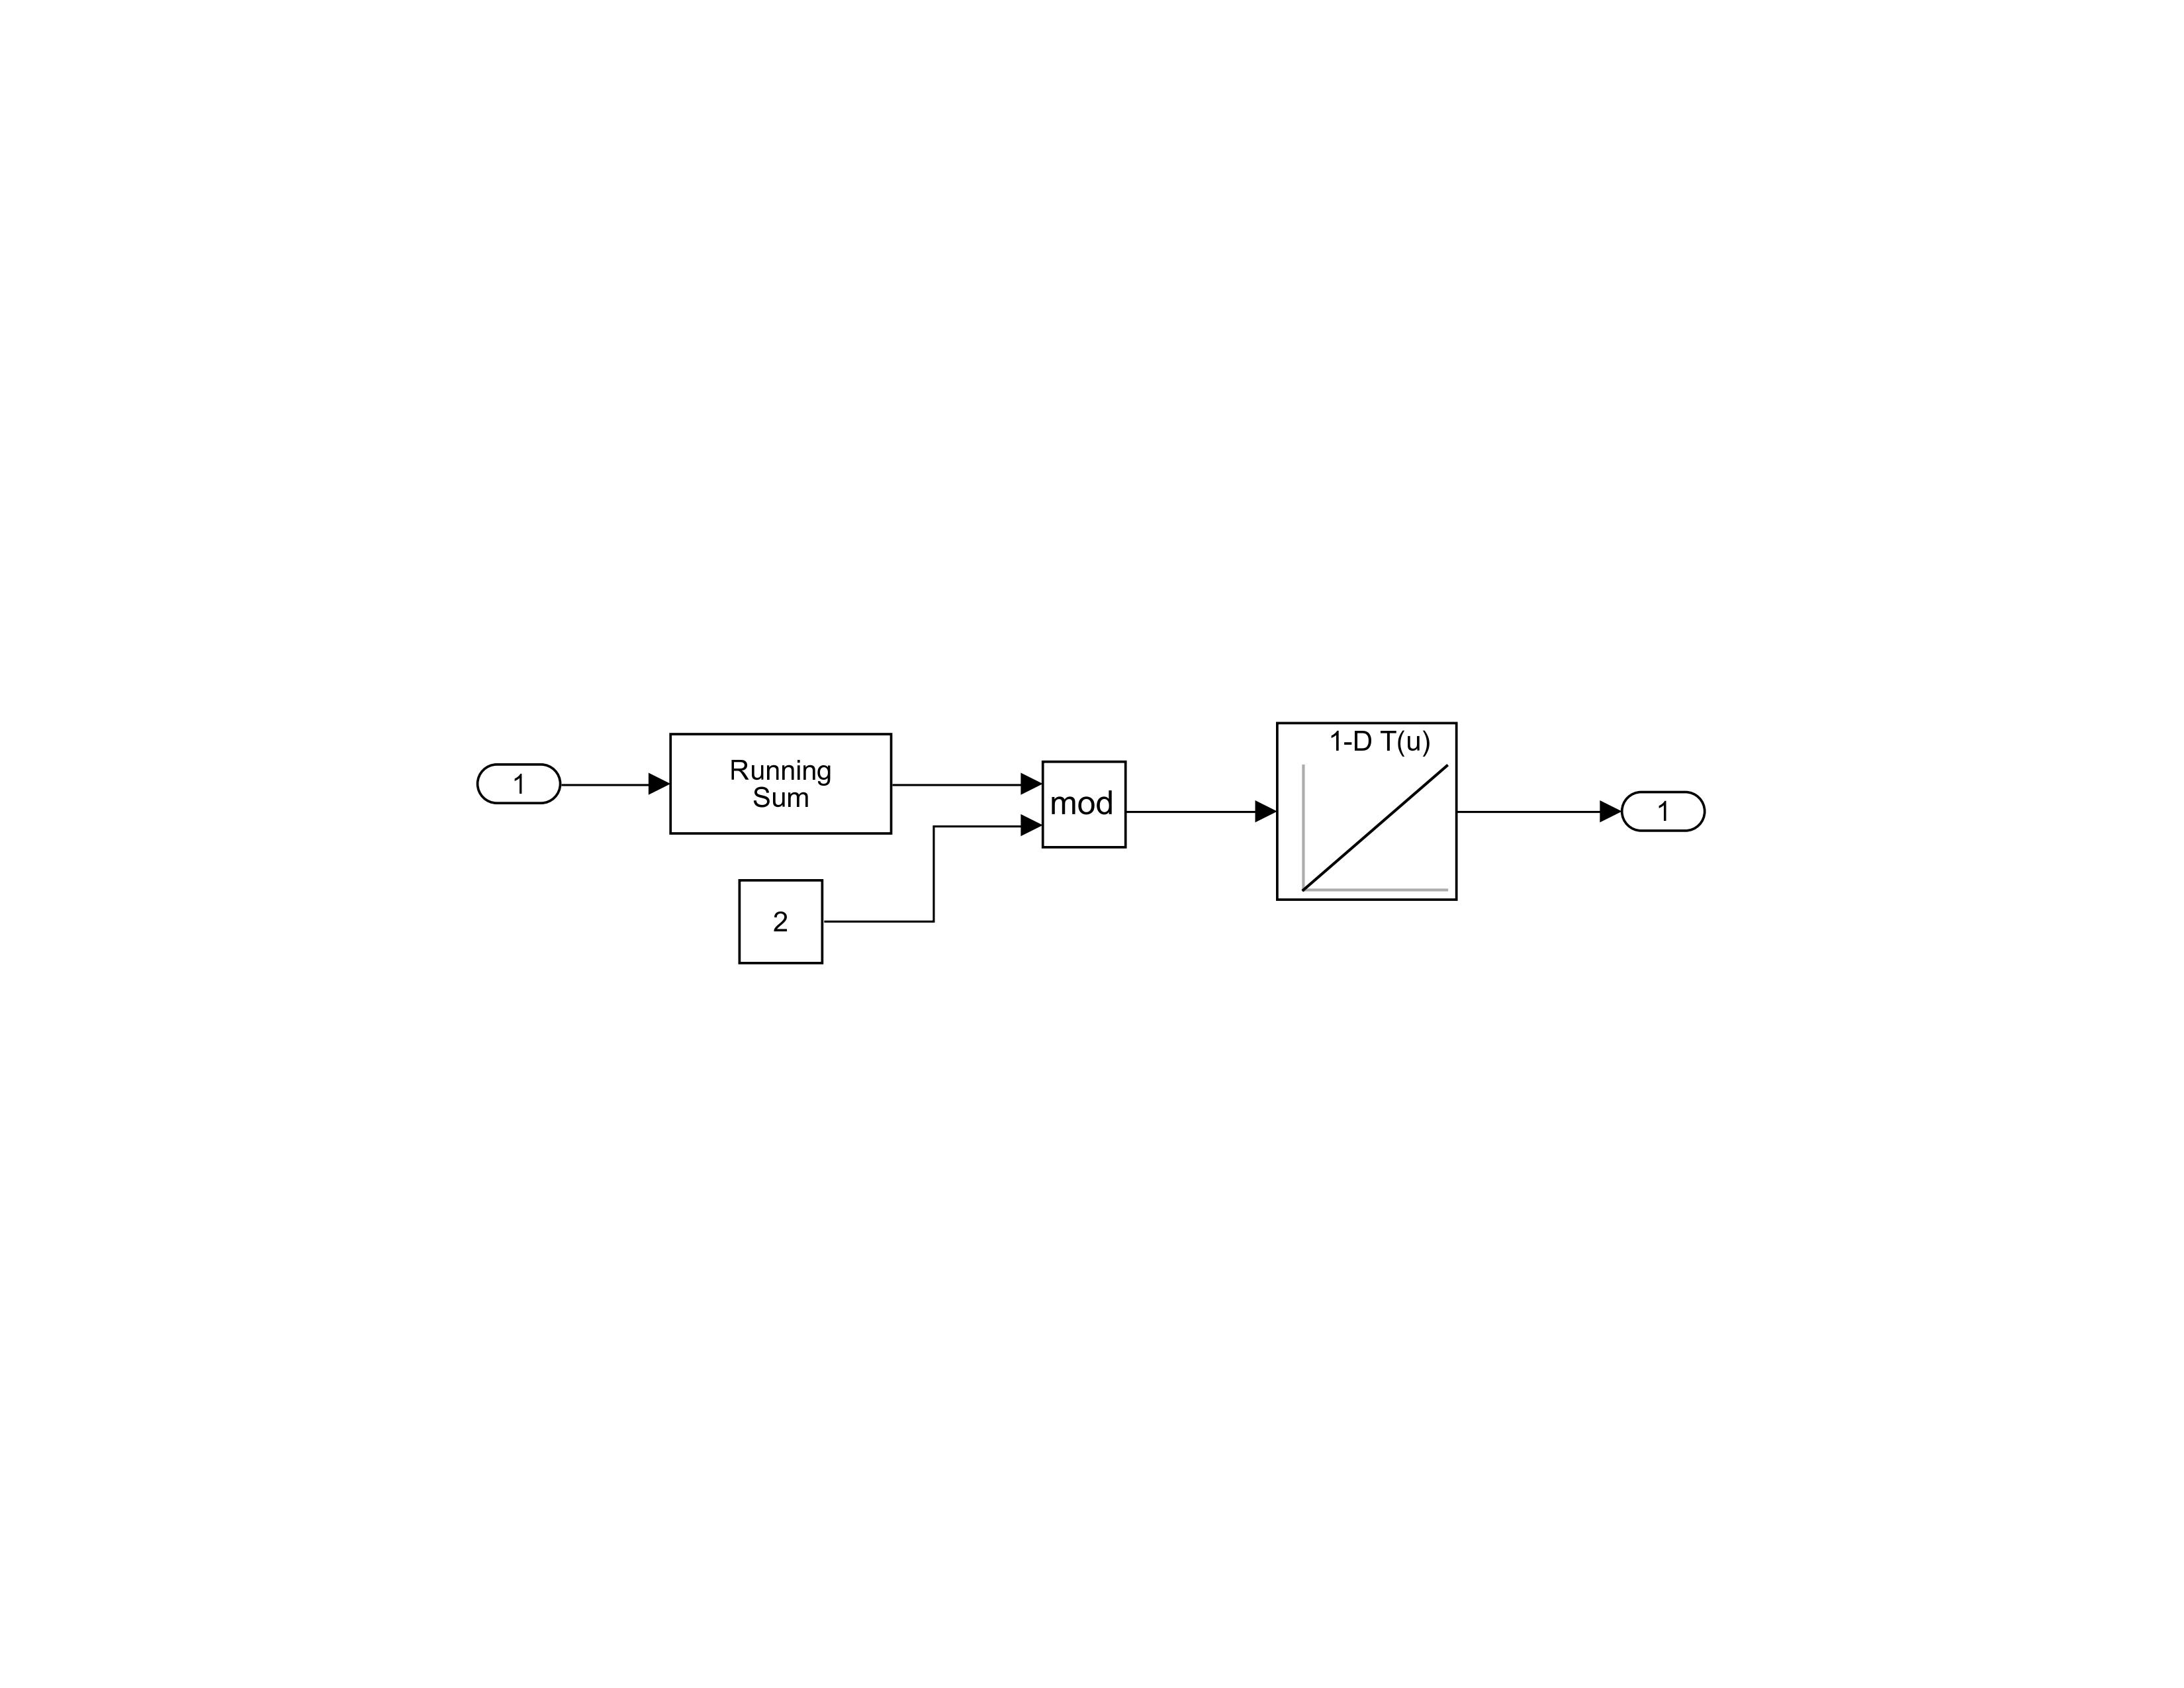
\includegraphics[width = \linewidth]{Differential_Encoder.jpg}
  \caption{Differential Encoder}
  \label{fig:Duobinary-System}
\end{figure}
\subsection{Pulse Types}
During this lab we will be using a variety of pulse shapes. Below are the different pulse shapes that I used.
\subsubsection{Raised Cosine Pulse}
\begin{figure}[H]
  \begin{center}
    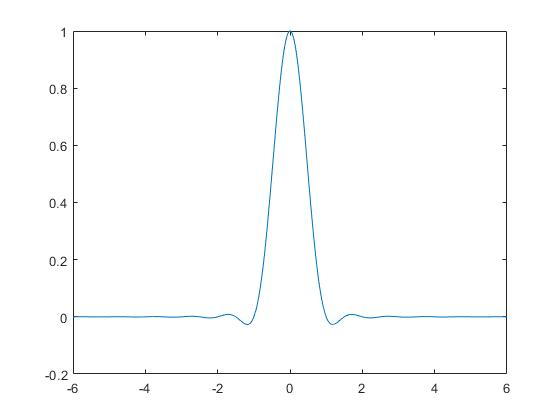
\includegraphics[width = 0.4\linewidth]{Raised_Cosine_Pulse.jpg}
    \caption{Raised Cosine Pulse}
    \label{fig:Raised_Cosine_Pulse}
  \end{center}
\end{figure}
\subsubsection{Triangle Pulse}
\begin{figure}[H]
  \begin{center}
    \begin{subfigure}[b]{0.4\linewidth}
      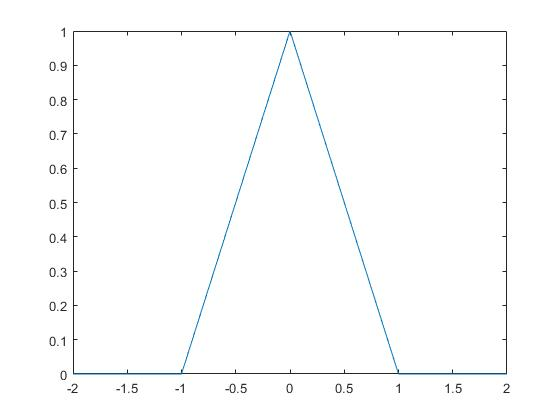
\includegraphics[width = \linewidth]{Tri_Half.jpg}
      \caption{Triangular Half Width Pulse}
    \end{subfigure}
    \begin{subfigure}[b]{0.4\linewidth}
      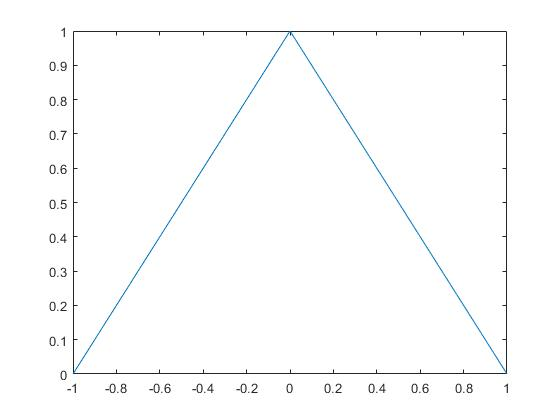
\includegraphics[width = \linewidth]{Tri_Full.jpg}
      \caption{Triangular Full Width Pulse}
    \end{subfigure}
    \caption{Triangular Pulse}
    \label{fig:Tri}
  \end{center}
\end{figure}
\subsubsection{Rectangle Half Width}
\begin{figure}[H]
  \begin{center}
    \begin{subfigure}[b]{0.4\linewidth}
      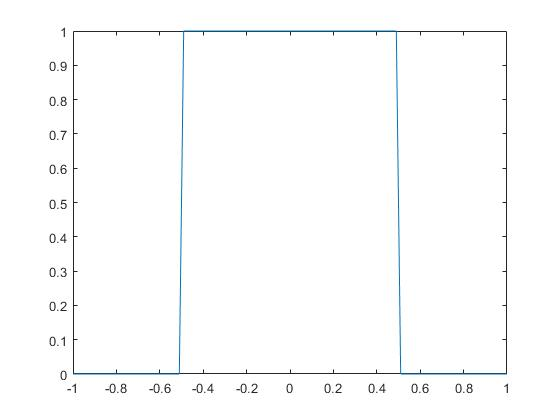
\includegraphics[width = \linewidth]{Rect_Half.jpg}
      \caption{Rectangular Half Width Pulse}
    \end{subfigure}
    \begin{subfigure}[b]{0.4\linewidth}
      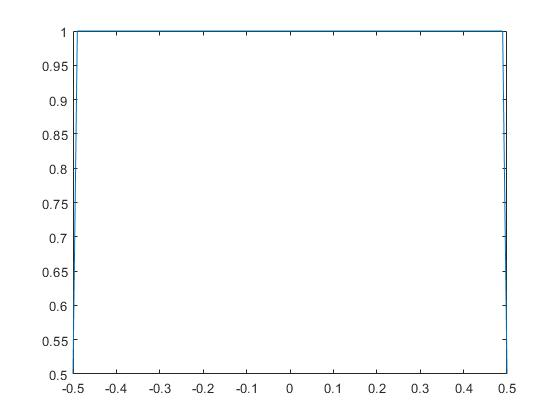
\includegraphics[width = \linewidth]{Rect_Full.jpg}
      \caption{Rectangular Full Width Pulse}
    \end{subfigure}
    \caption{Triangular Pulse}
    \label{fig:Rect}
  \end{center}
\end{figure}
\subsubsection{Sinc}
\begin{figure}[H]
  \begin{center}
    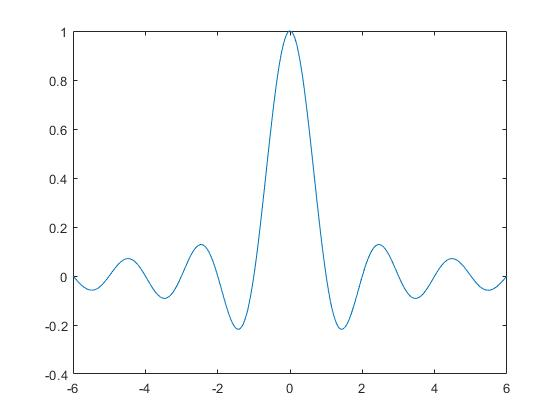
\includegraphics[width = \linewidth]{Sinc_Pulse.jpg}
    \caption{Raised Cosine Pulse}
    \label{fig:Sinc-Pulse}
  \end{center}
\end{figure}
\subsubsection{Sinc Squared}
\begin{figure}[H]
  \begin{center}
    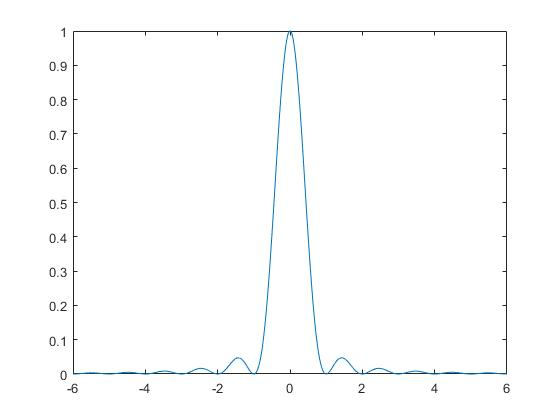
\includegraphics[width = \linewidth]{Sinc_2_Pulse.jpg}
    \caption{Raised Cosine Pulse}
    \label{fig:Sinc-Squared}
  \end{center}
\end{figure}
\subsubsection{Sin Pulse}
\begin{figure}[H]
  \begin{center}
    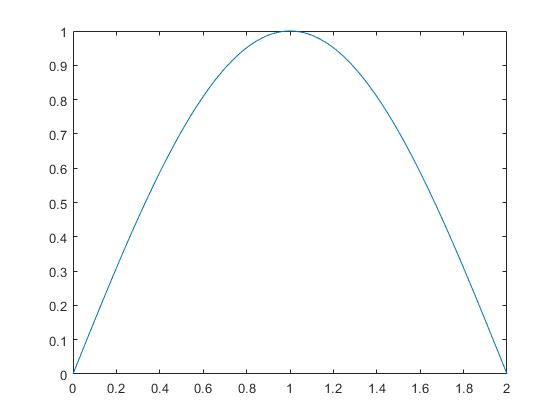
\includegraphics[width = \linewidth]{Sin_Pulse.jpg}
    \caption{Raised Cosine Pulse}
    \label{fig:Sin-Pulse}
  \end{center}
\end{figure}
\section{Results}
\subsection{On-Off}
\subsubsection{Time Signal}
The following images or for On-Off encoding with the various pulse shapes. They
are presented with the On-Off encoded binary stream, the generated signal when
convoluted with a shaped pulse and the received signal with noise in the channel.
\begin{figure}[H]
  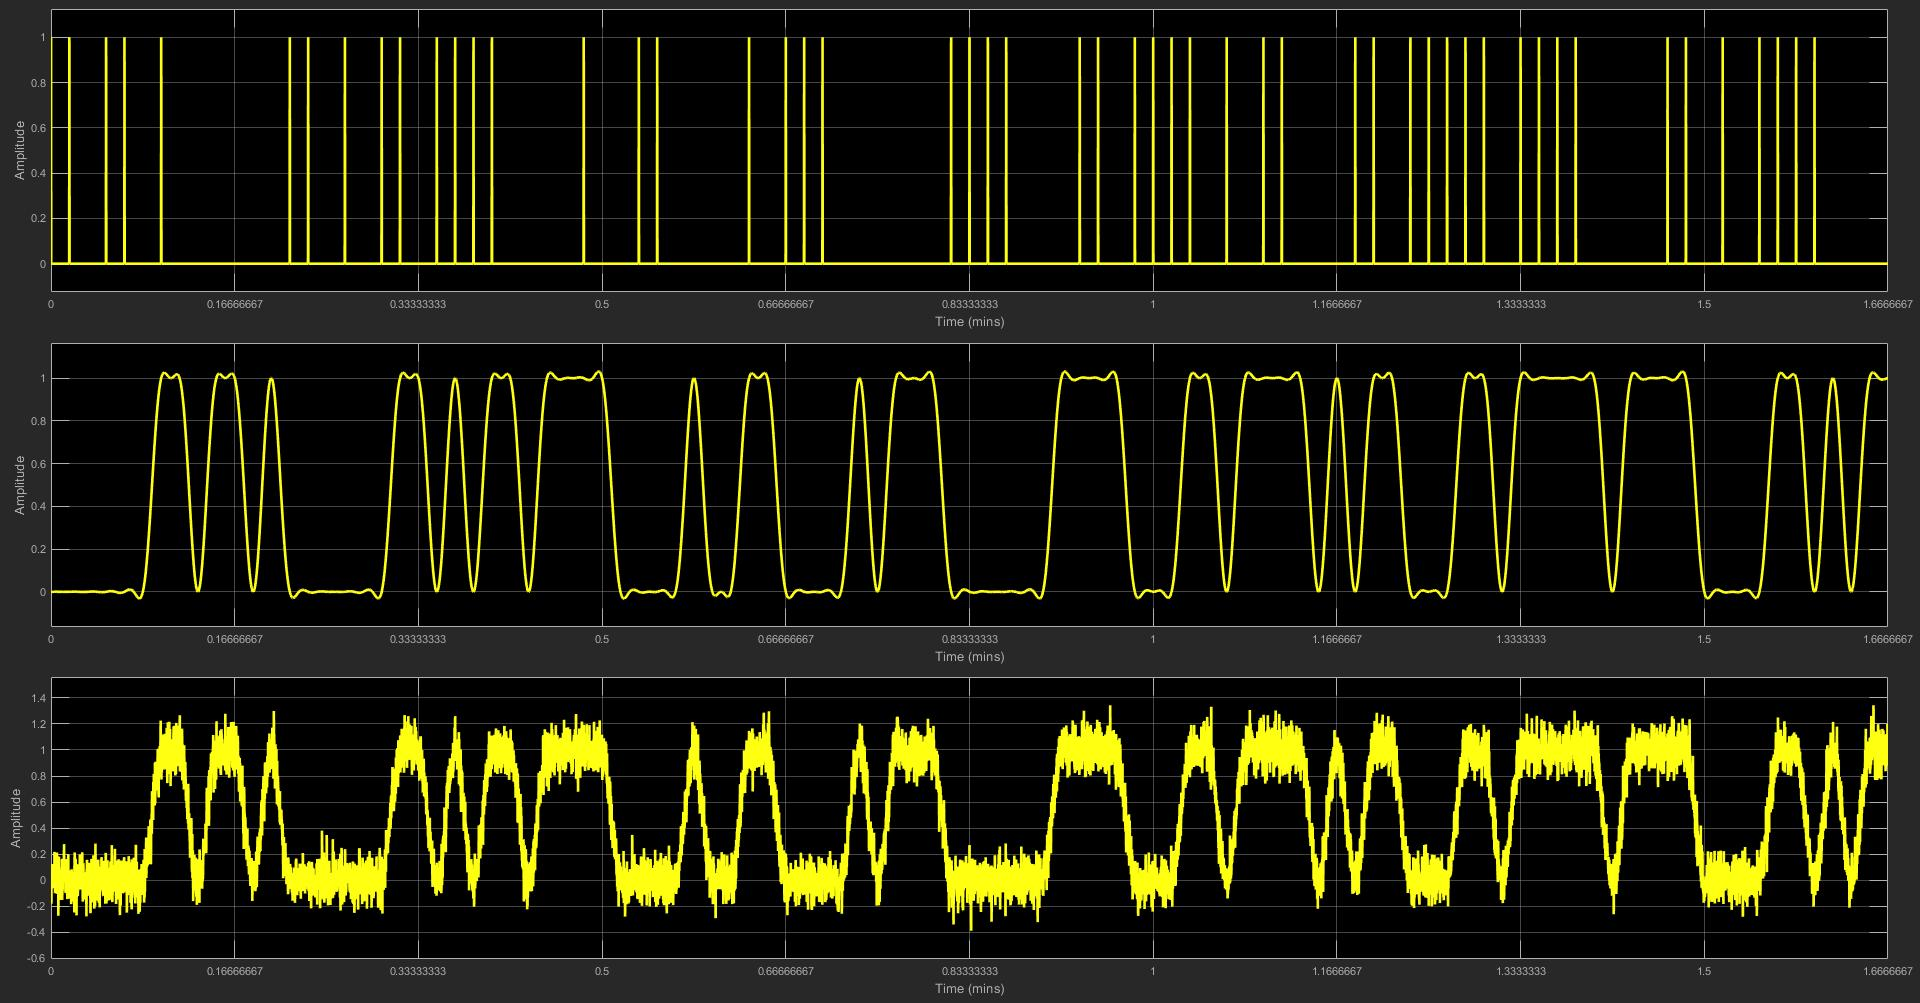
\includegraphics[width = \linewidth]{OO_Rasied.jpg}
  \caption{On-Off encoding with a Raised Cosine Shaped Pulse}
  \label{fig:OO-Raised}
\end{figure}
\begin{figure}[H]
  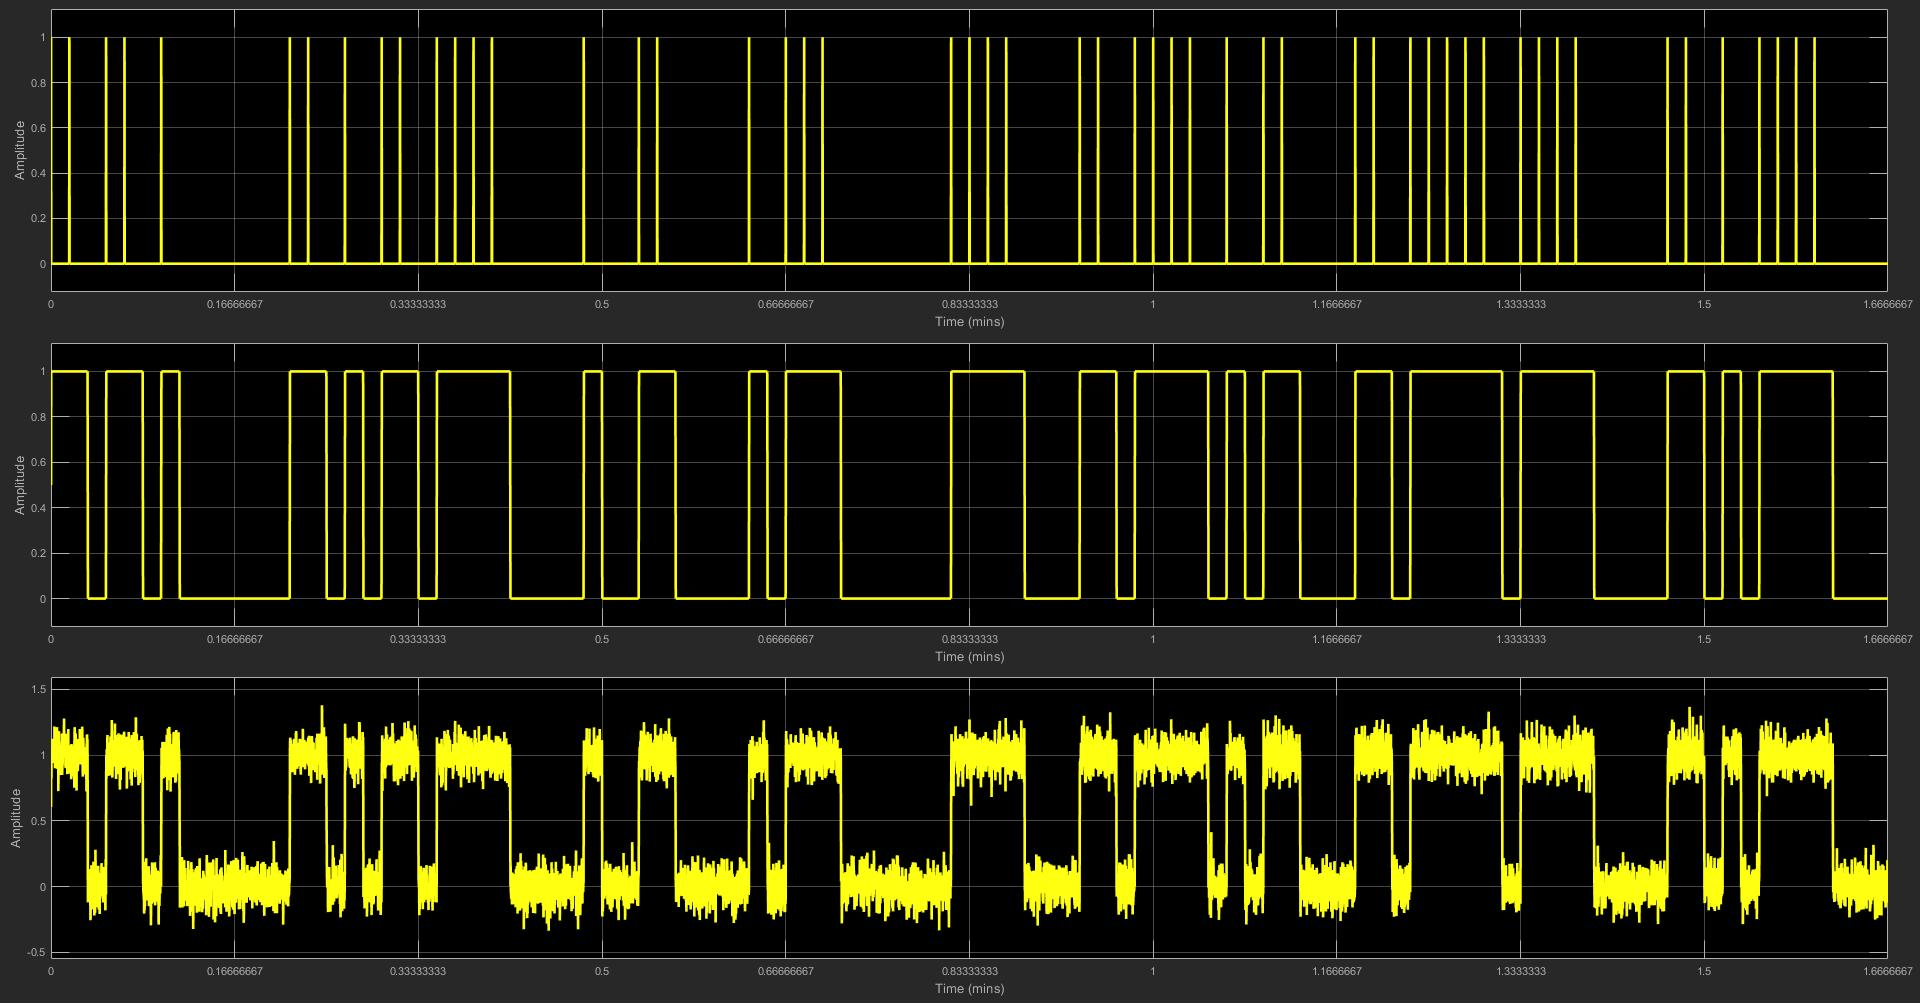
\includegraphics[width = \linewidth]{OO_Rect_F.jpg}
  \caption{On-Off encoding with a Full Width Rectangle Shaped Pulse}
  \label{fig:OO-Rect-F}
\end{figure}
\begin{figure}[H]
  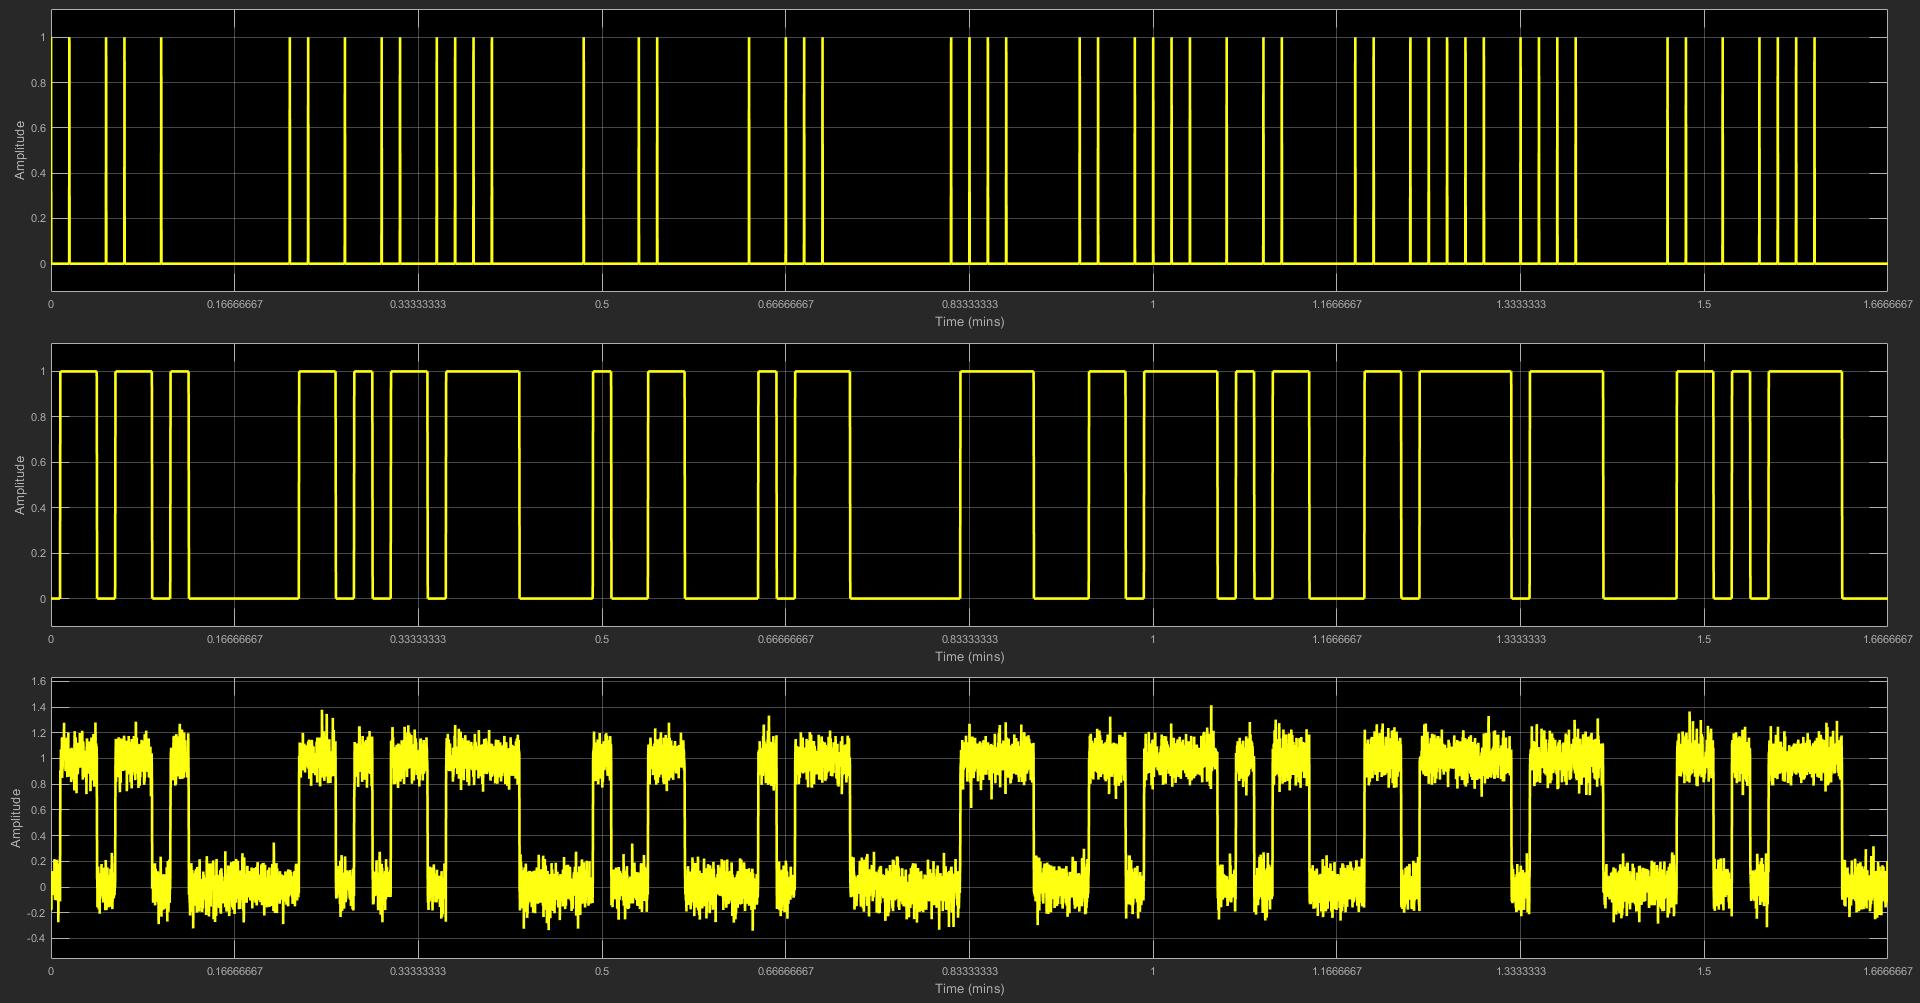
\includegraphics[width = \linewidth]{OO_Rect_H.jpg}
  \caption{On-Off encoding with a Half Width Rectangle Shaped Pulse}
  \label{fig:OO-Rect-H}
\end{figure}
\begin{figure}[H]
  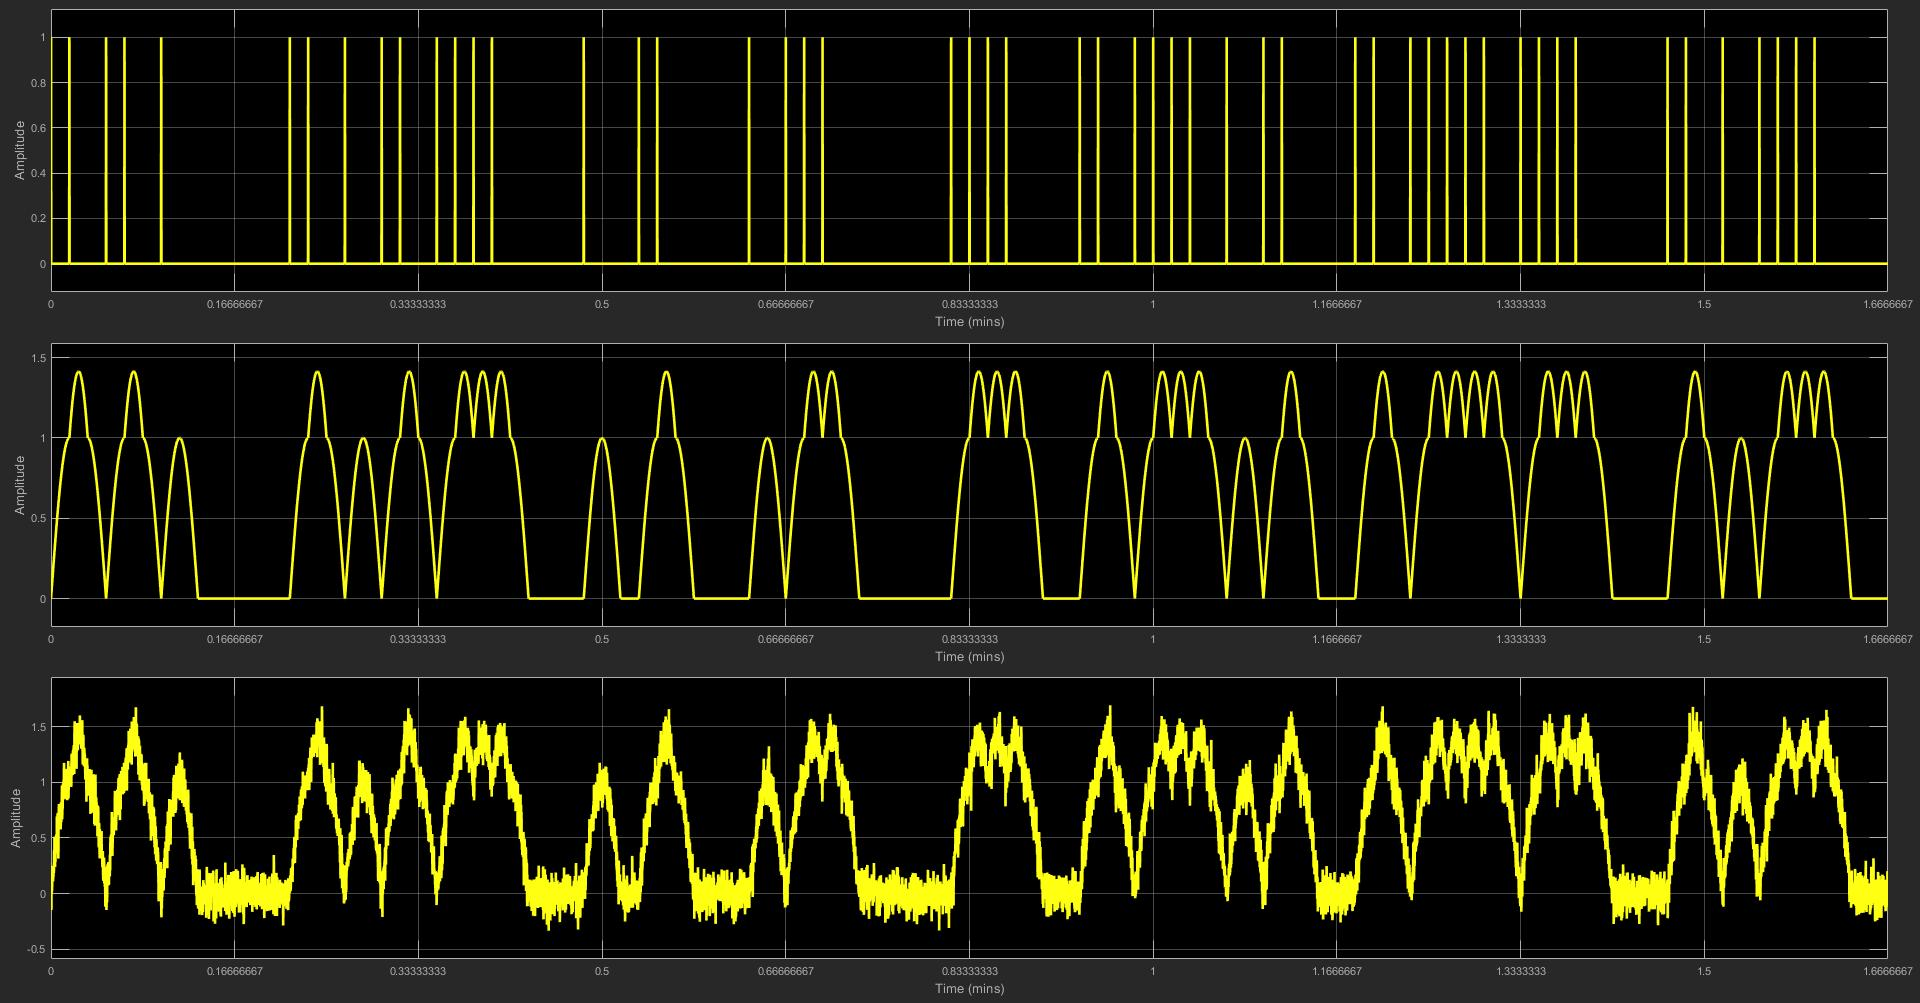
\includegraphics[width = \linewidth]{OO_Sin.jpg}
  \caption{On-Off encoding with a Full Width Rectangle Shaped Pulse}
  \label{fig:OO-Sin}
\end{figure}
\begin{figure}[H]
  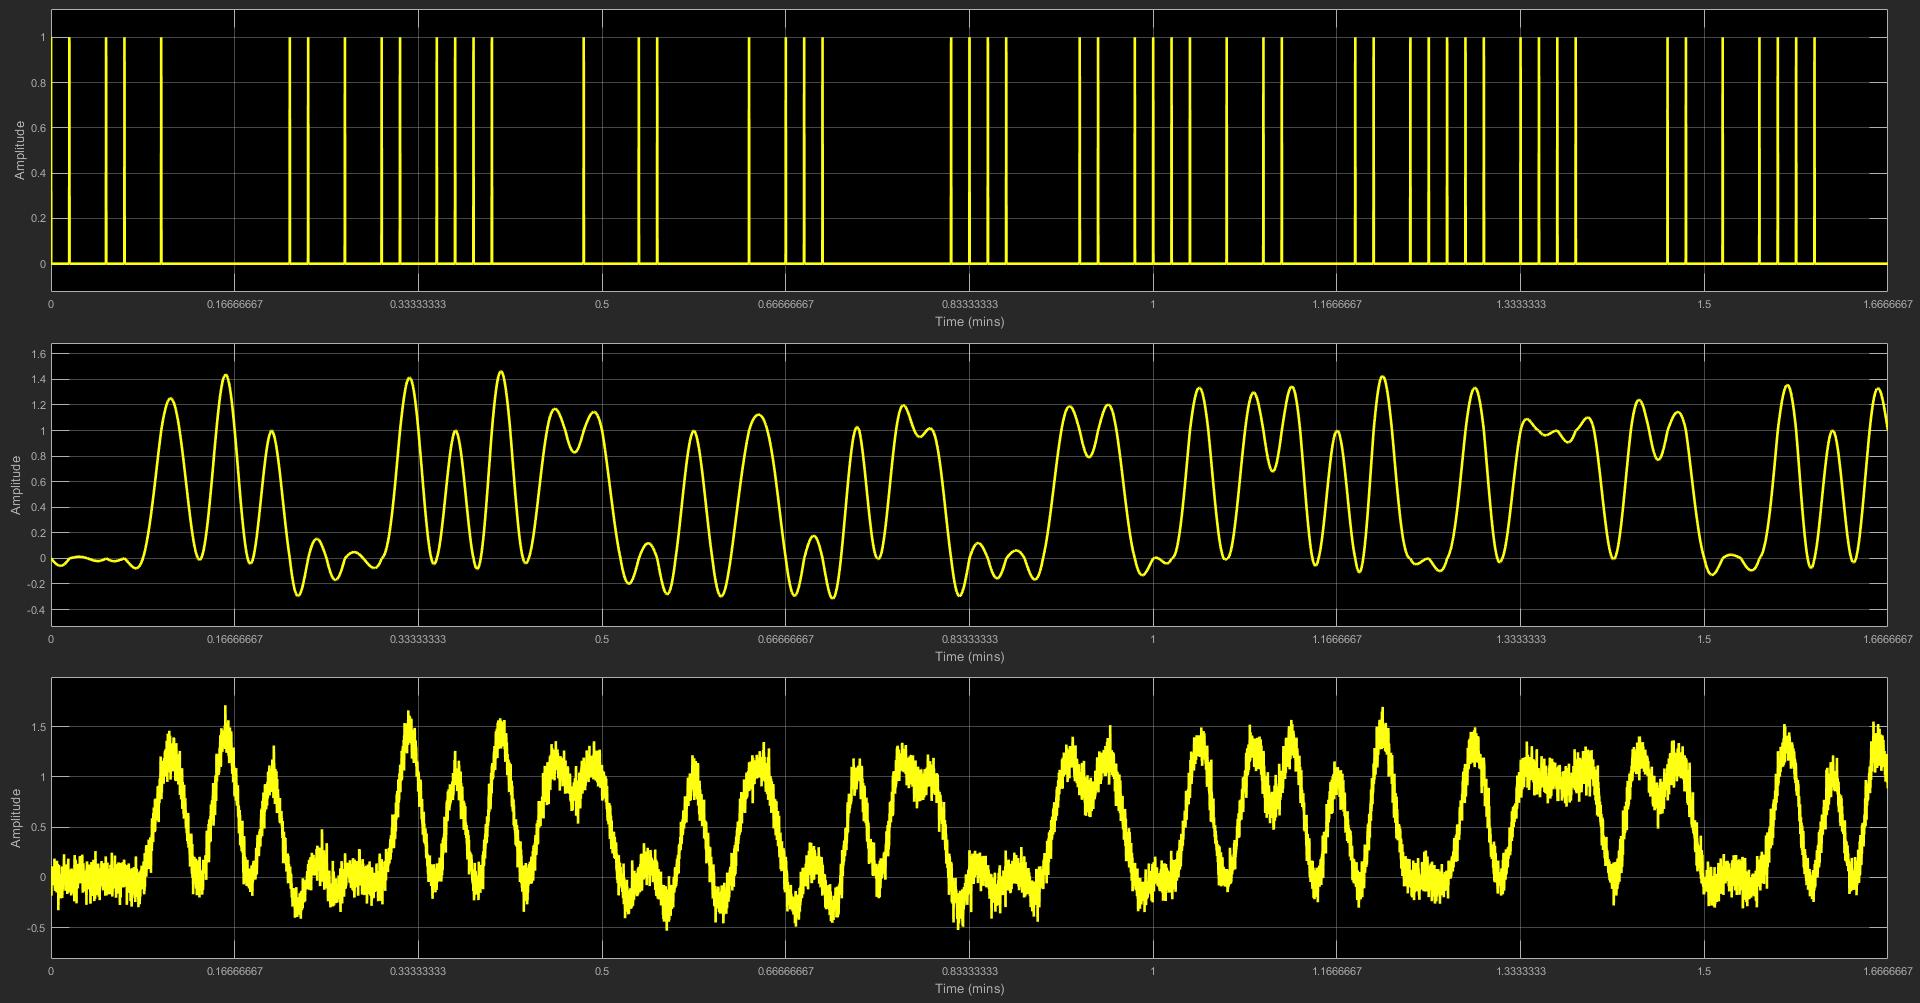
\includegraphics[width = \linewidth]{OO_Sinc.jpg}
  \caption{On-Off encoding with a Sinc Shaped Pulse}
  \label{fig:OO-Sinc}
\end{figure}
\begin{figure}[H]
  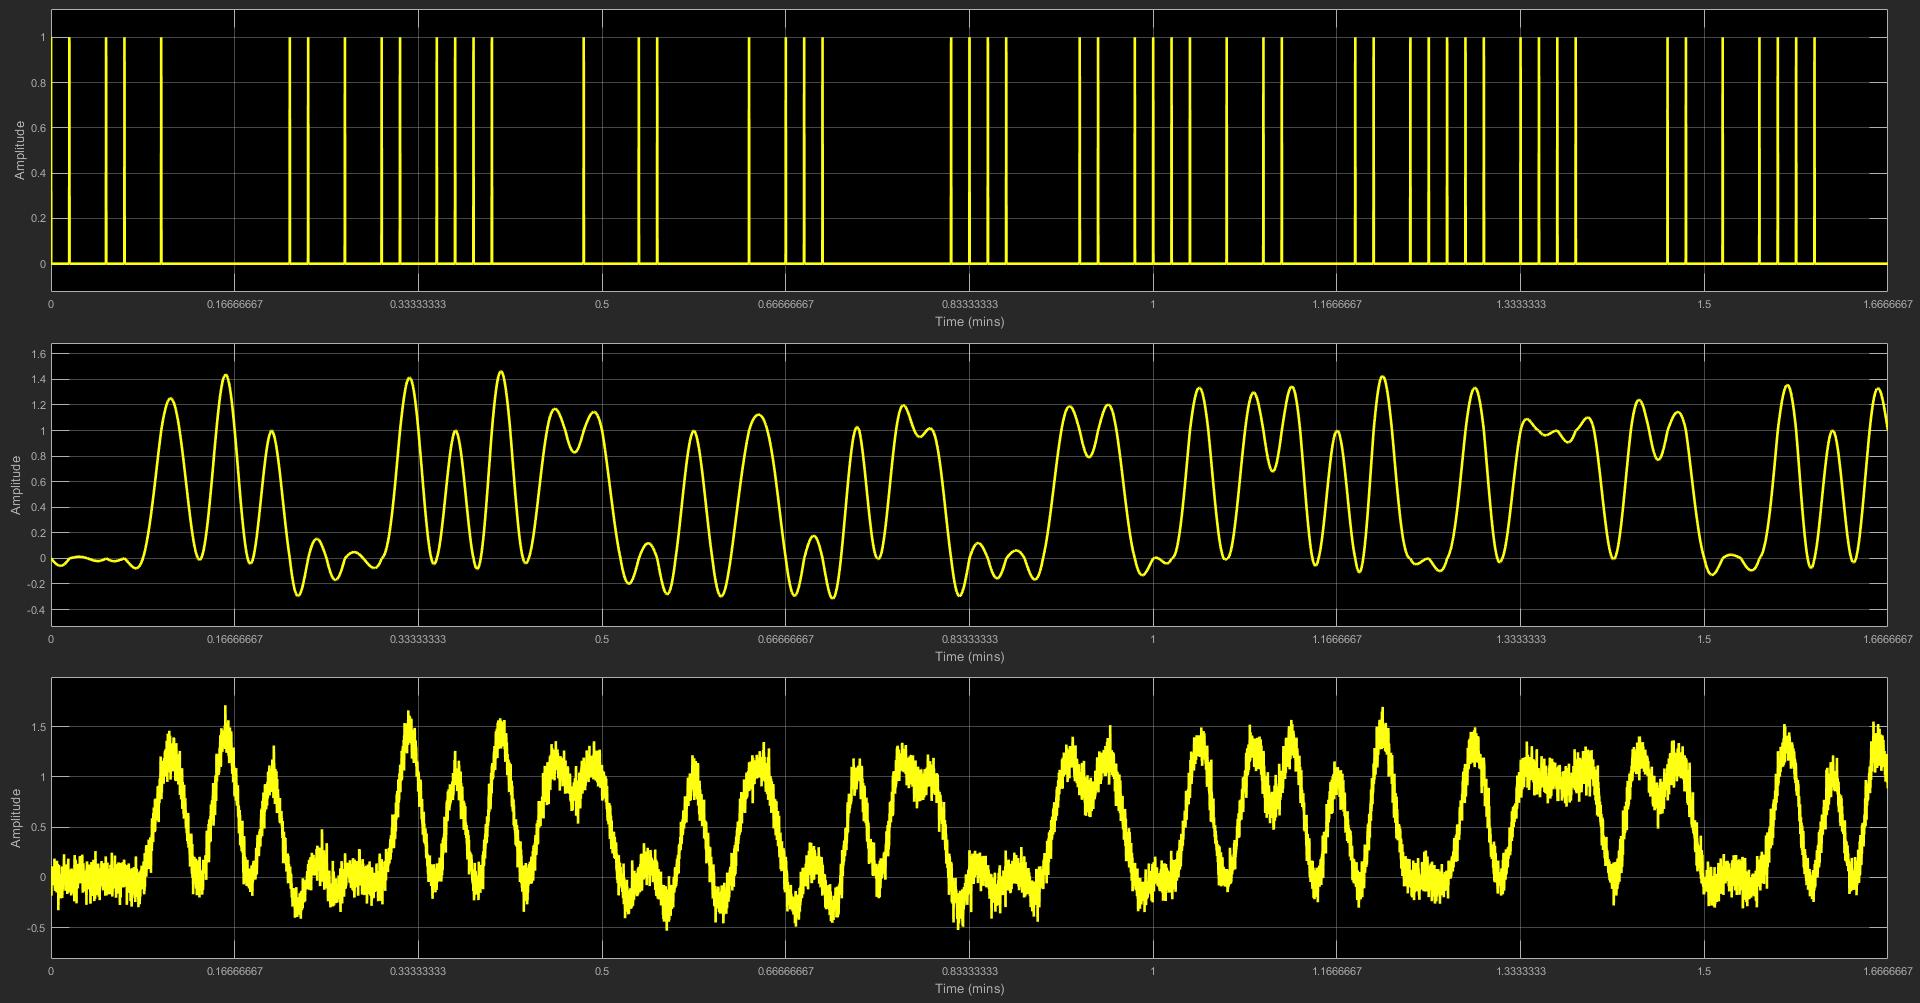
\includegraphics[width = \linewidth]{OO_Squared.jpg}
  \caption{On-Off encoding with a Sinc Squared Shaped Pulse}
  \label{fig:OO-Squared}
\end{figure}
\begin{figure}[H]
  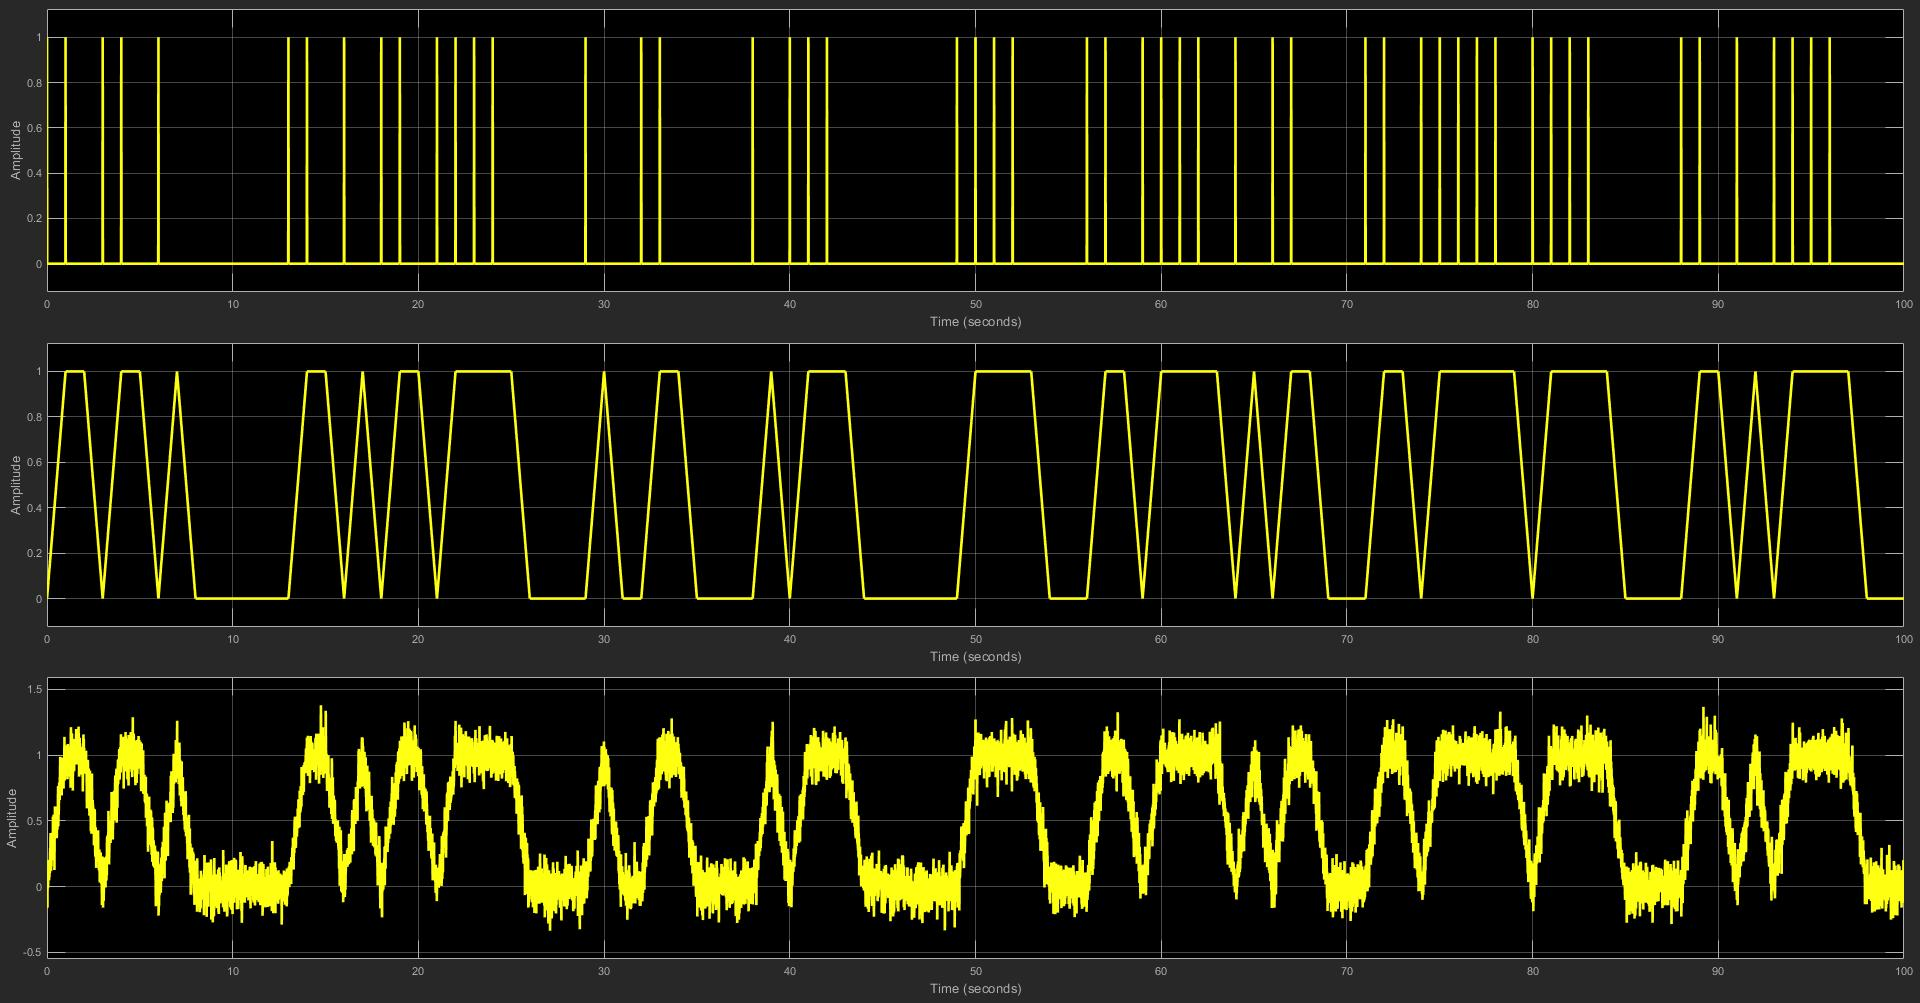
\includegraphics[width = \linewidth]{OO_Tri_F.jpg}
  \caption{On-Off encoding with a Full Width Triangle Shaped Pulse}
  \label{fig:OO-Tri-F}
\end{figure}
\begin{figure}[H]
  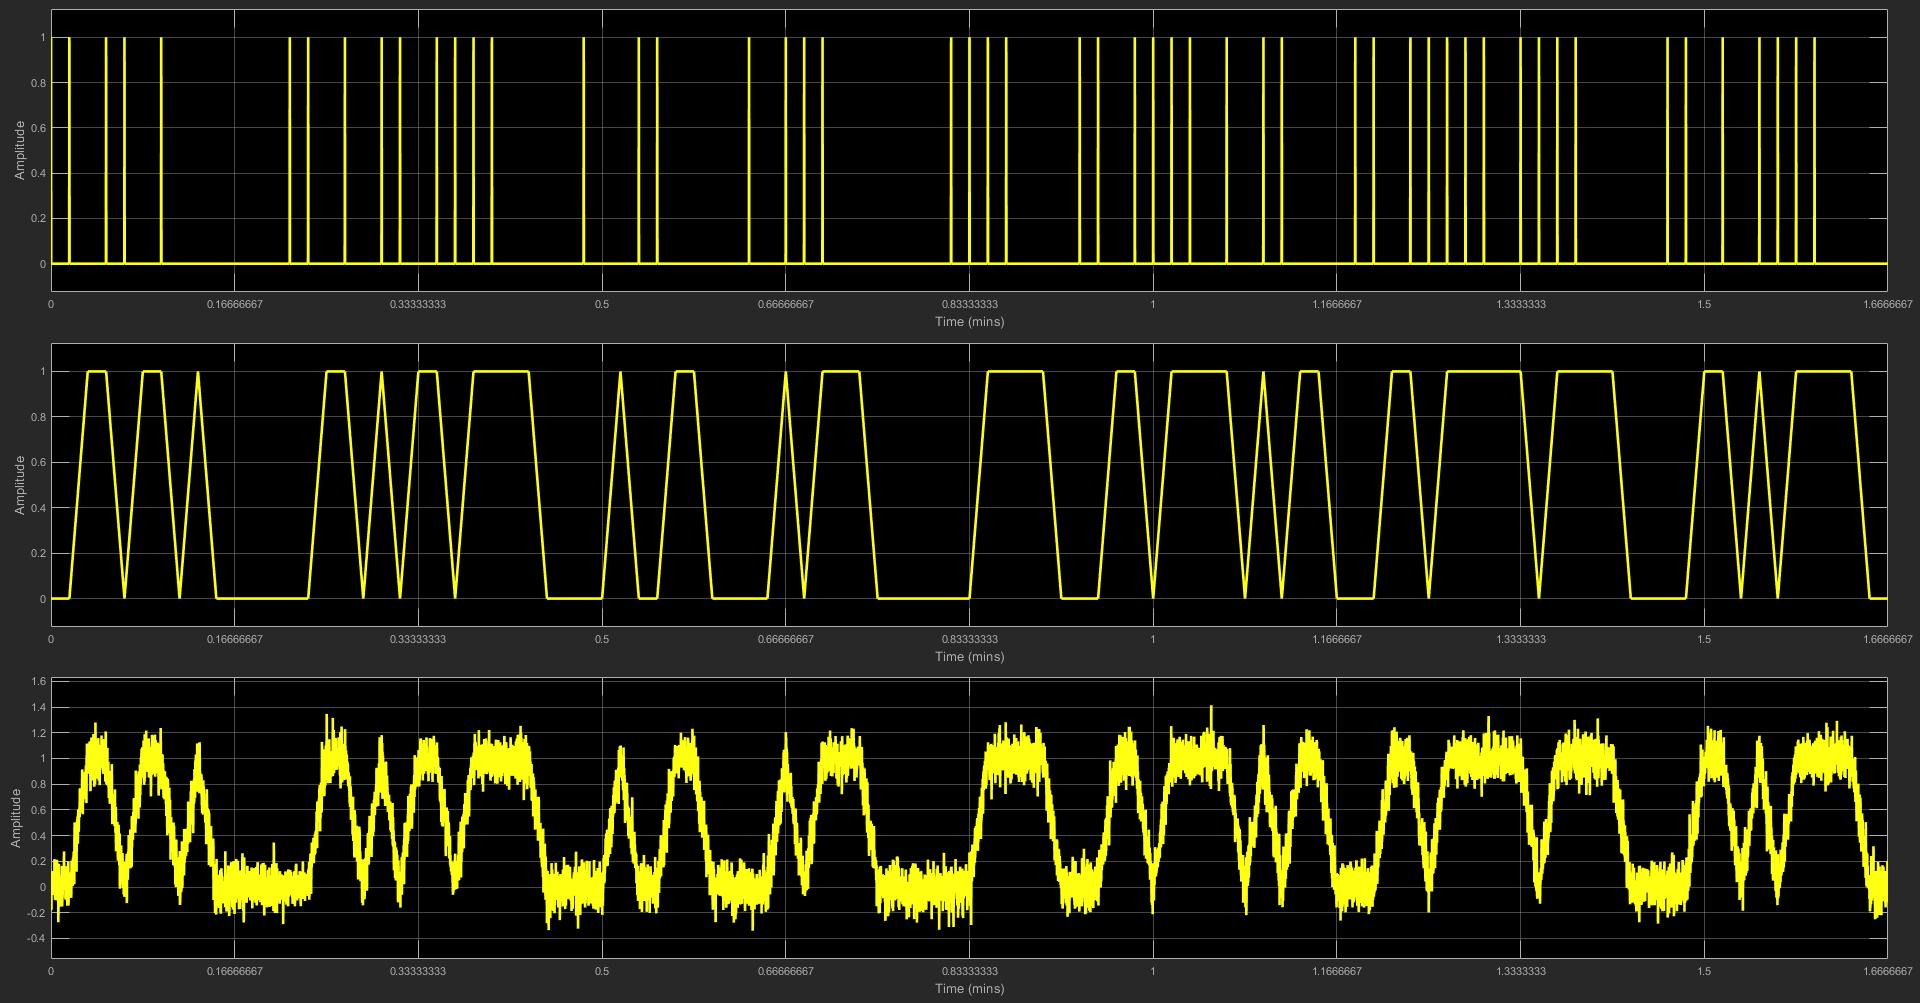
\includegraphics[width = \linewidth]{OO_Tri_H.jpg}
  \caption{On-Off encoding with a Half Width Triangle Shaped Pulse}
  \label{fig:OO-Tri-H}
\end{figure}
Something that should be noted is that the apparent difference between full width and half with shaped pulses for both Rectangle and Triangle shaped pulses have an identical waveform. The difference is the half width is a delayed signal.
\subsubsection{Eye Diagrams}
\begin{figure}[H]
  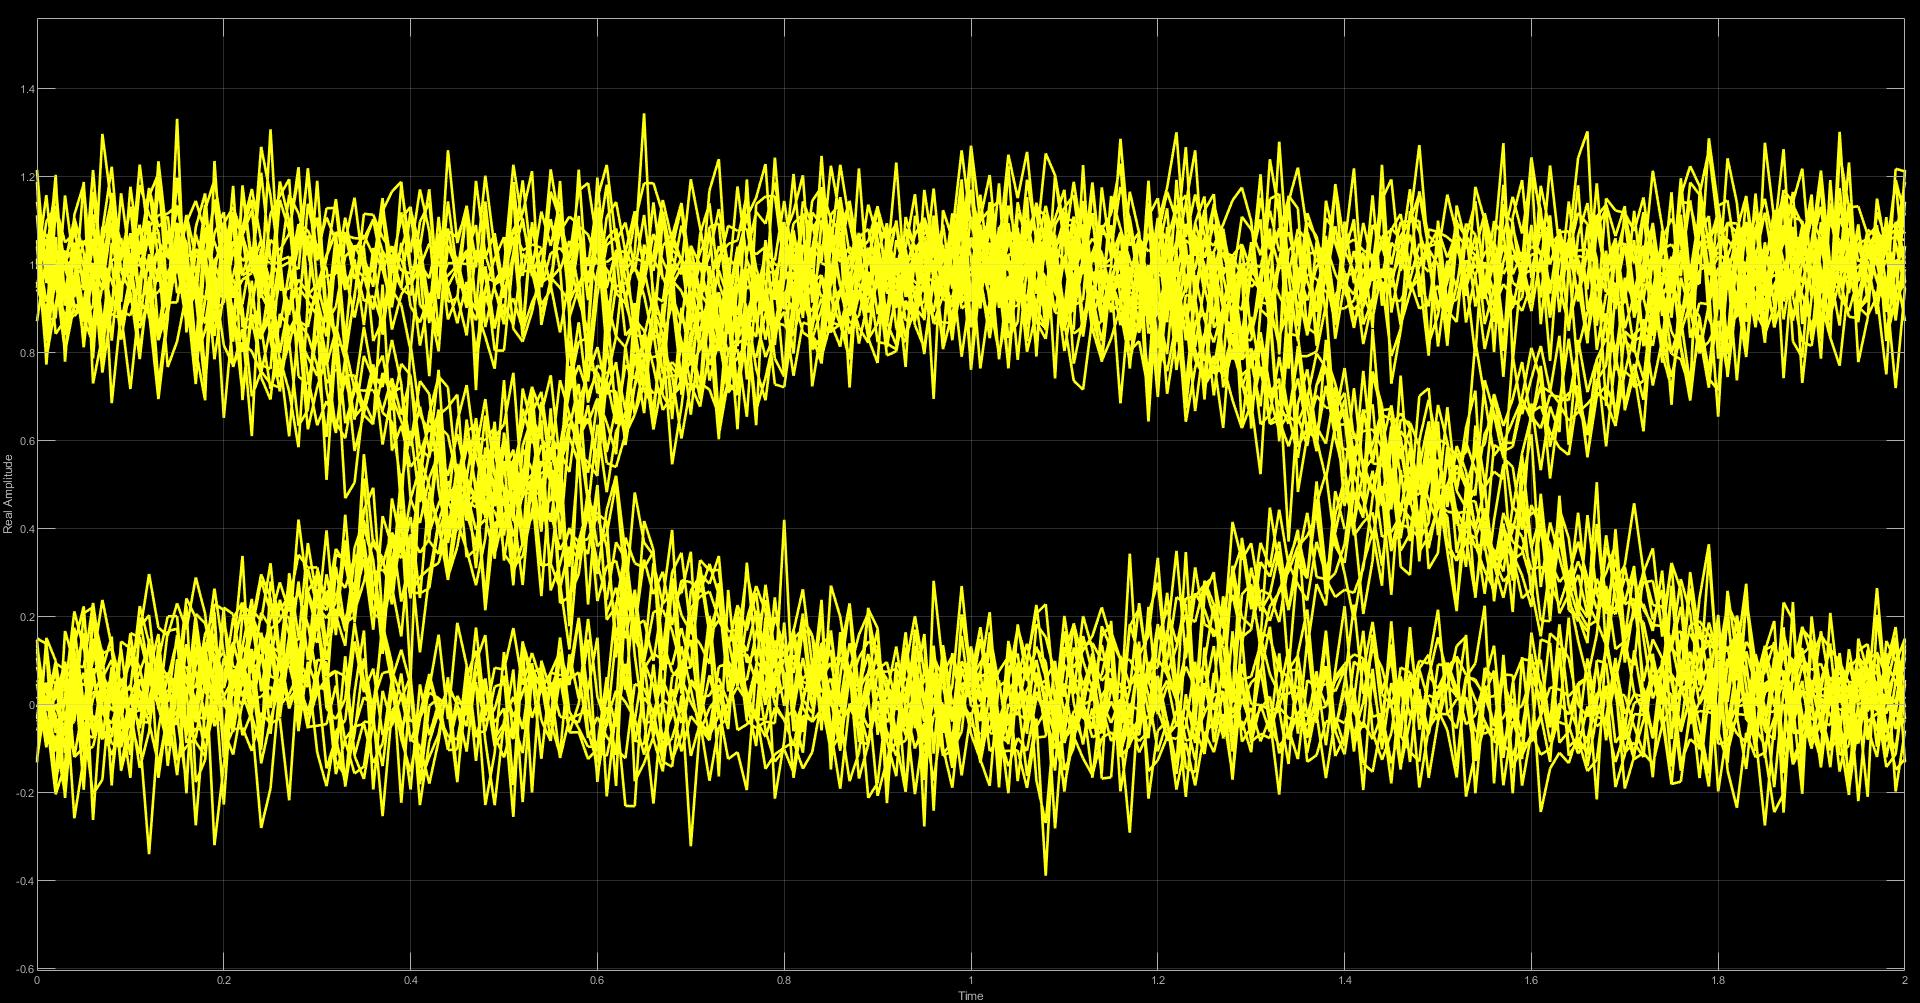
\includegraphics[width = \linewidth]{OO_Rasied_Eye.jpg}
  \caption{Eye Diagram for On-Off encoding with a Raised Cosine Shaped Pulse}
  \label{fig:OO-Raised-Eye}
\end{figure}
\begin{figure}[H]
  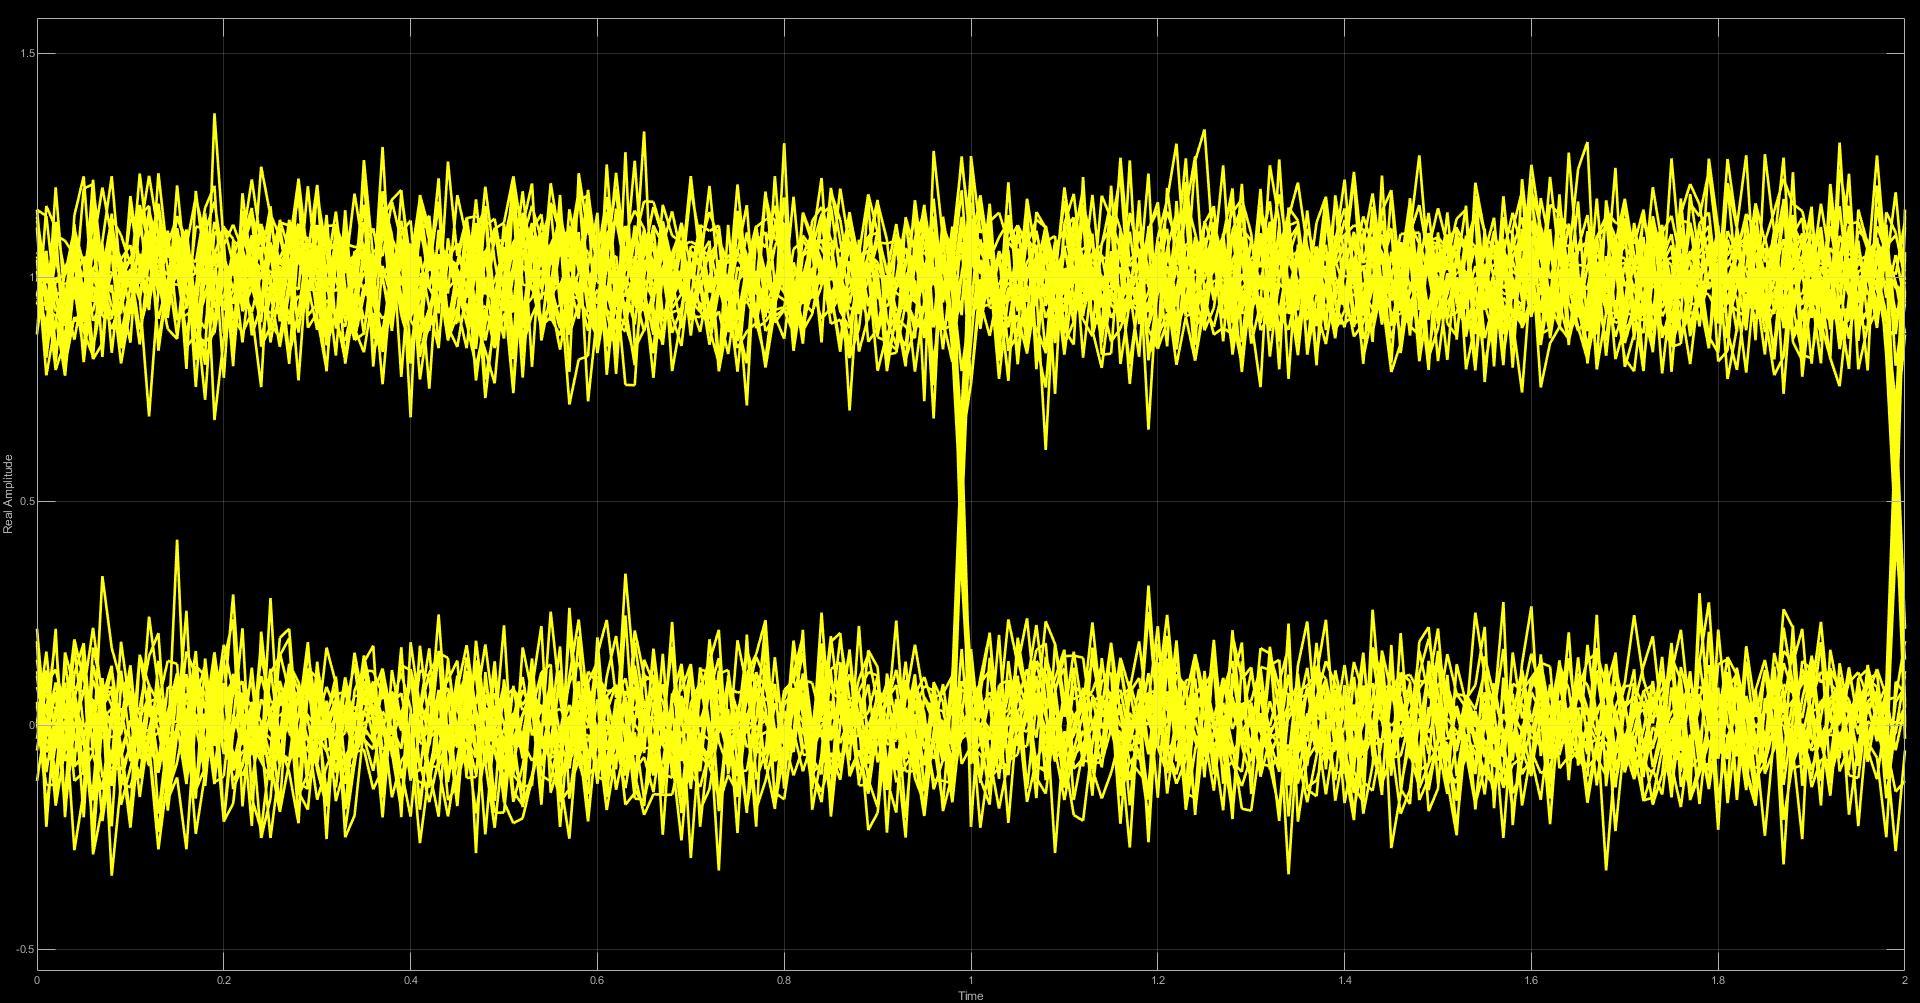
\includegraphics[width = \linewidth]{OO_Rect_F_Eye.jpg}
  \caption{Eye Diagram for On-Off encoding with a Full Width Rectangle Shaped Pulse}
  \label{fig:OO-Rect-F-Eye}
\end{figure}
\begin{figure}[H]
  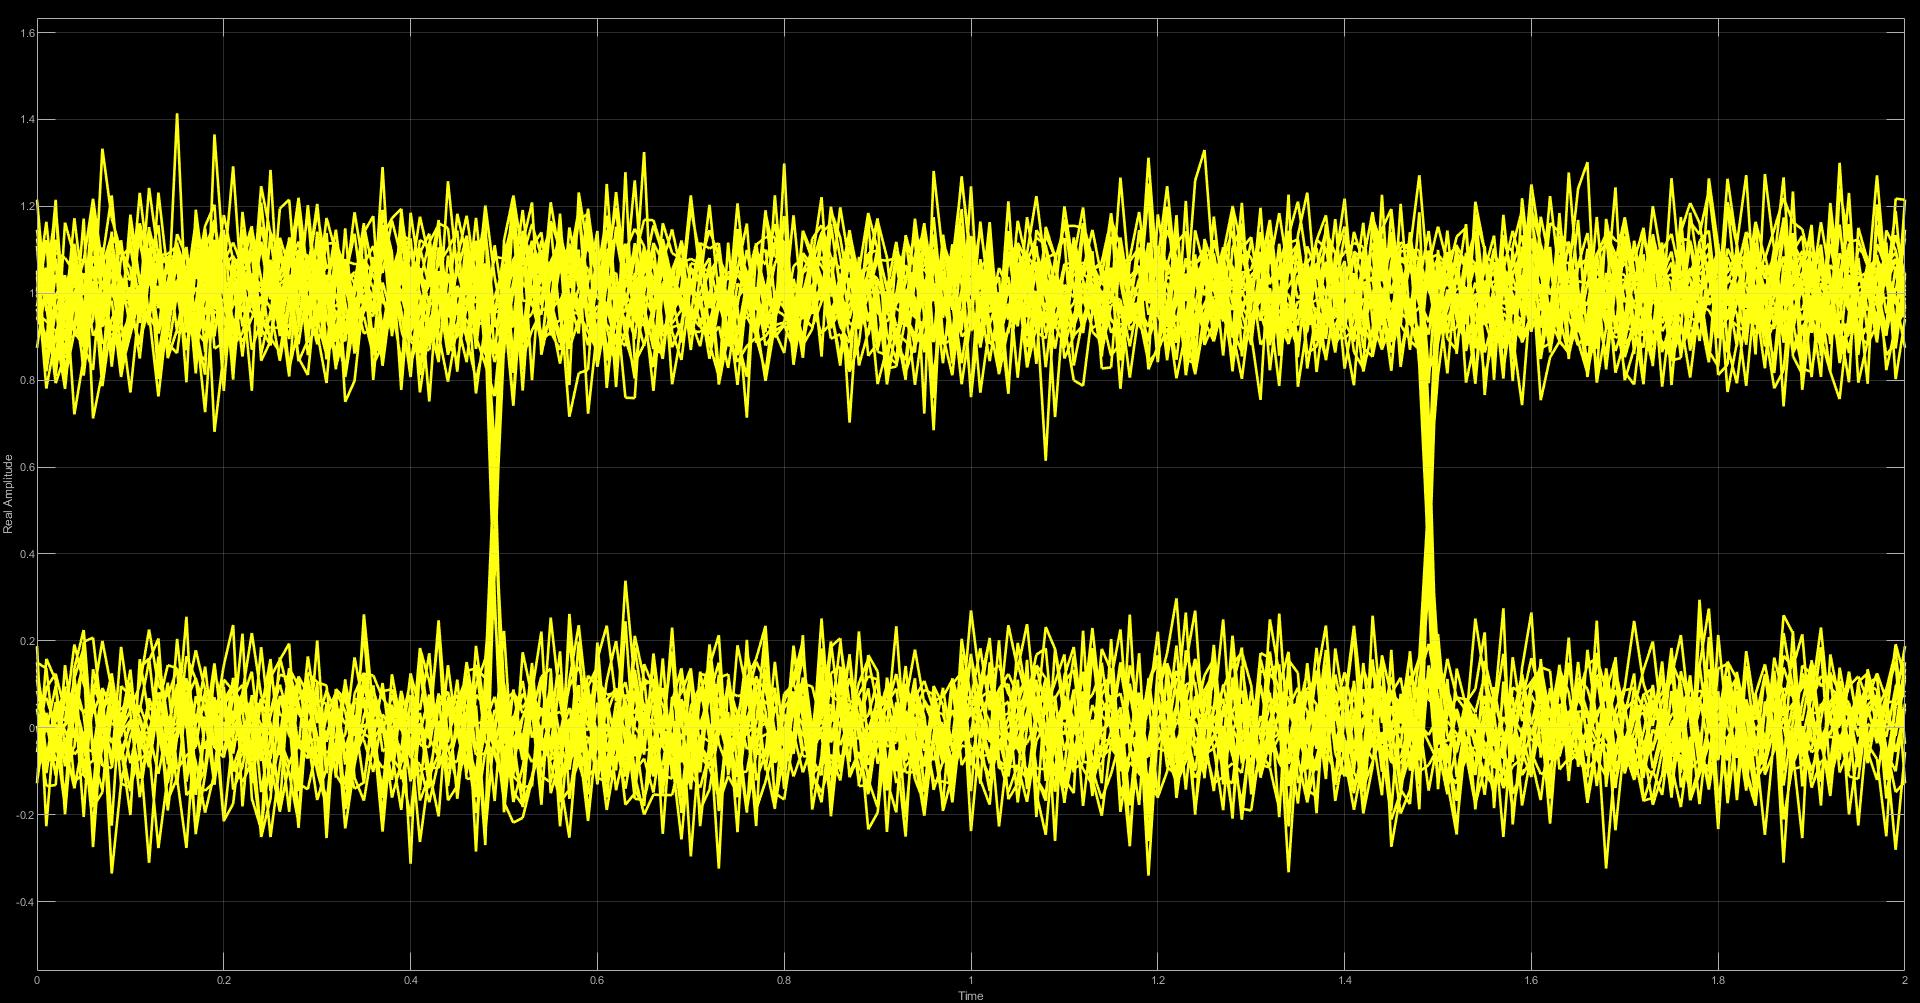
\includegraphics[width = \linewidth]{OO_Rect_H_Eye.jpg}
  \caption{Eye Diagram for On-Off encoding with a Half Width Rectangle Shaped Pulse}
  \label{fig:OO-Rect-H-Eye}
\end{figure}
\begin{figure}[H]
  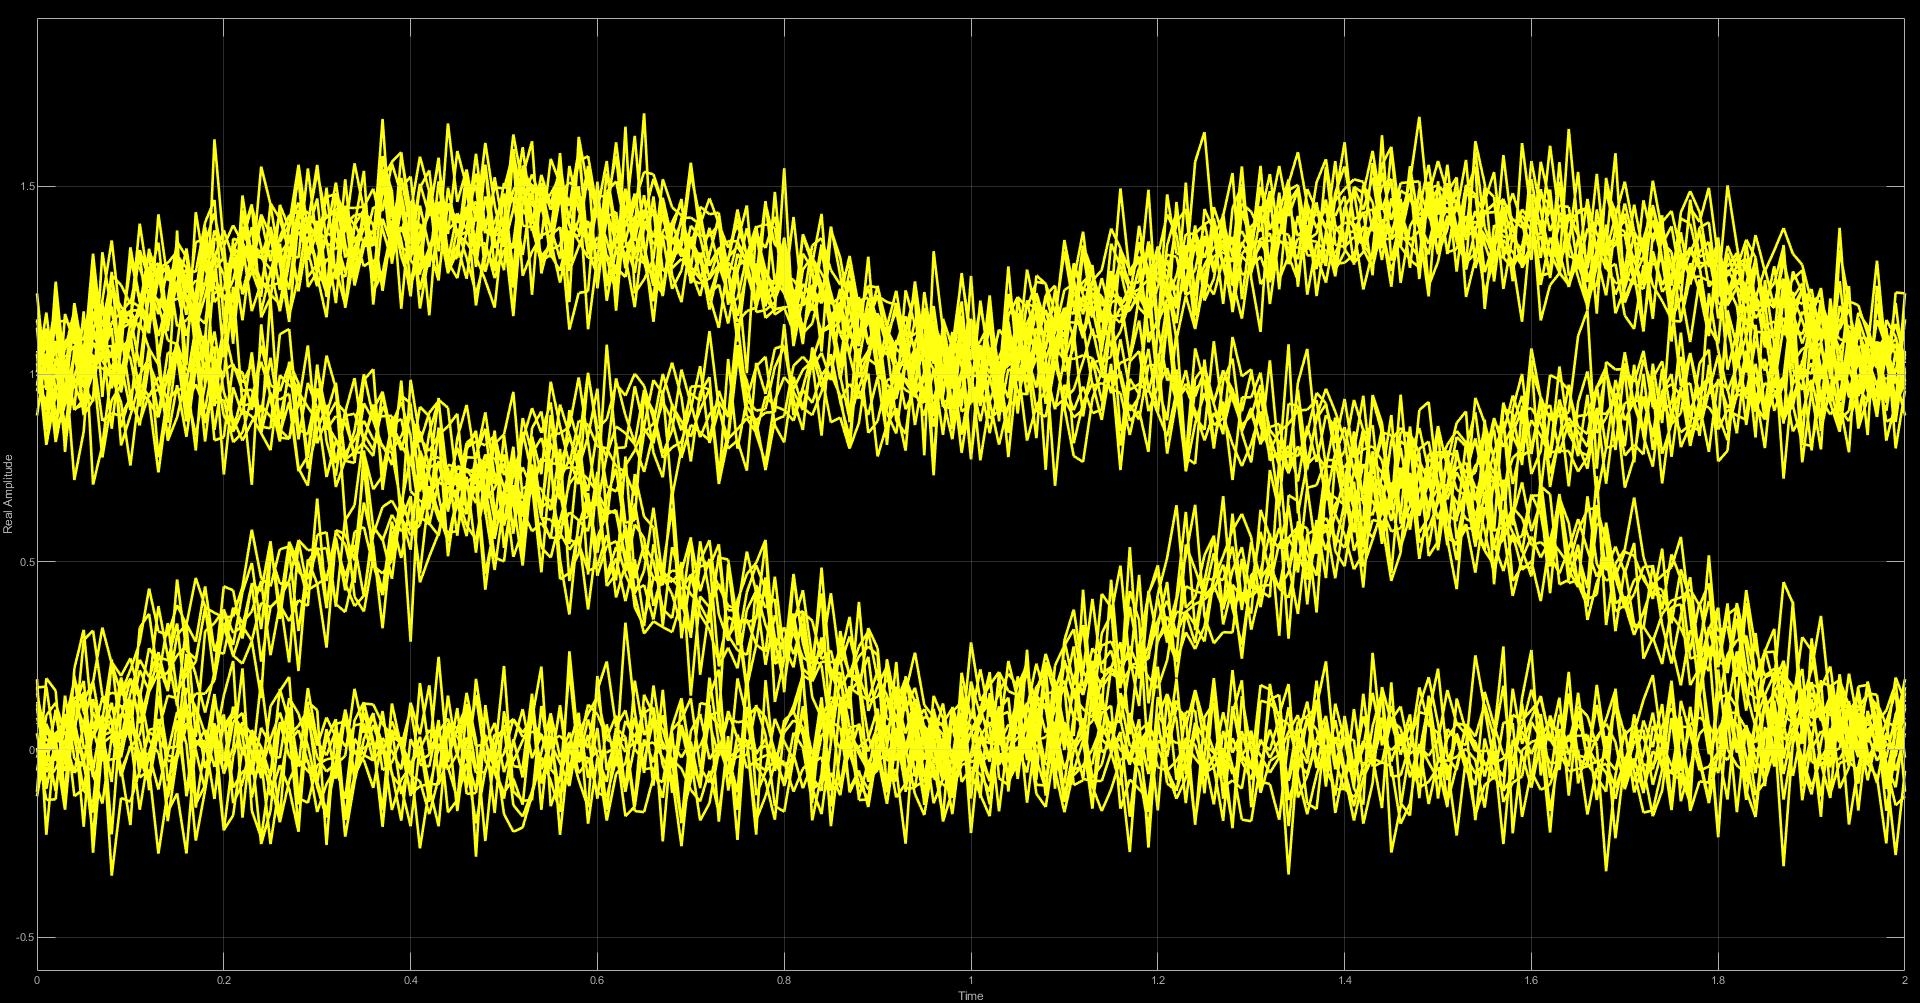
\includegraphics[width = \linewidth]{OO_Sin_Eye.jpg}
  \caption{Eye Diagram for On-Off encoding with a Full Width Rectangle Shaped Pulse}
  \label{fig:OO-Sin-Eye}
\end{figure}
\begin{figure}[H]
  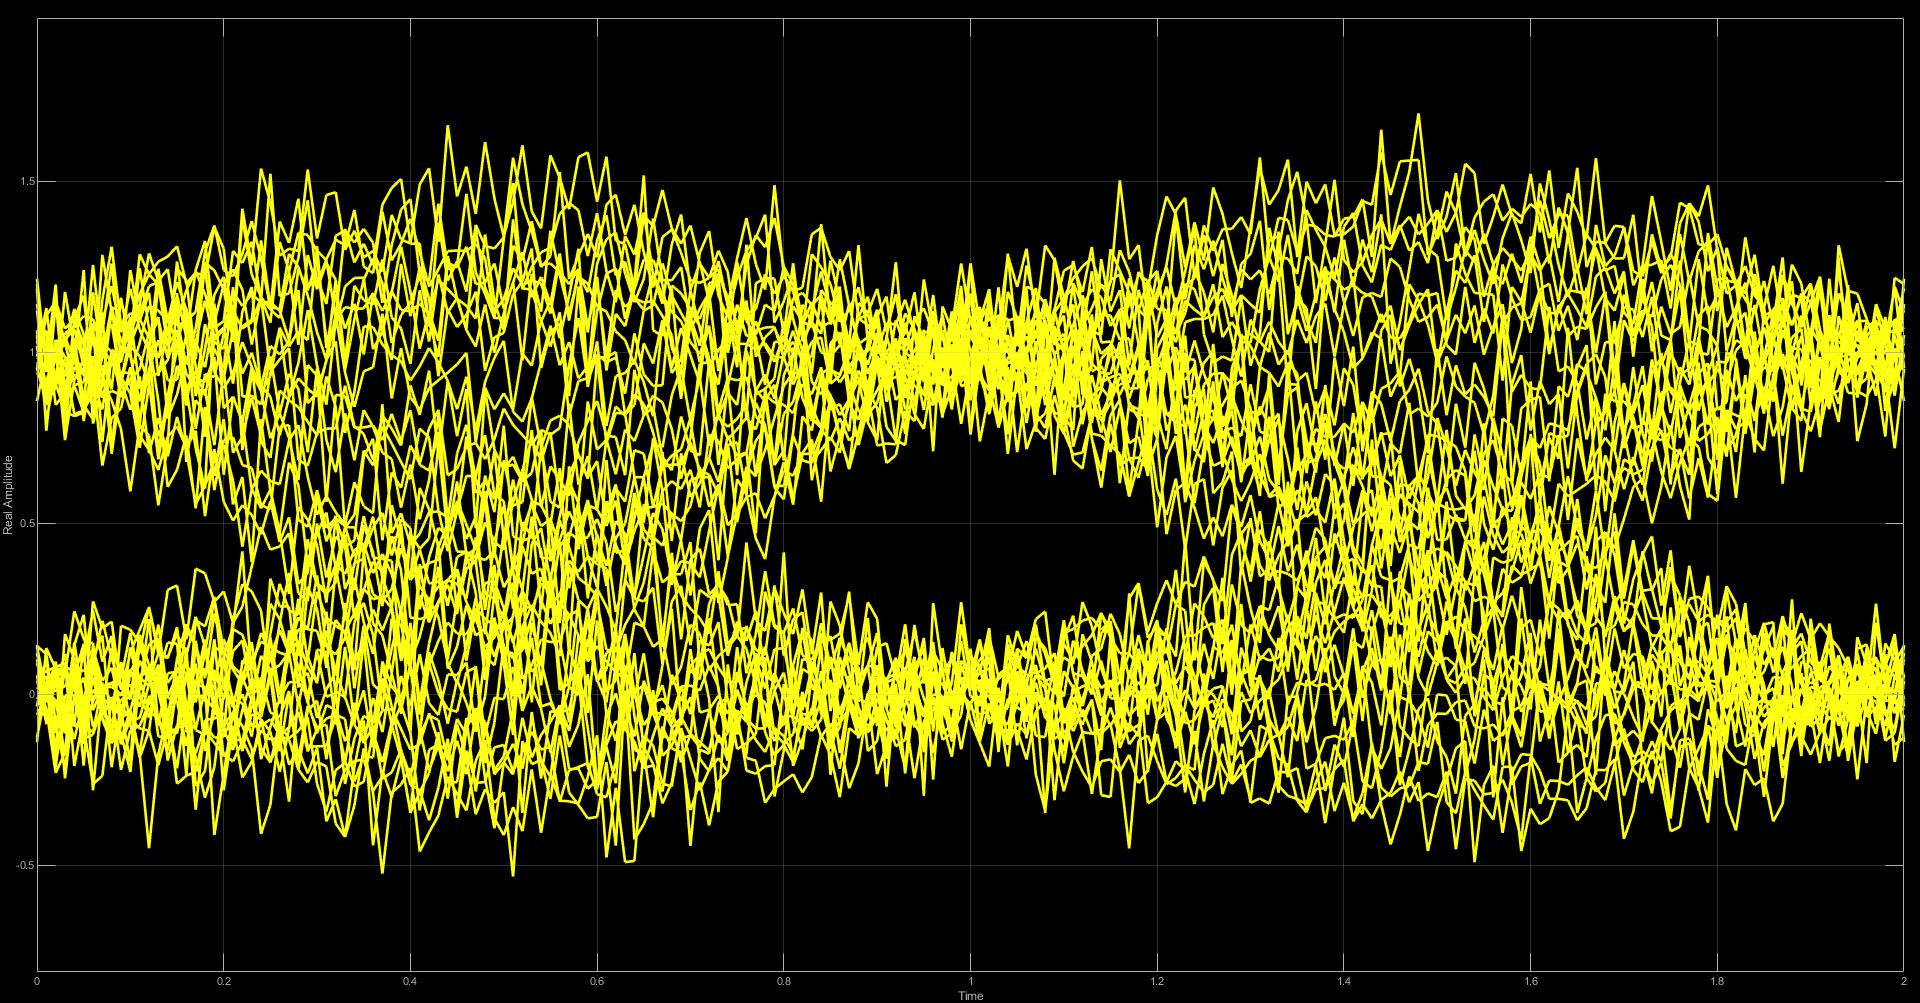
\includegraphics[width = \linewidth]{OO_Sinc_Eye.jpg}
  \caption{Eye Diagram for On-Off encoding with a Sinc Shaped Pulse}
  \label{fig:OO-Sinc-Eye}
\end{figure}
\begin{figure}[H]
  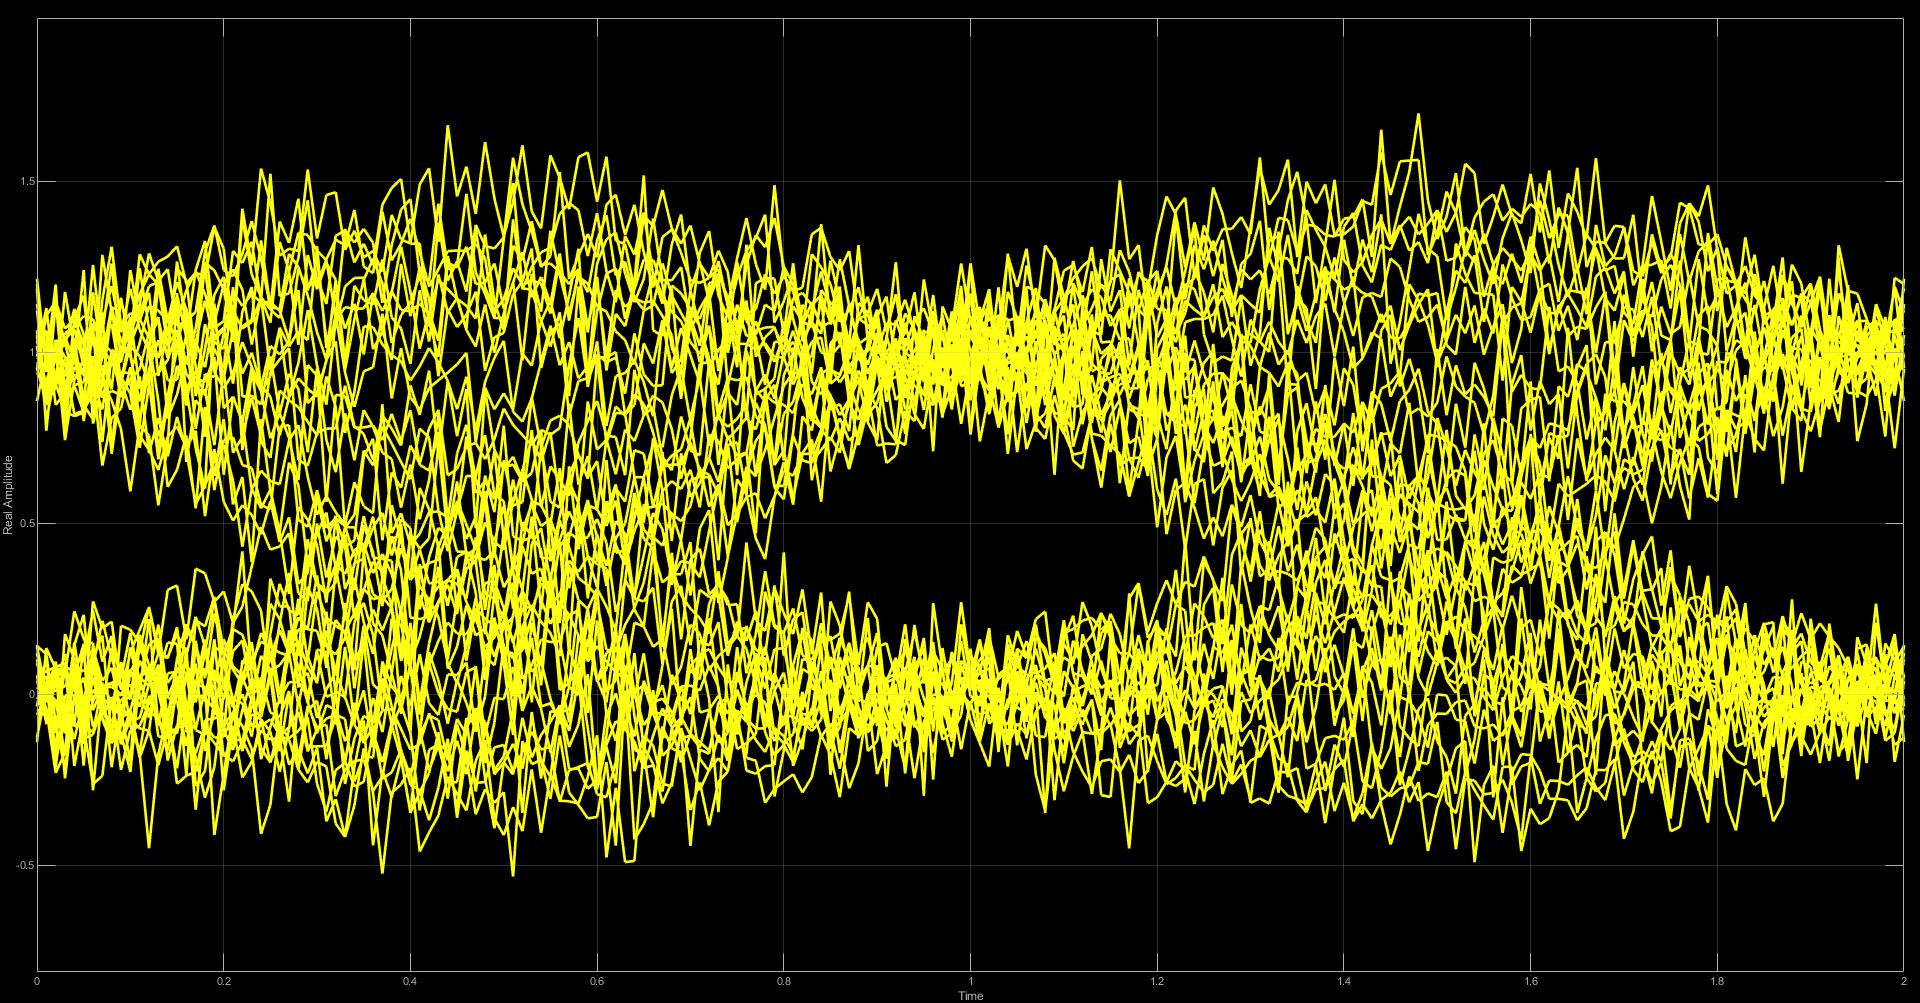
\includegraphics[width = \linewidth]{OO_Squared_Eye.jpg}
  \caption{Eye Diagram for On-Off encoding with a Sinc Squared Shaped Pulse}
  \label{fig:OO-Squared-Eye}
\end{figure}
\begin{figure}[H]
  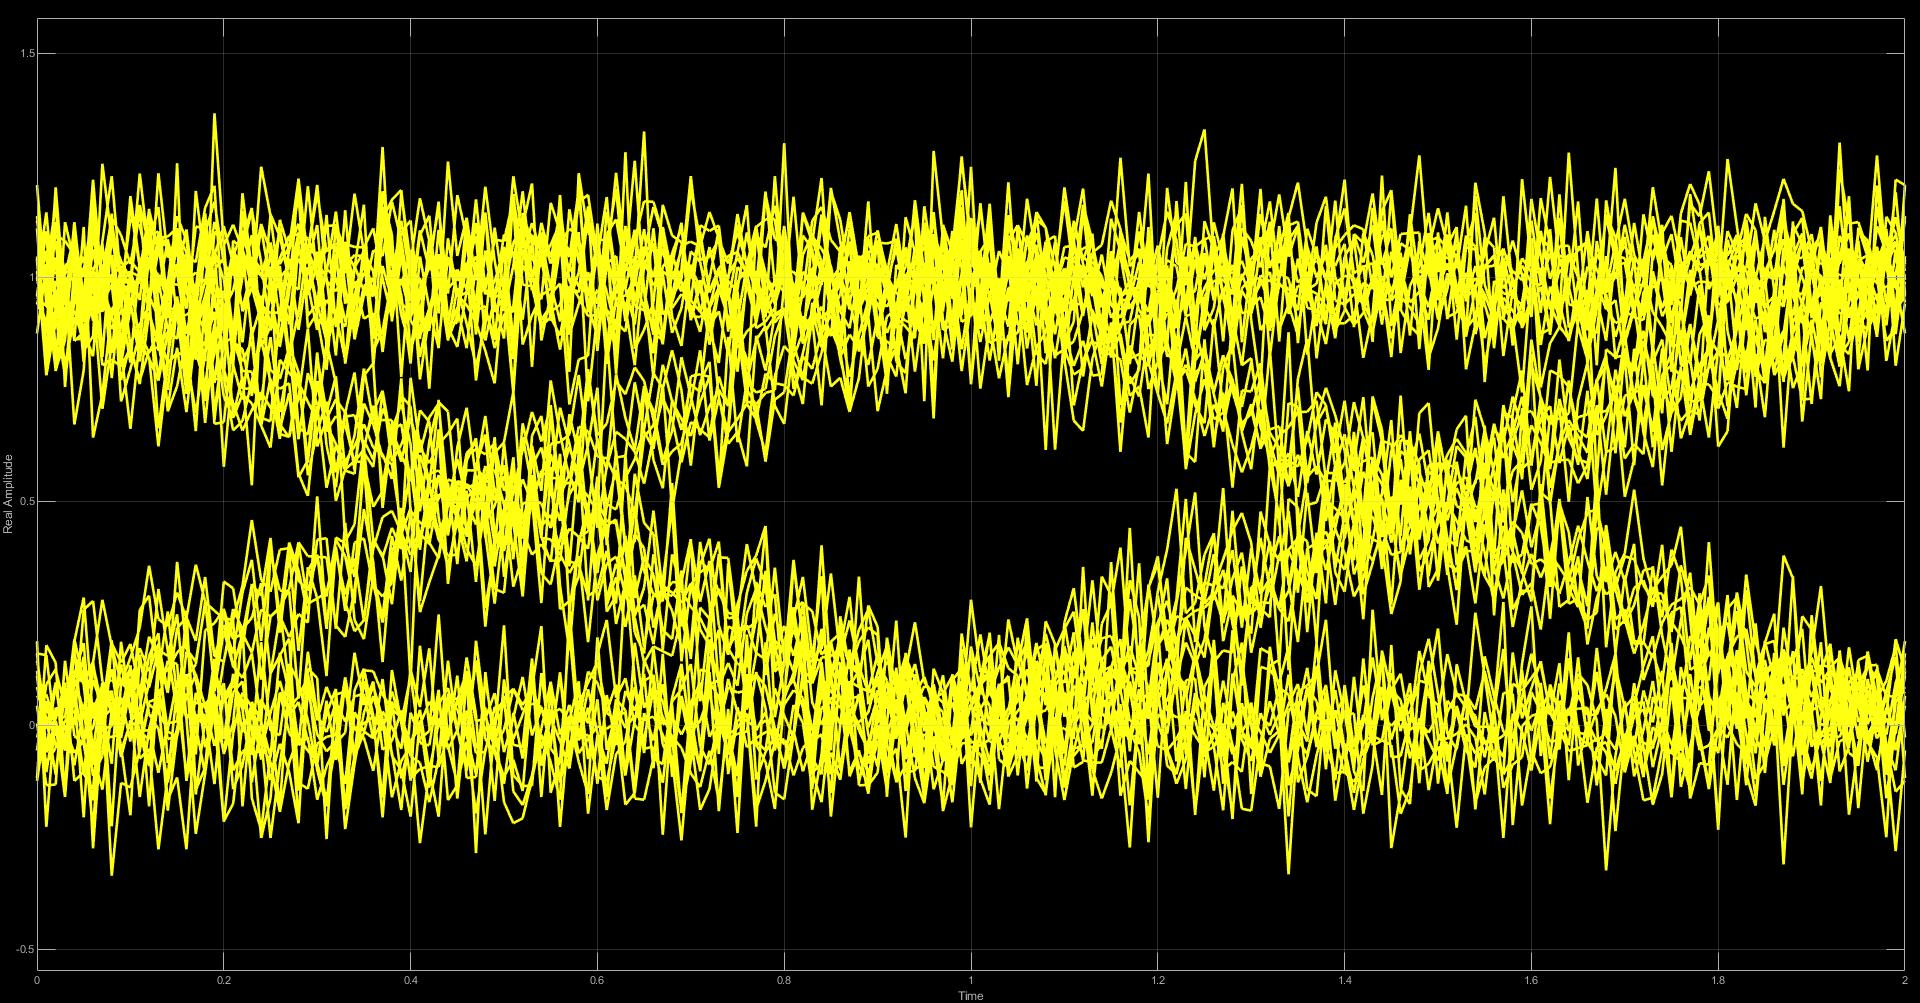
\includegraphics[width = \linewidth]{OO_Tri_F_Eye.jpg}
  \caption{Eye Diagram for On-Off encoding with a Full Width Triangle Shaped Pulse}
  \label{fig:OO-Tri-F-Eye}
\end{figure}
\begin{figure}[H]
  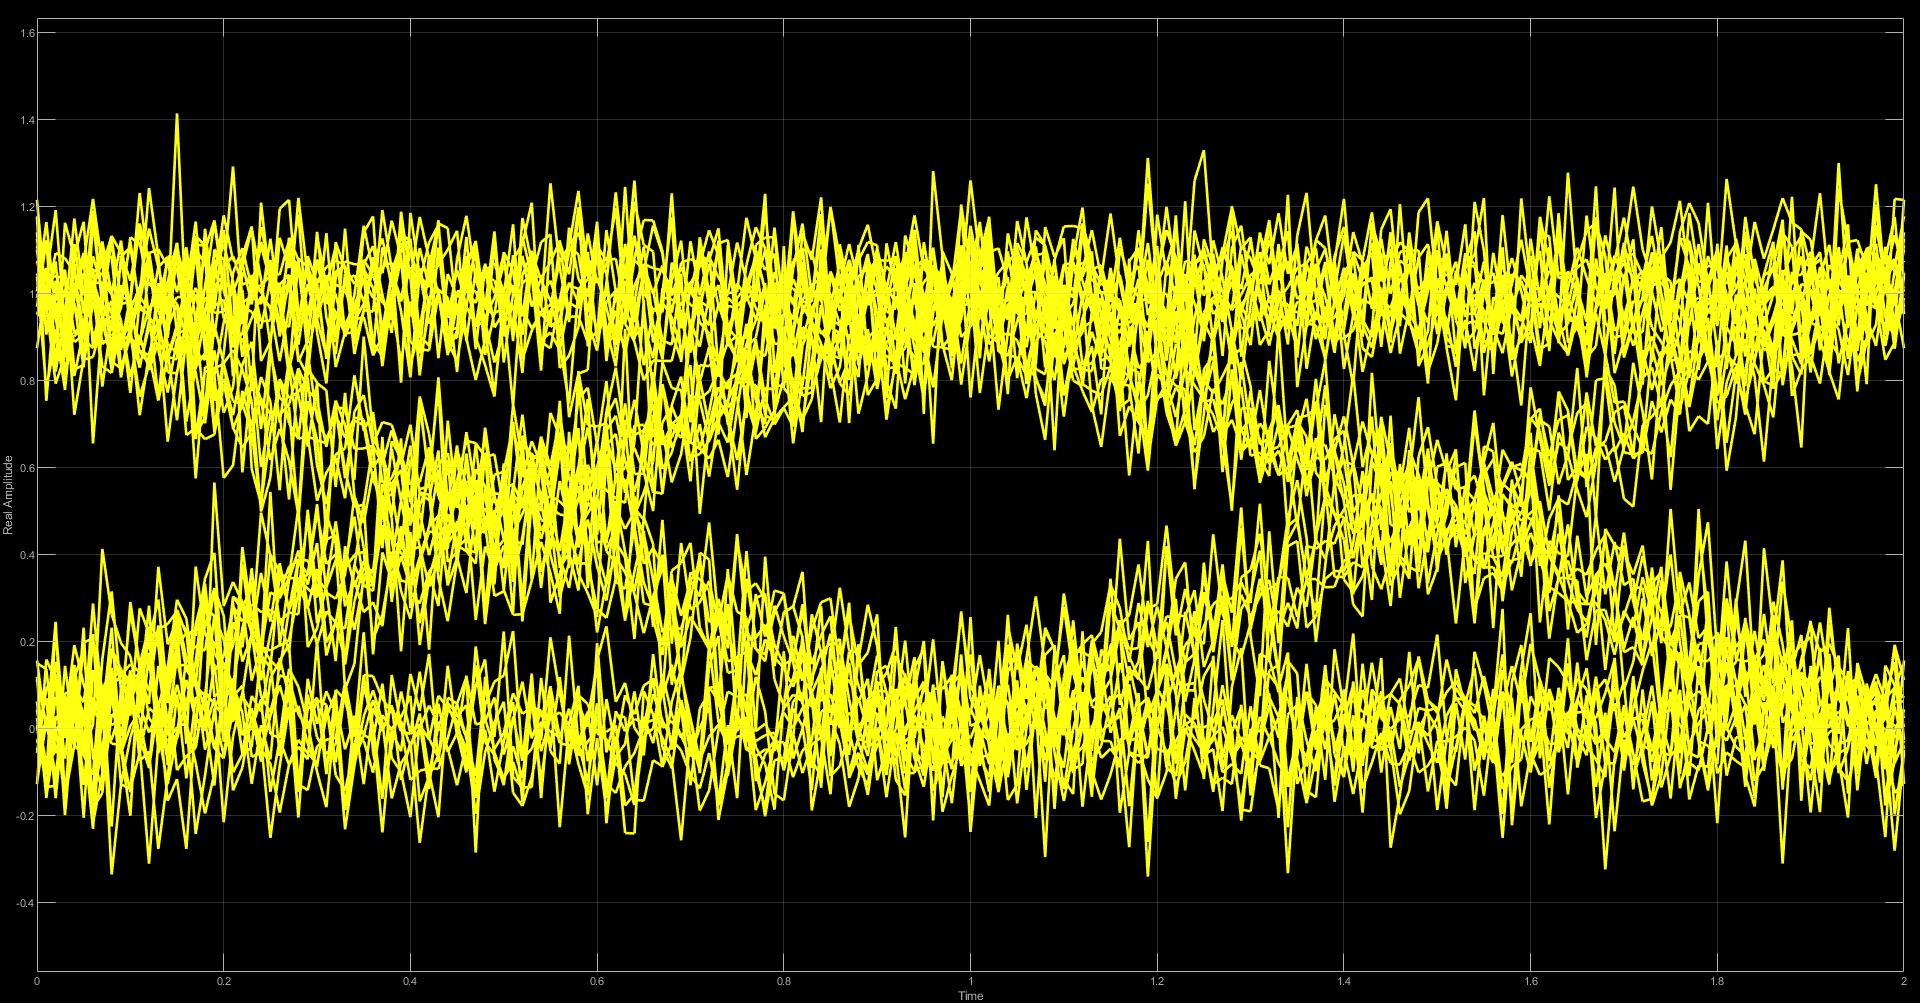
\includegraphics[width = \linewidth]{OO_Tri_H_Eye.jpg}
  \caption{Eye Diagram for On-Off encoding with a Half Width Triangle Shaped Pulse}
  \label{fig:OO-Tri-H-Eye}
\end{figure}
When looking at the eye diagrams, it can be seen in the full and half width rectangle pulses that in the half width shaped pulse the decision instant is offset by half the period of the signal.
\subsubsection{Spectrum}
\begin{figure}[H]
  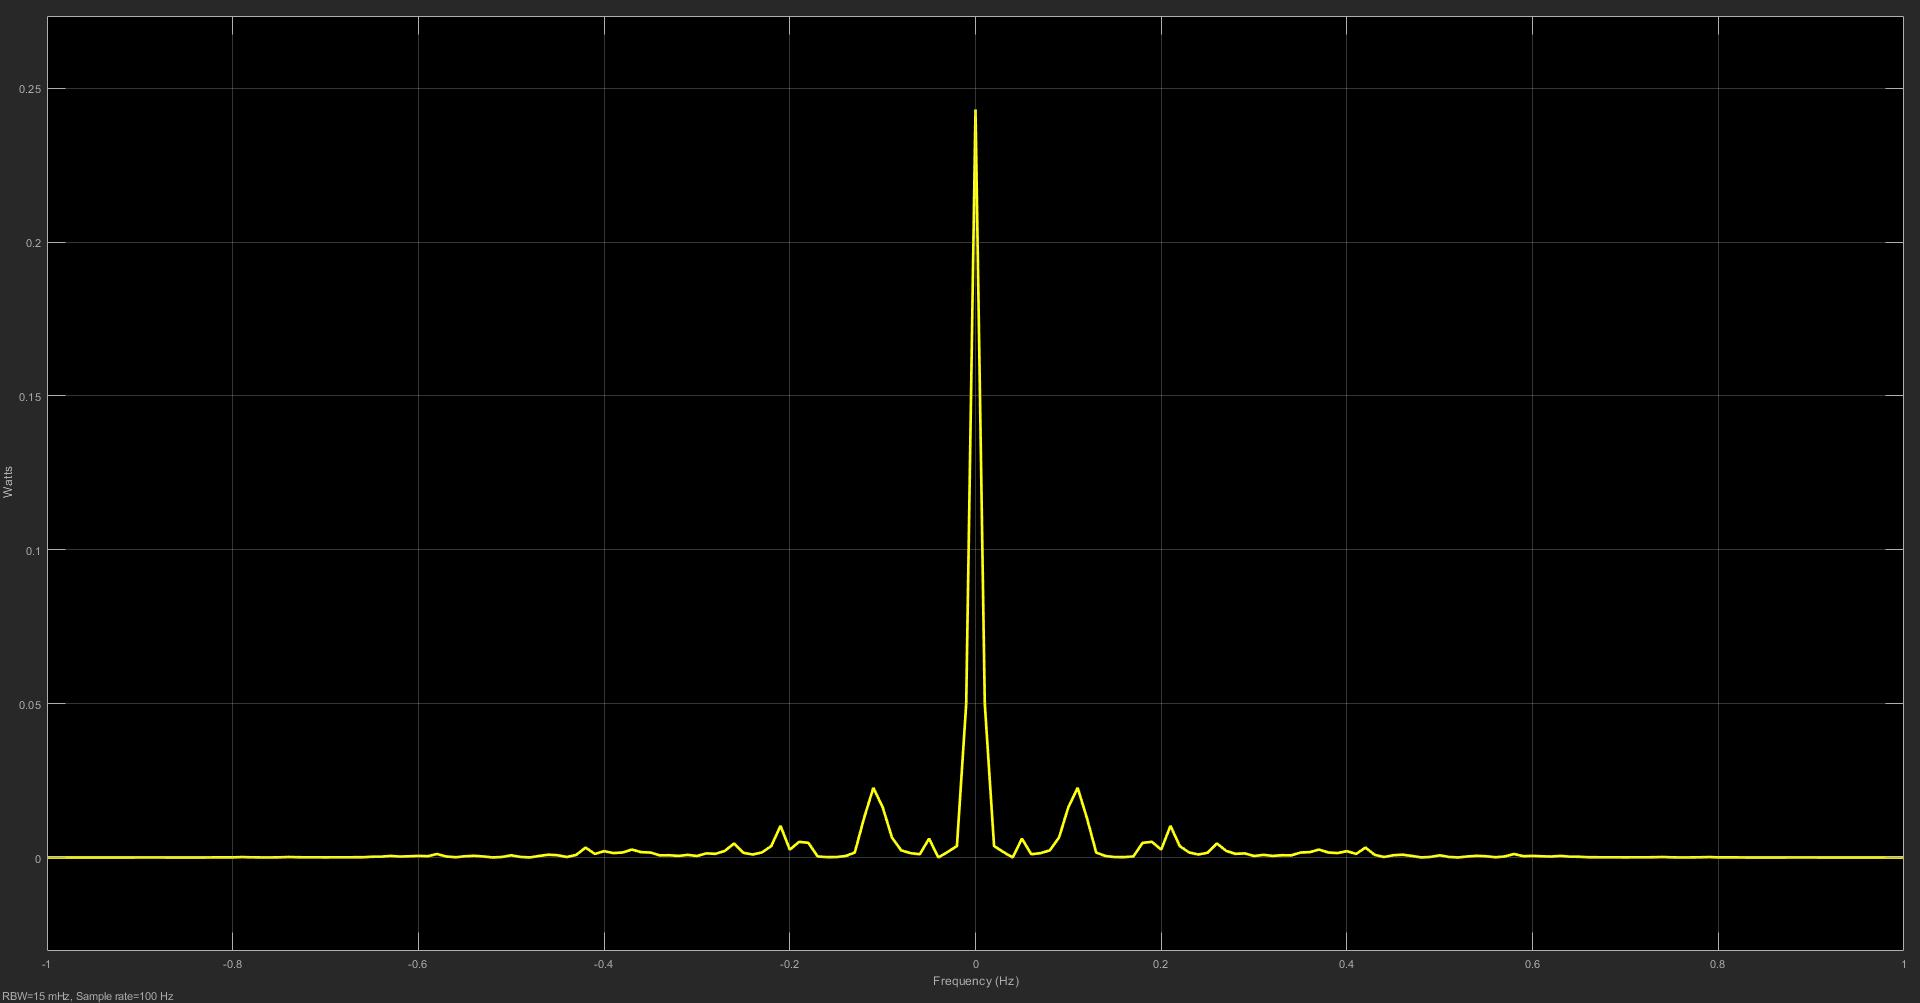
\includegraphics[width = \linewidth]{OO_Rasied_Spectrum.jpg}
  \caption{Spectrum for On-Off encoding with a Raised Cosine Shaped Pulse}
  \label{fig:OO-Raised-Spectrum}
\end{figure}
\begin{figure}[H]
  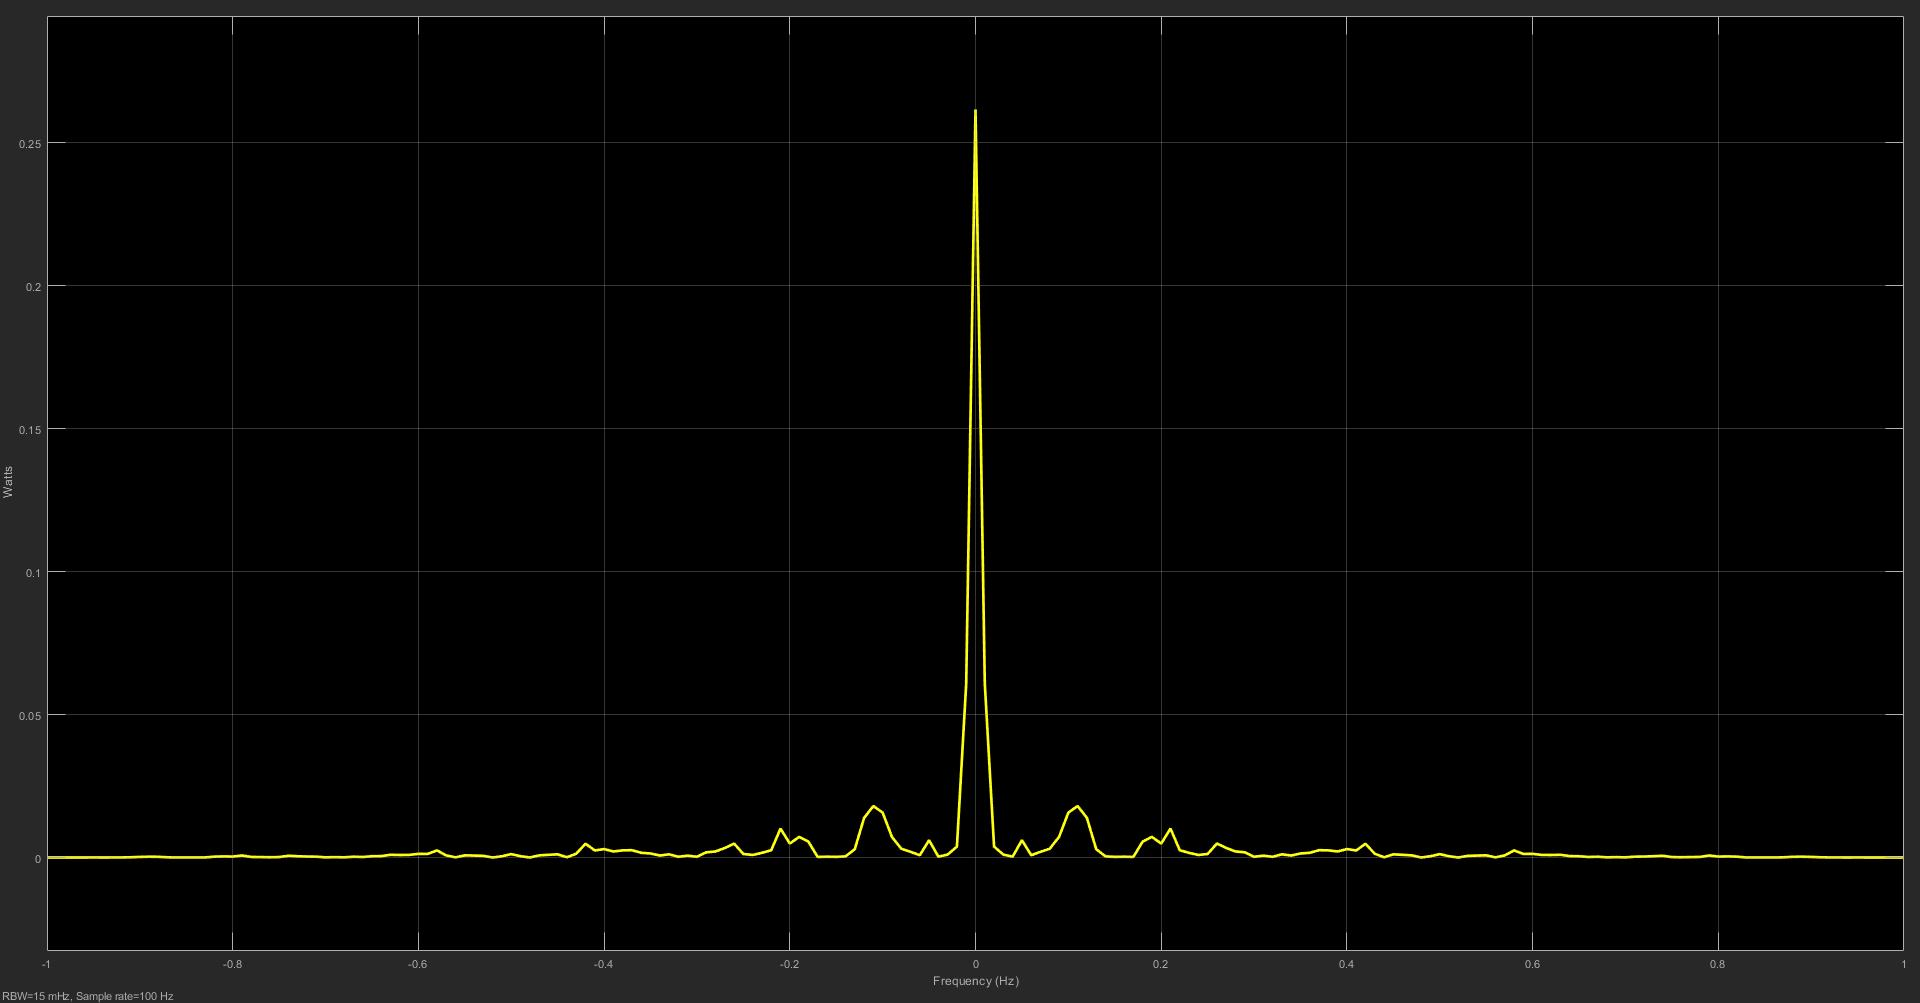
\includegraphics[width = \linewidth]{OO_Rect_F_Spectrum.jpg}
  \caption{Spectrum for On-Off encoding with a Full Width Rectangle Shaped Pulse}
  \label{fig:OO-Rect-F-Spectrum}
\end{figure}
\begin{figure}[H]
  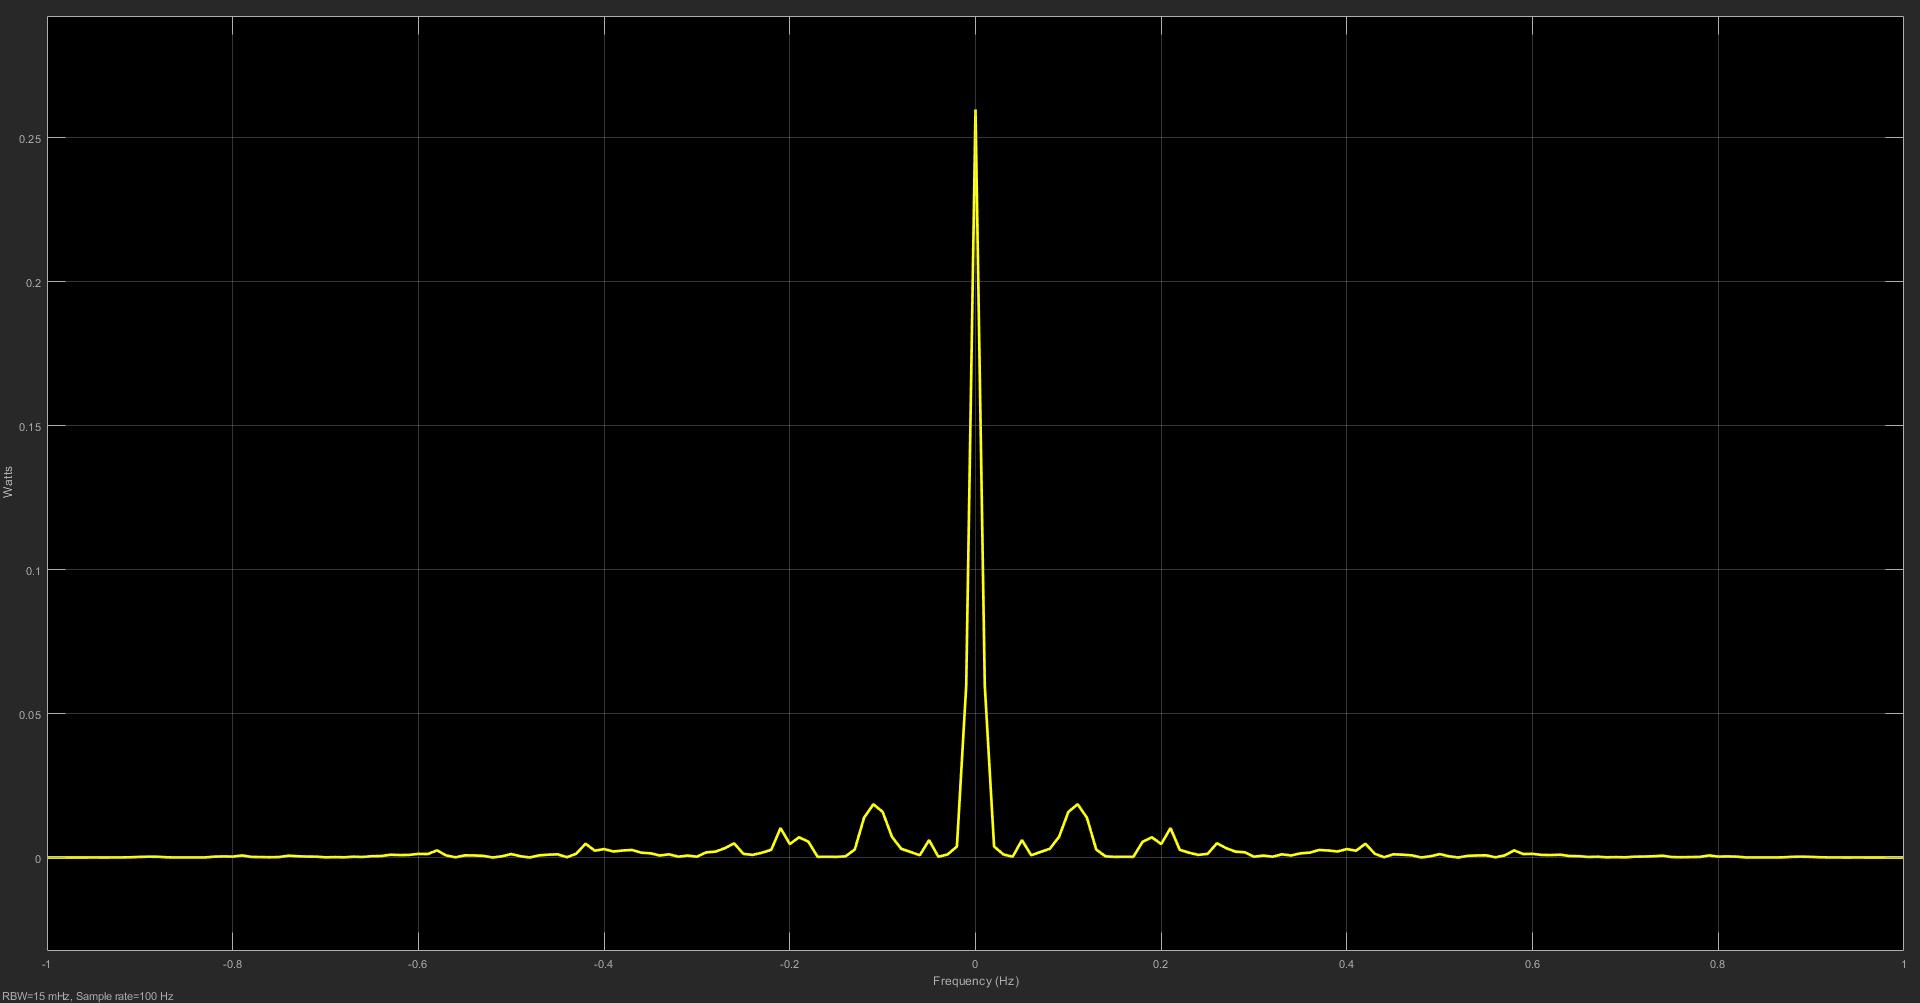
\includegraphics[width = \linewidth]{OO_Rect_H_Spectrum.jpg}
  \caption{Spectrum for On-Off encoding with a Half Width Rectangle Shaped Pulse}
  \label{fig:OO-Rect-H-Spectrum}
\end{figure}
\begin{figure}[H]
  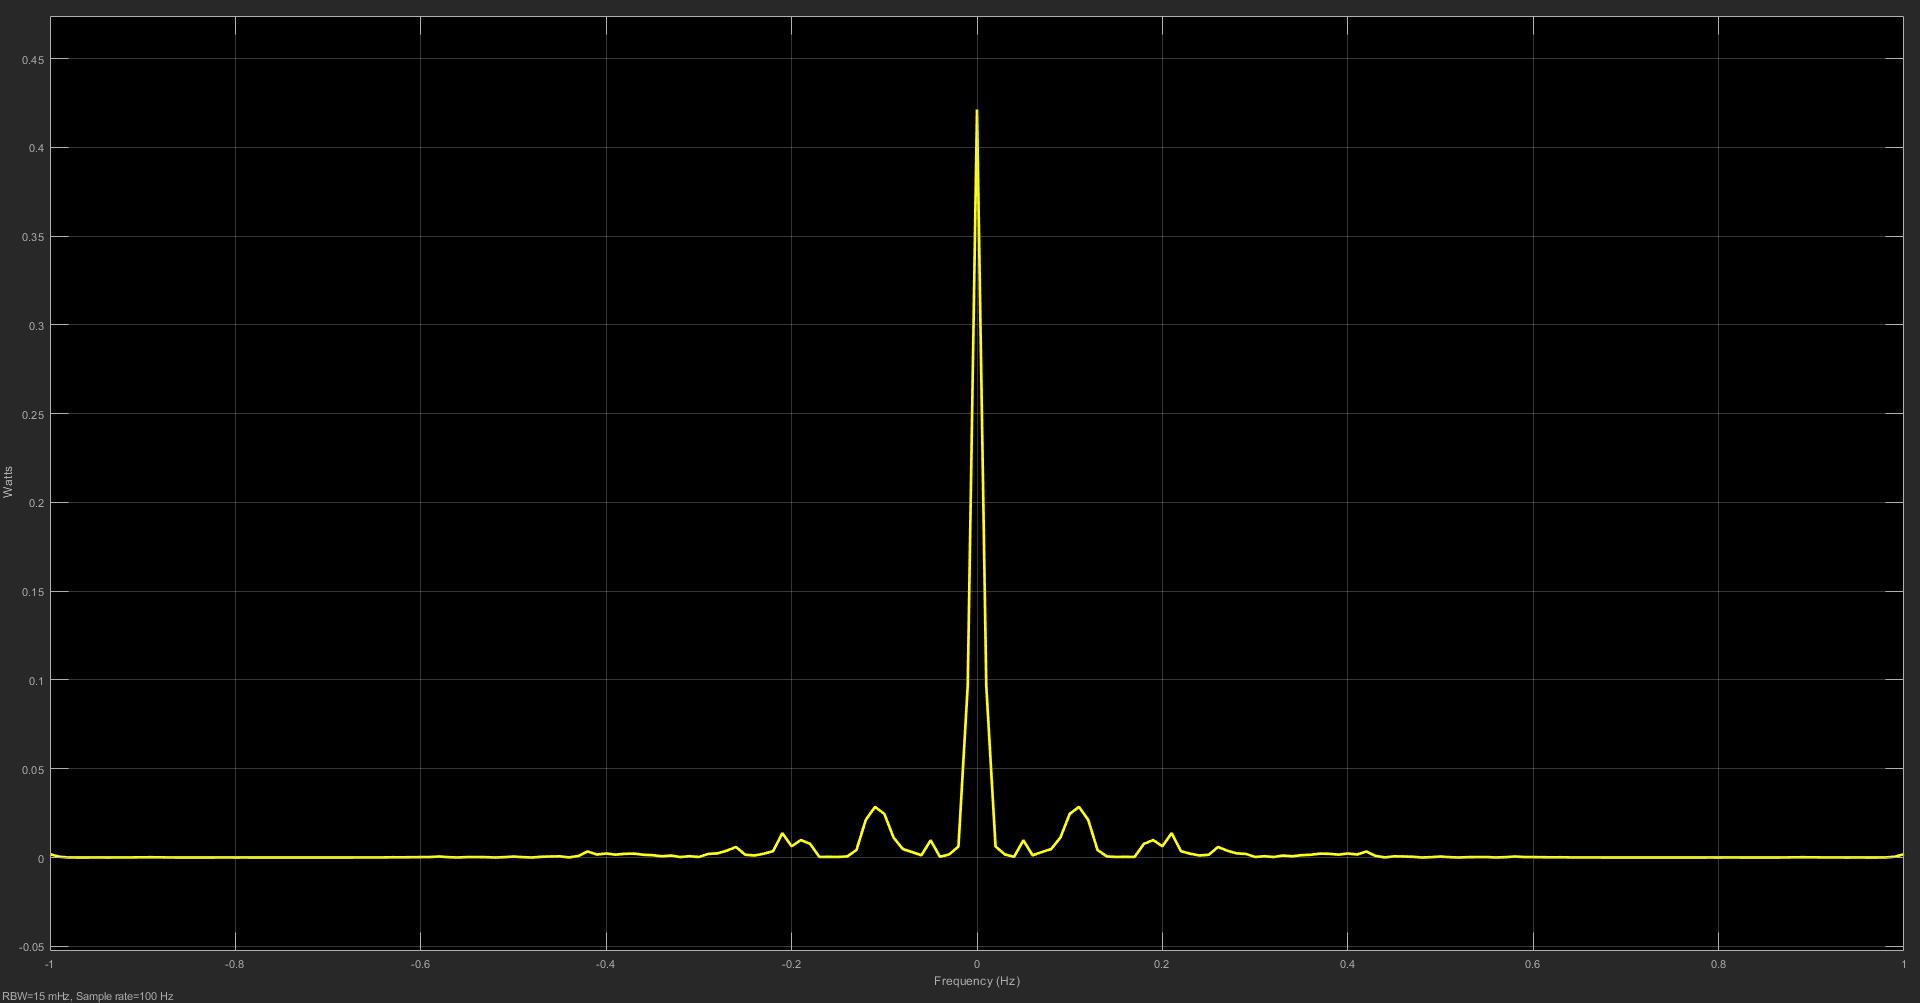
\includegraphics[width = \linewidth]{OO_Sin_Spectrum.jpg}
  \caption{Spectrum for On-Off encoding with a Sin Shaped Pulse}
  \label{fig:OO-Sin-Spectrum}
\end{figure}
\begin{figure}[H]
  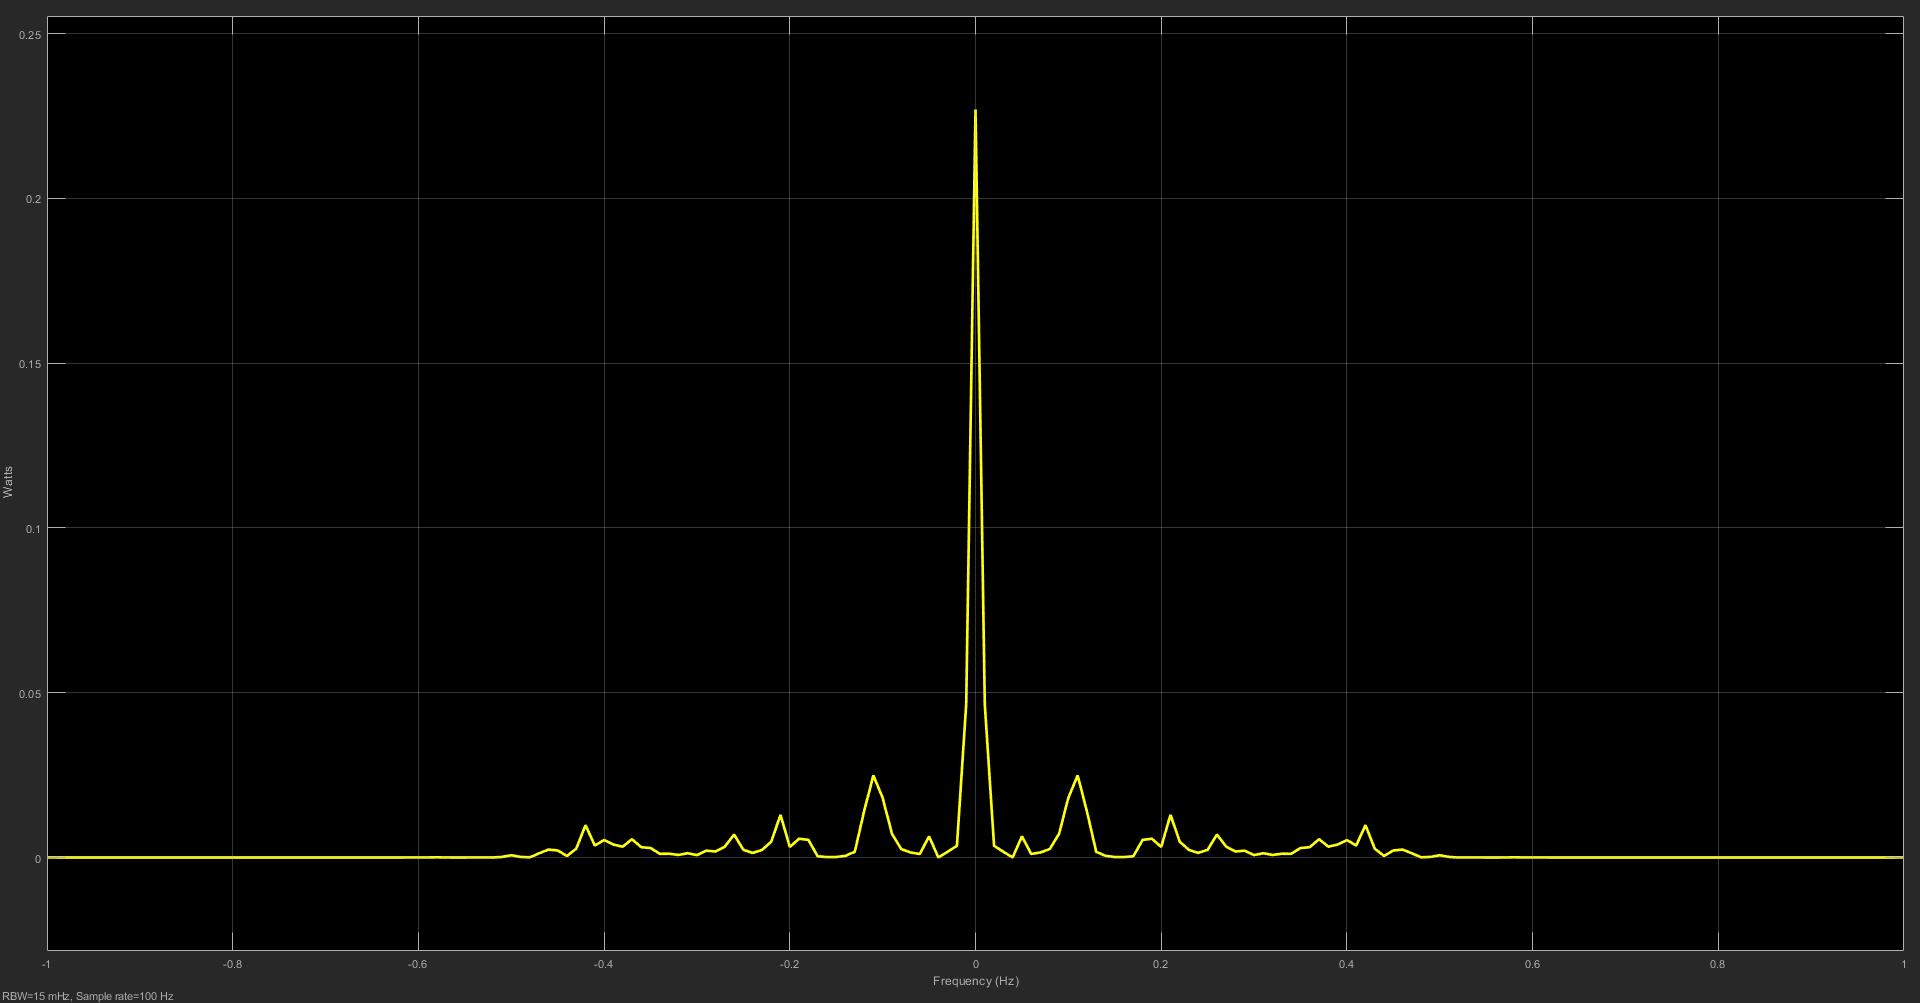
\includegraphics[width = \linewidth]{OO_Sinc_Spectrum.jpg}
  \caption{Spectrum for On-Off encoding with a Sinc Shaped Pulse}
  \label{fig:OO-Sinc-Spectrum}
\end{figure}
\begin{figure}[H]
  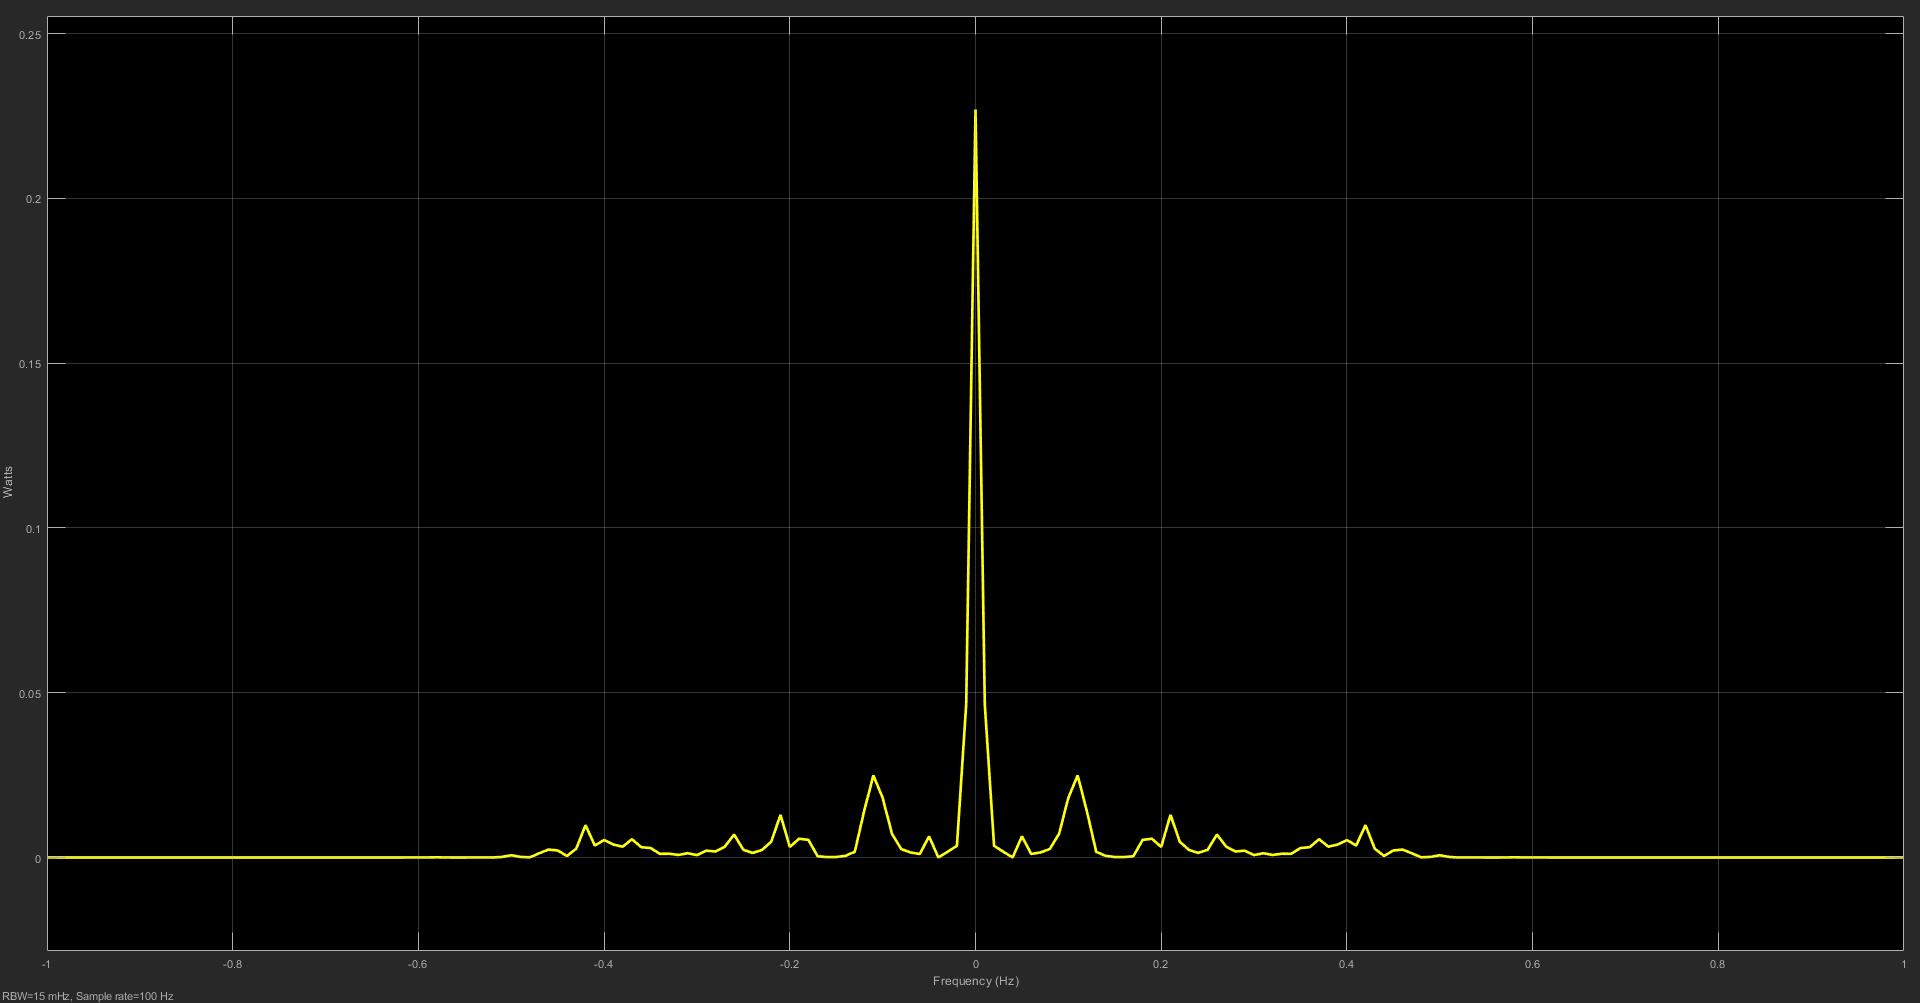
\includegraphics[width = \linewidth]{OO_Squared_Spectrum.jpg}
  \caption{Spectrum for On-Off encoding with a Sinc Squared Shaped Pulse}
  \label{fig:OO-Squared-Spectrum}
\end{figure}
\begin{figure}[H]
  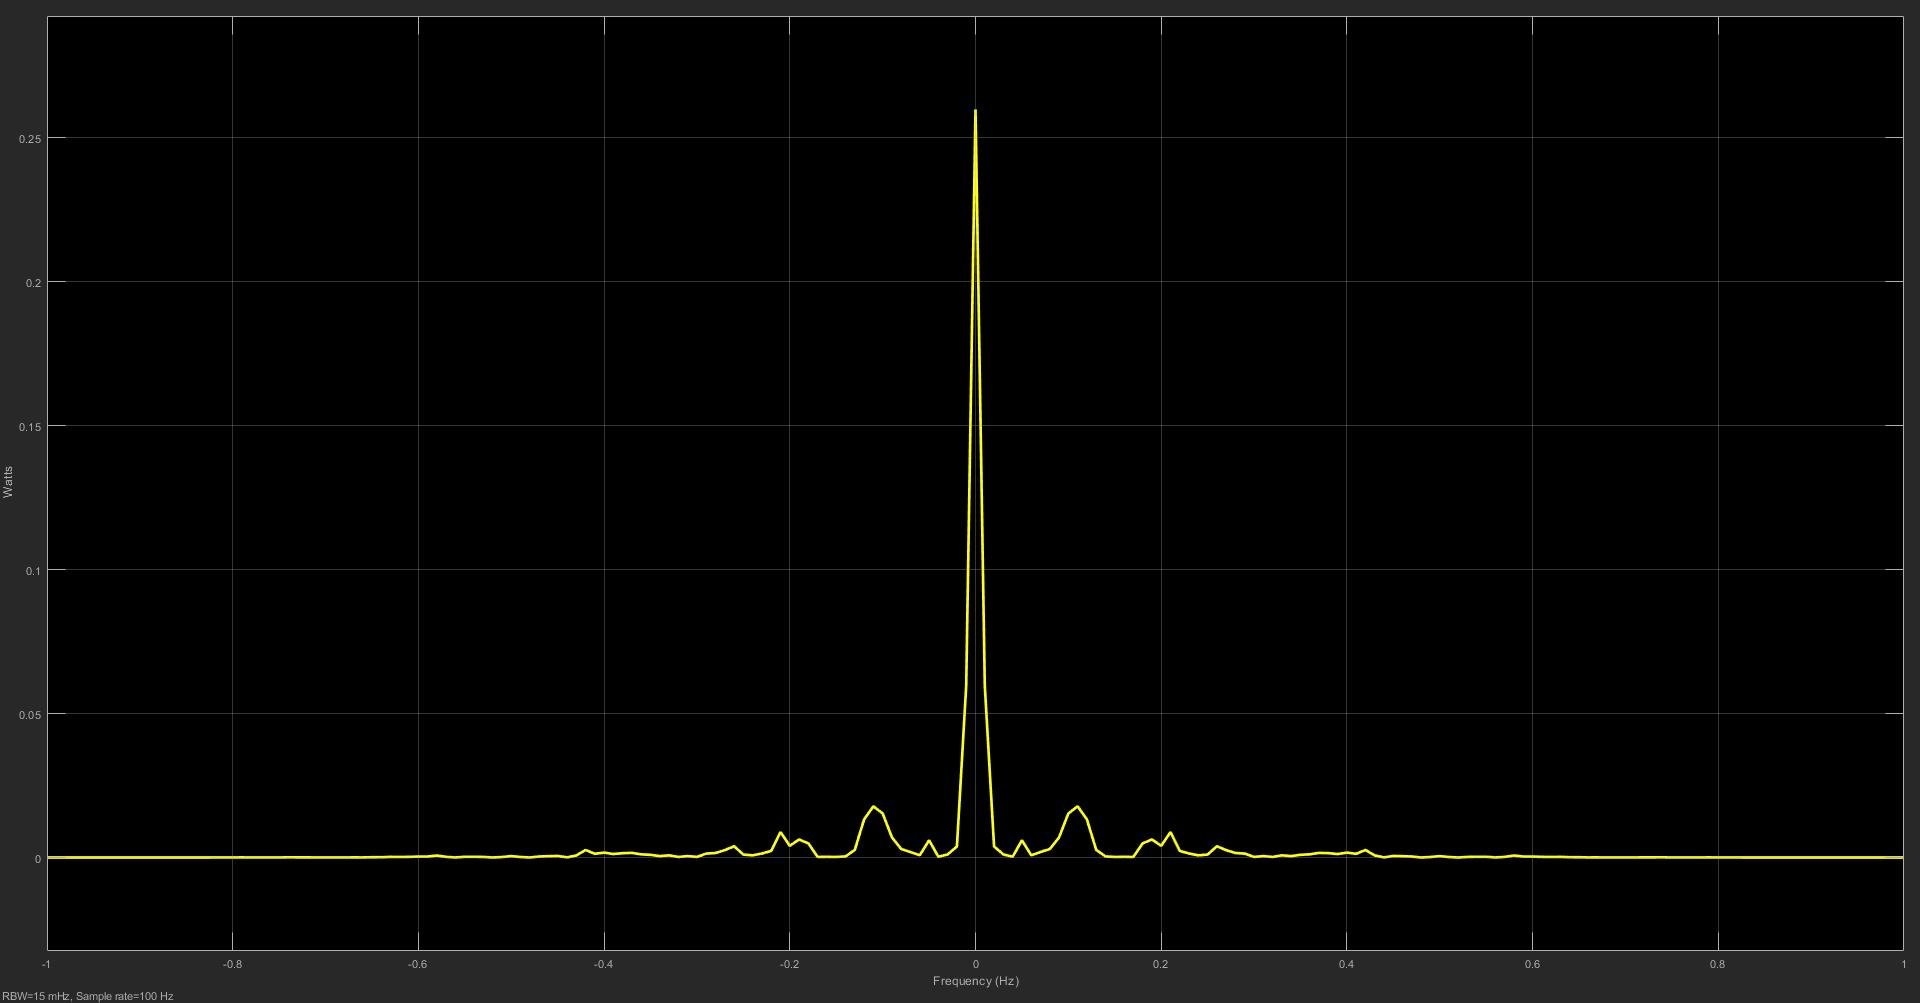
\includegraphics[width = \linewidth]{OO_Tri_F_Spectrum.jpg}
  \caption{Spectrum for On-Off encoding with a Full Width Triangle Shaped Pulse}
  \label{fig:OO-Tri-F-Spectrum}
\end{figure}
\begin{figure}[H]
  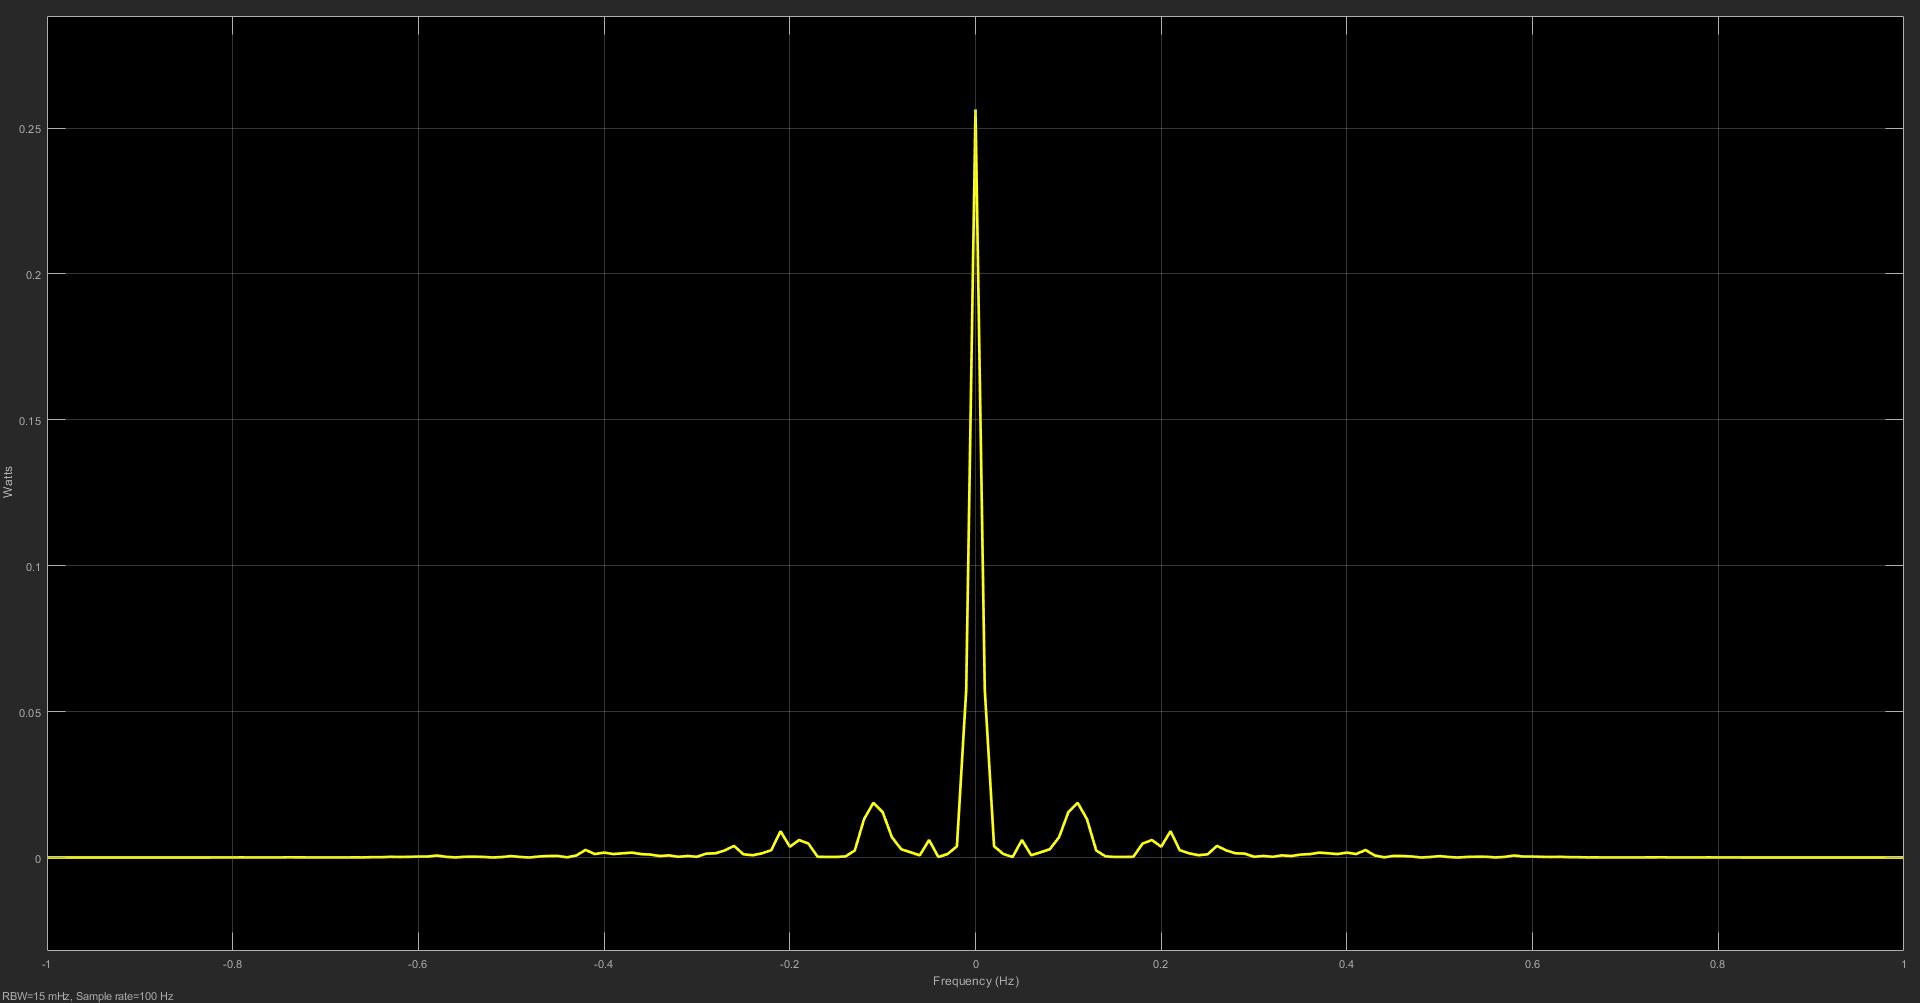
\includegraphics[width = \linewidth]{OO_Tri_H_Spectrum.jpg}
  \caption{Spectrum for On-Off encoding with a Half Width Triangle Shaped Pulse}
  \label{fig:OO-Tri-H-Spectrum}
\end{figure}
\subsection{Polar}
\subsubsection{Time Signal}
The following images or for Polar encoding with the various pulse shapes. They
are presented with the Polar encoded binary stream, the generated signal when
convoluted with a shaped pulse and the received signal with noise in the channel.
\begin{figure}[H]
  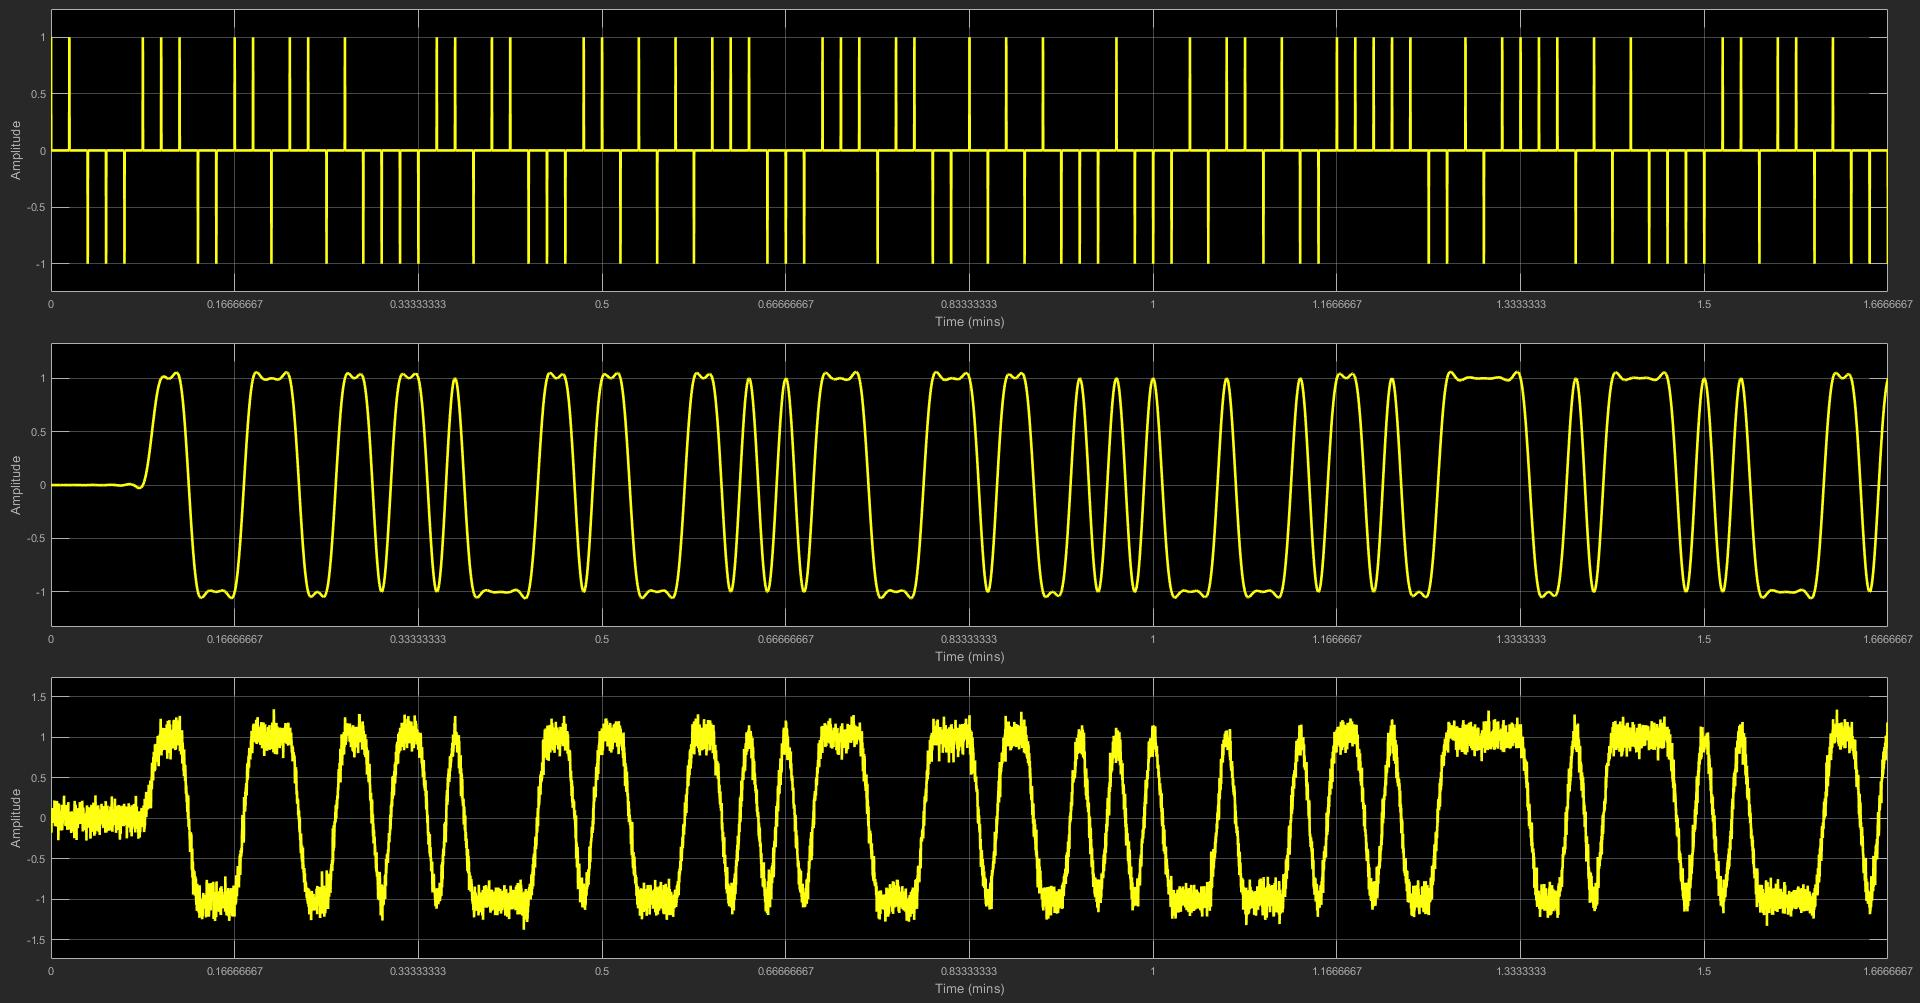
\includegraphics[width = \linewidth]{Polar_Raised.jpg}
  \caption{On-Off encoding with a Raised Cosine Shaped Pulse}
  \label{fig:Polar-Raised}
\end{figure}
\begin{figure}[H]
  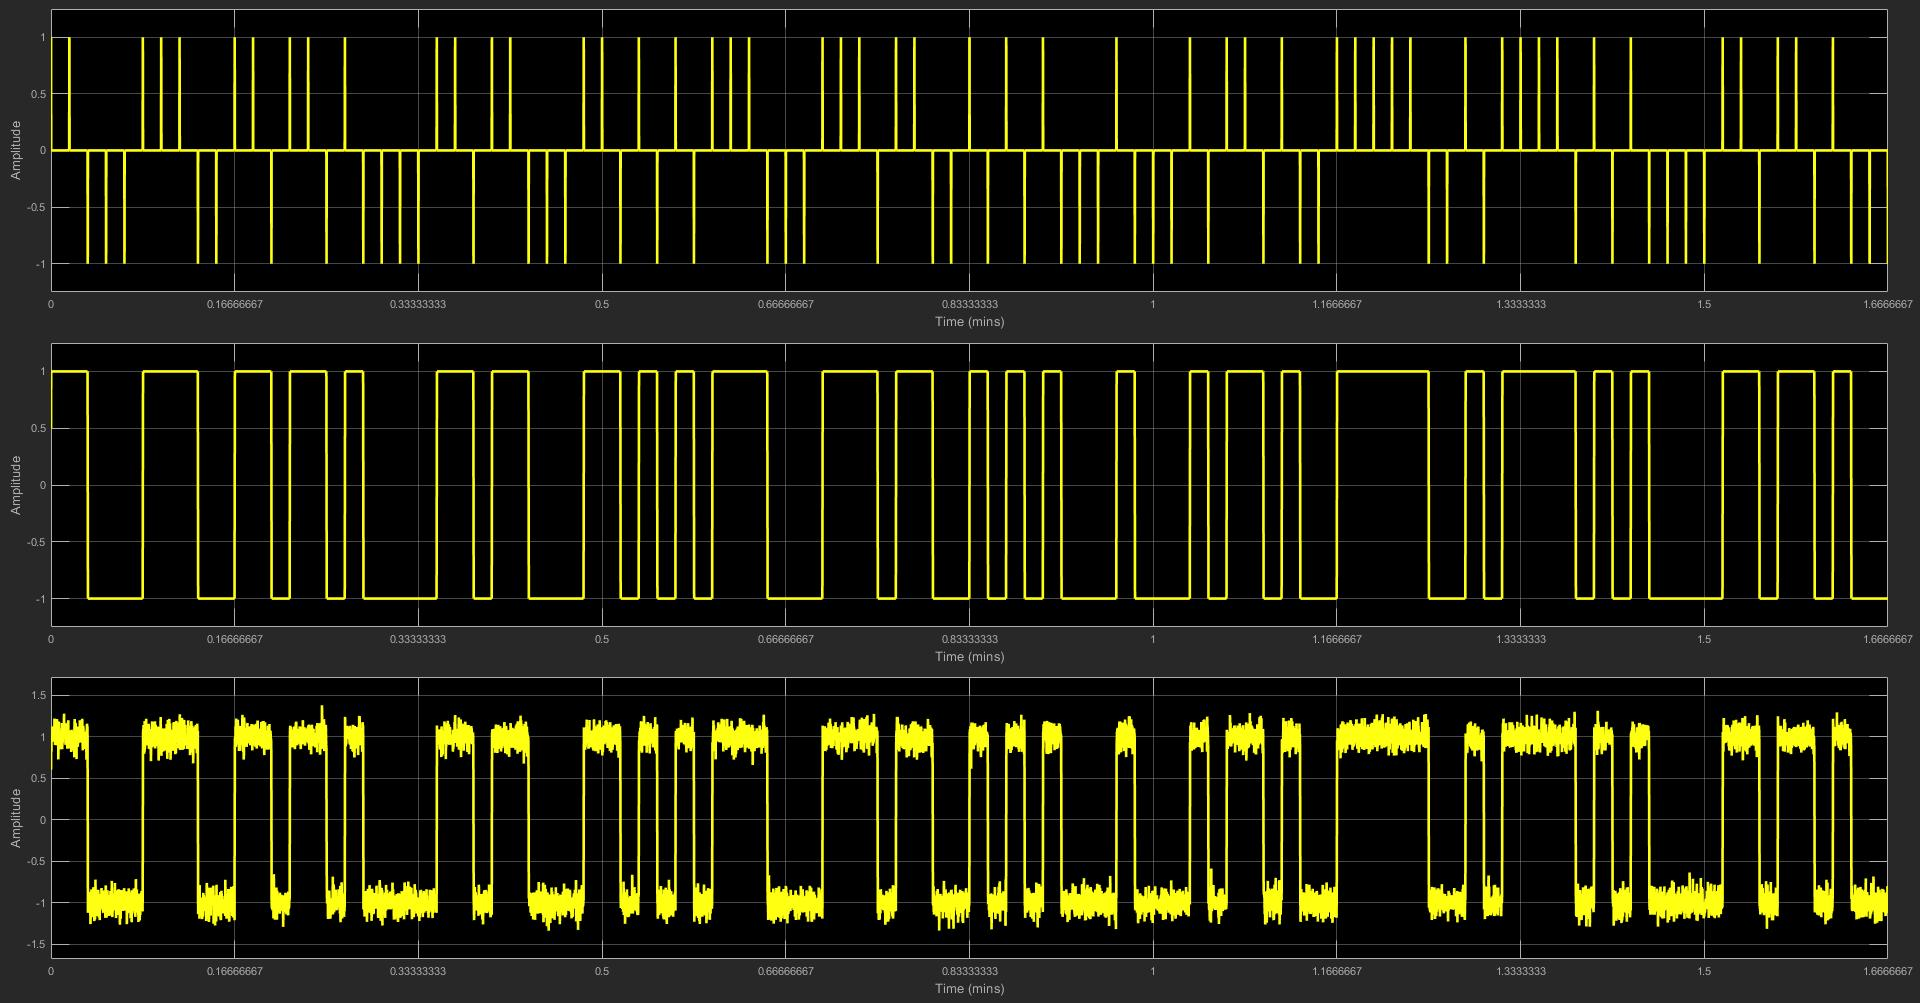
\includegraphics[width = \linewidth]{Polar_Rect_F.jpg}
  \caption{On-Off encoding with a Full Width Rectangle Shaped Pulse}
  \label{fig:Polar-Rect-F}
\end{figure}
\begin{figure}[H]
  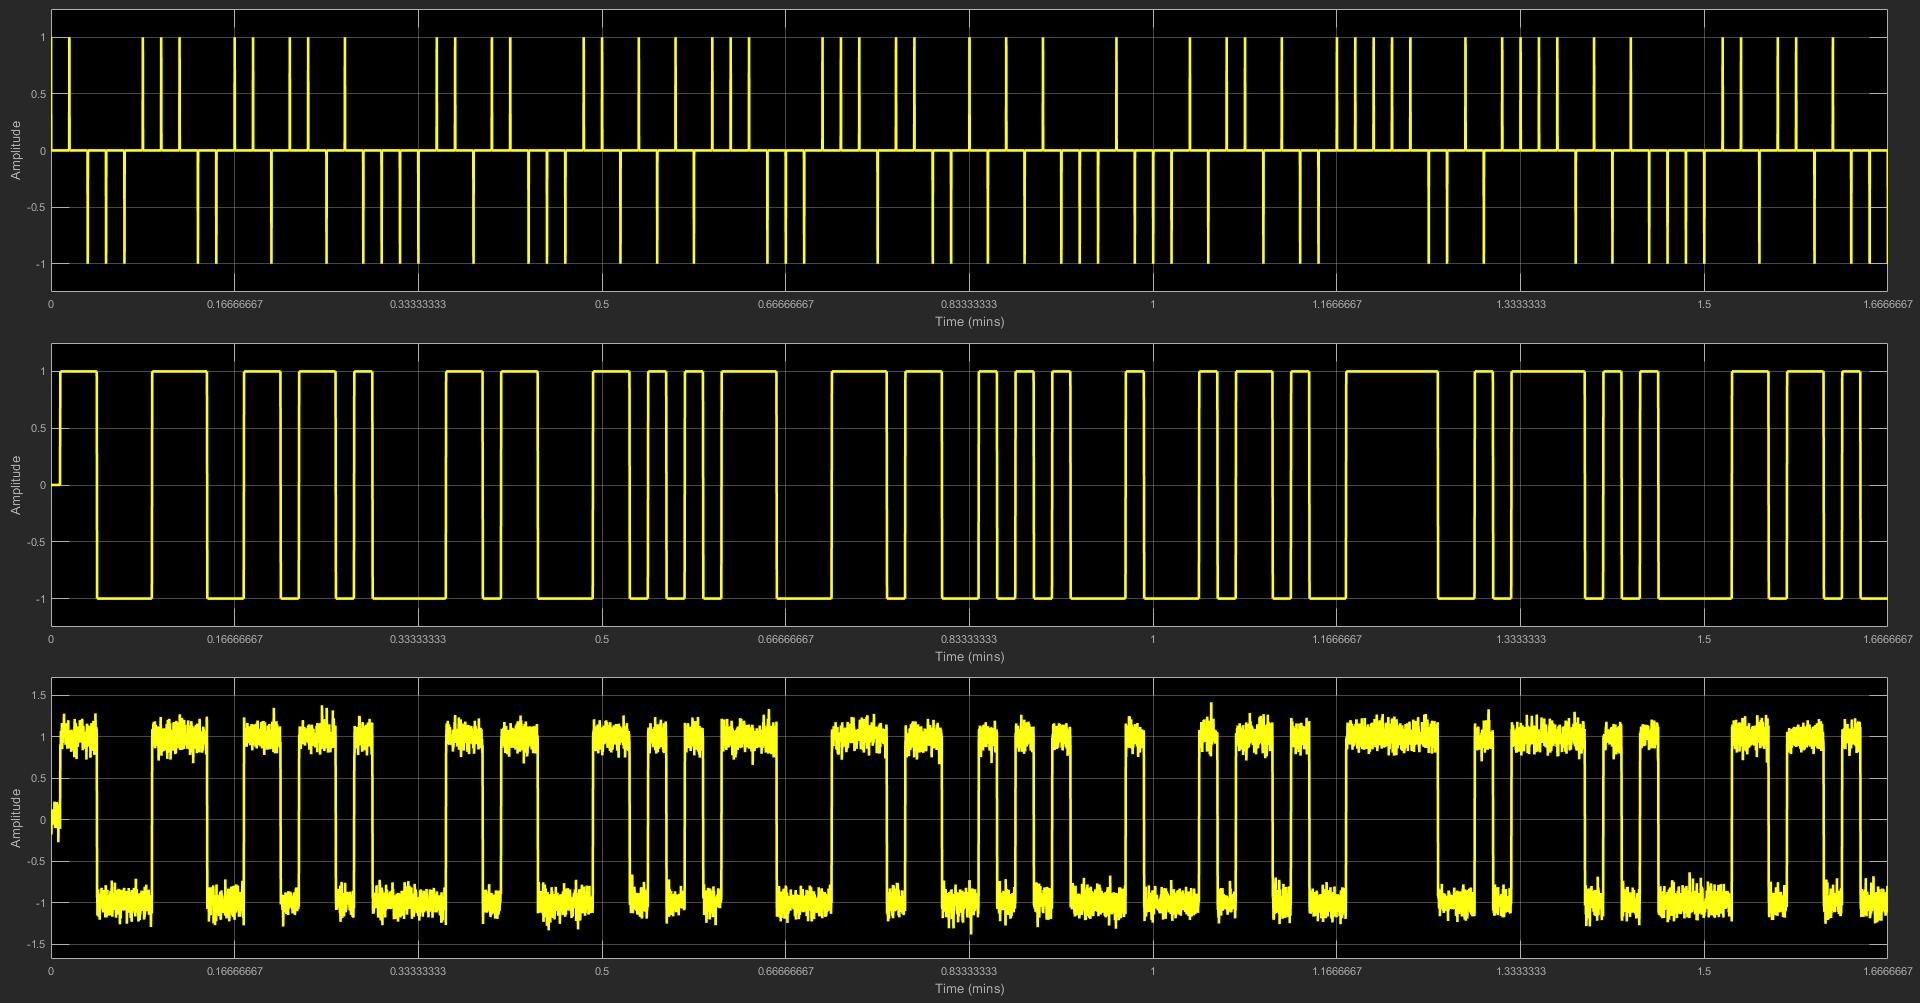
\includegraphics[width = \linewidth]{Polar_Rect_H.jpg}
  \caption{On-Off encoding with a Half Width Rectangle Shaped Pulse}
  \label{fig:Polar-Rect-H}
\end{figure}
\begin{figure}[H]
  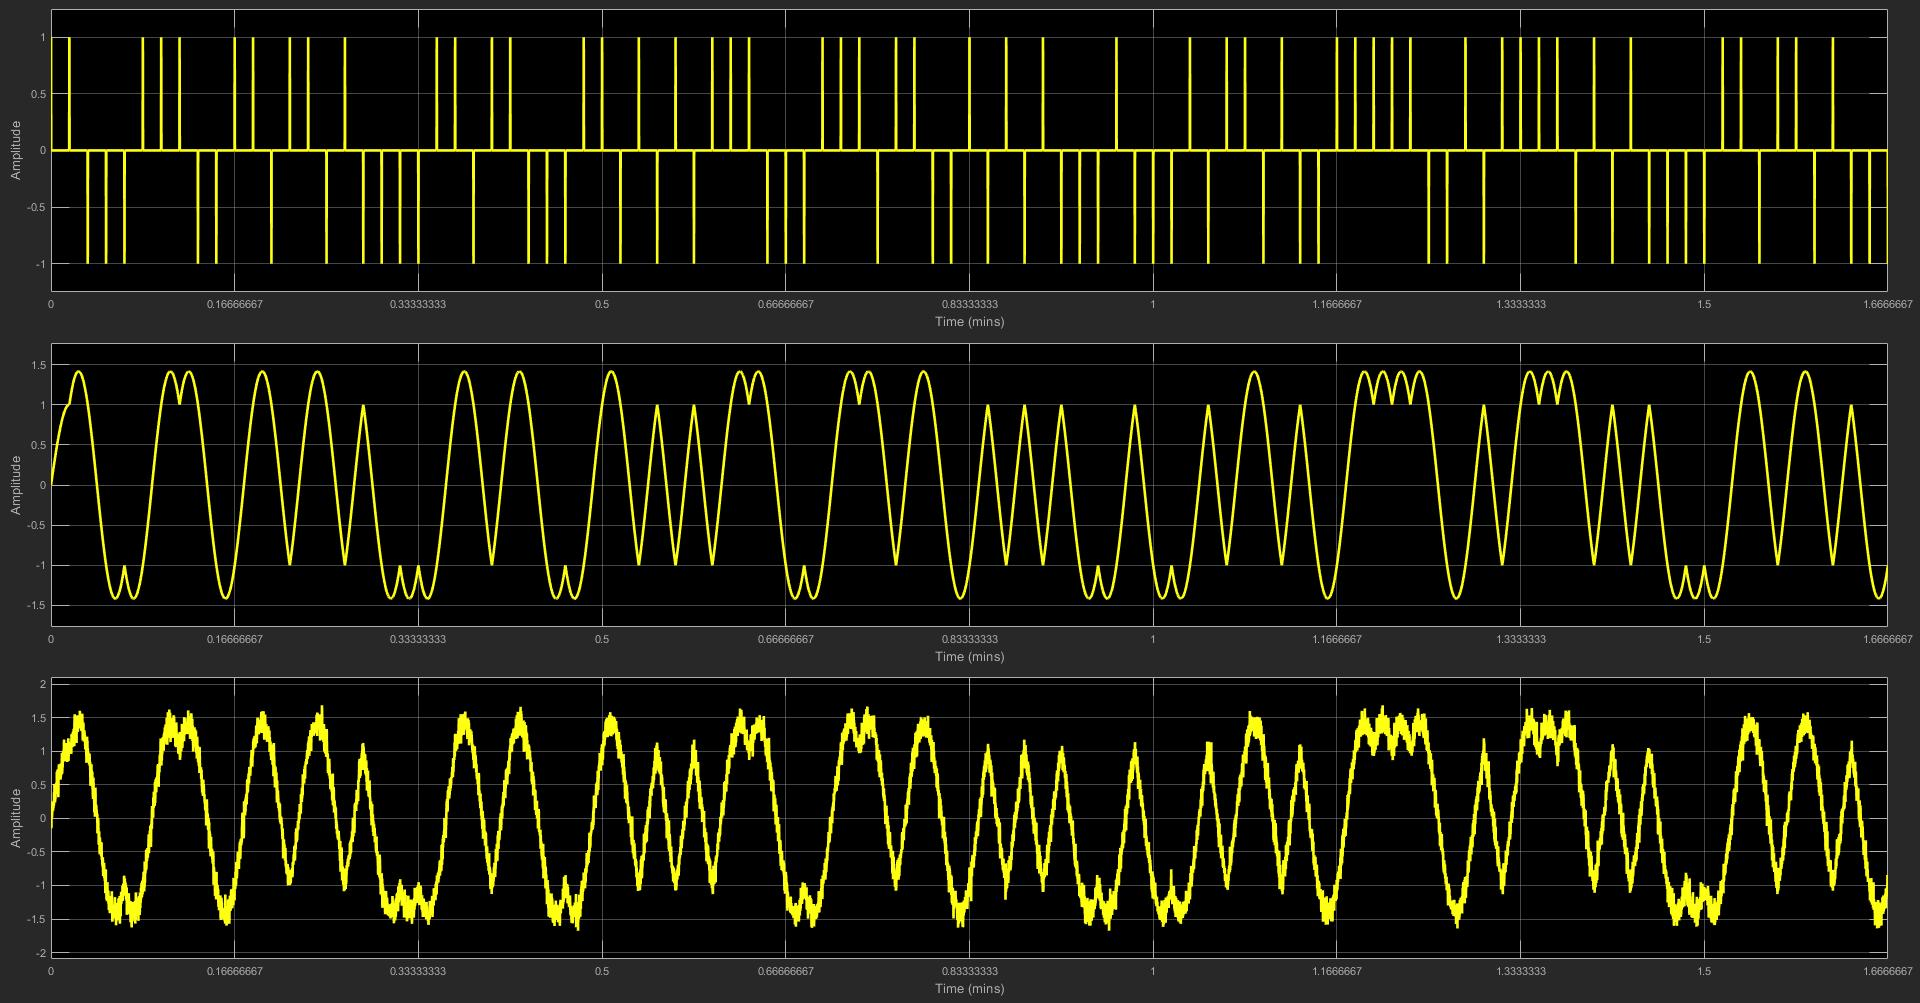
\includegraphics[width = \linewidth]{Polar_Sin.jpg}
  \caption{On-Off encoding with a Full Width Rectangle Shaped Pulse}
  \label{fig:Polar-Sin}
\end{figure}
\begin{figure}[H]
  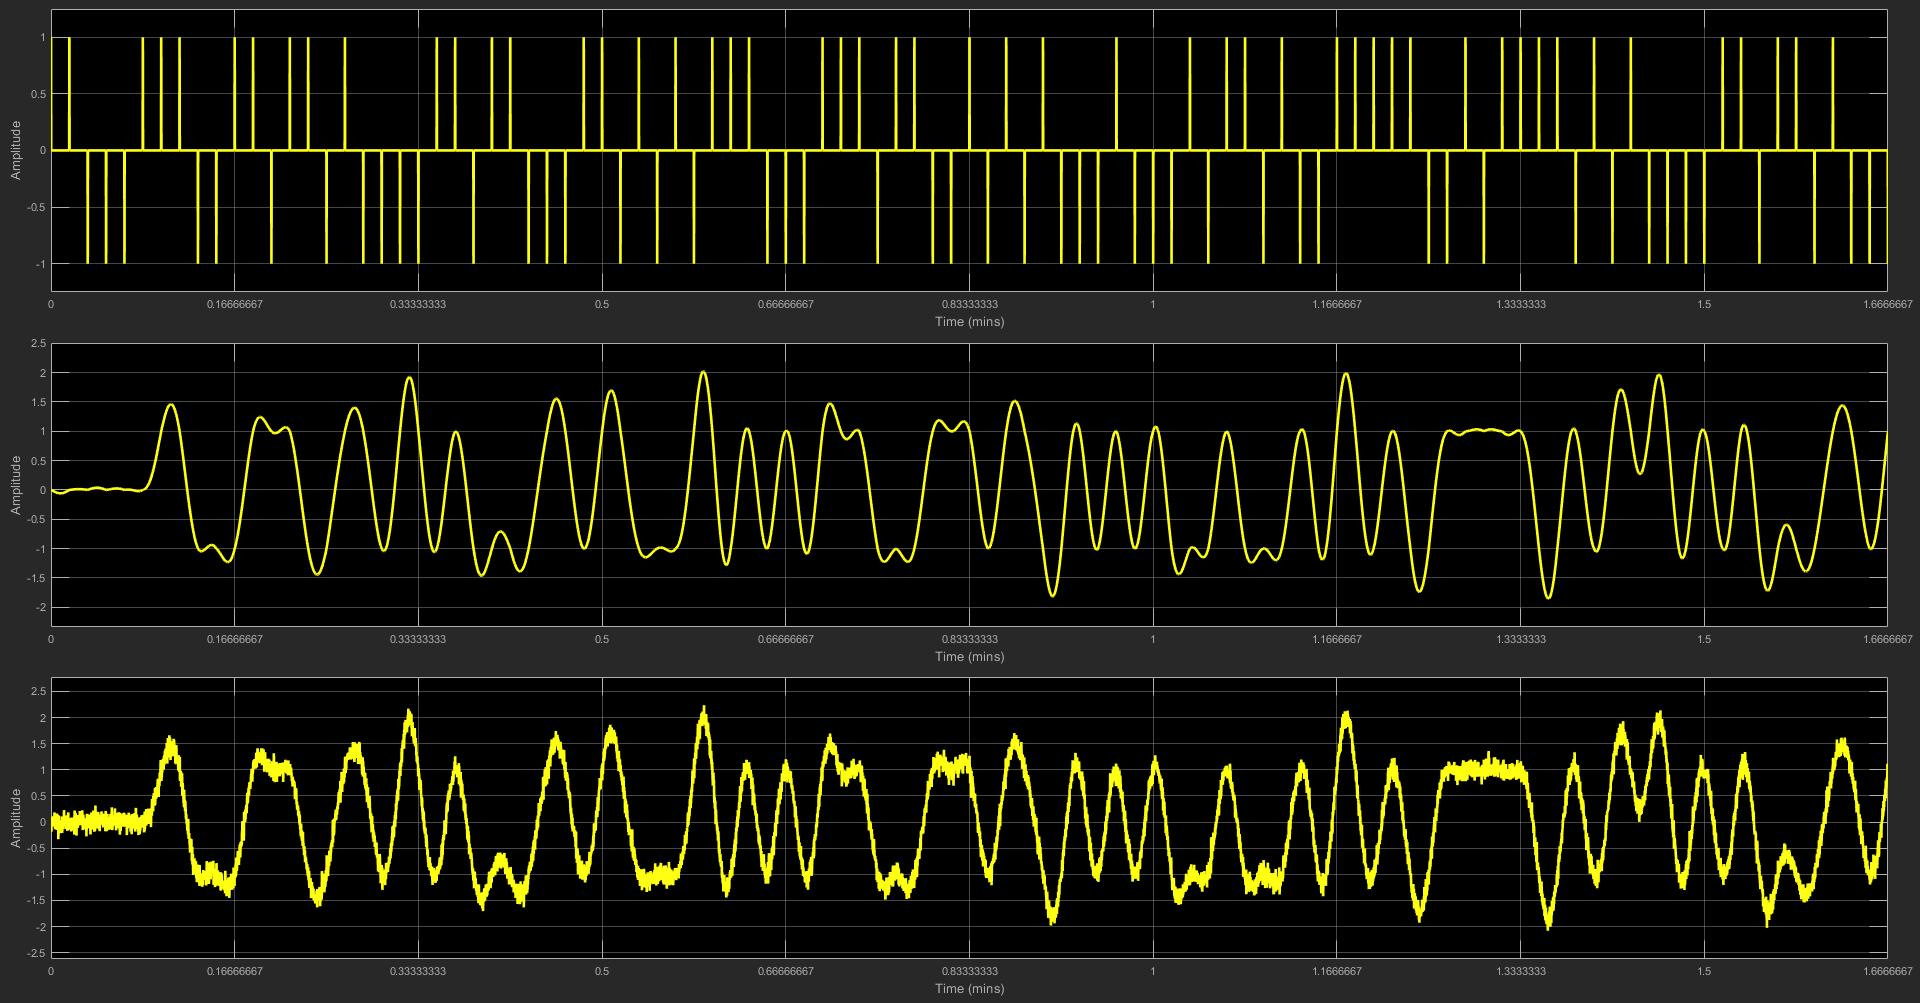
\includegraphics[width = \linewidth]{Polar_Sinc.jpg}
  \caption{On-Off encoding with a Sinc Shaped Pulse}
  \label{fig:Polar-Sinc}
\end{figure}
\begin{figure}[H]
  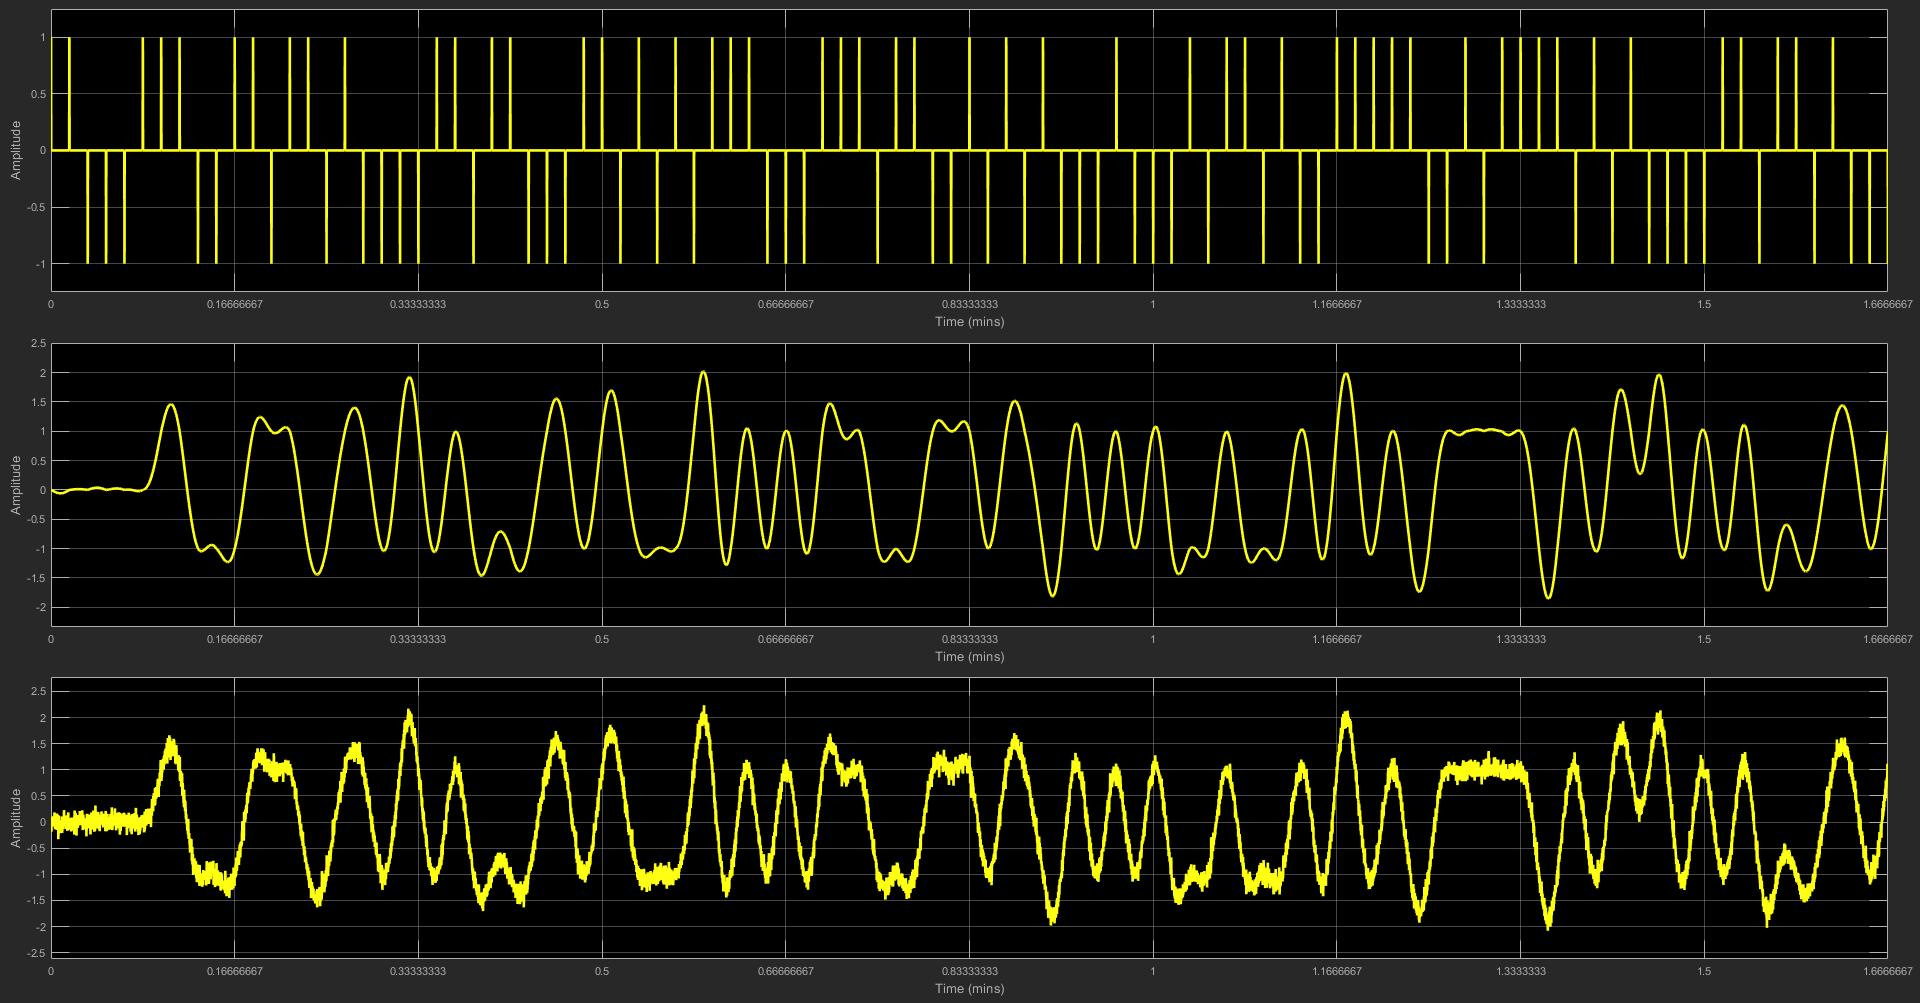
\includegraphics[width = \linewidth]{Polar_Squared.jpg}
  \caption{On-Off encoding with a Sinc Squared Shaped Pulse}
  \label{fig:Polar-Squared}
\end{figure}
\begin{figure}[H]
  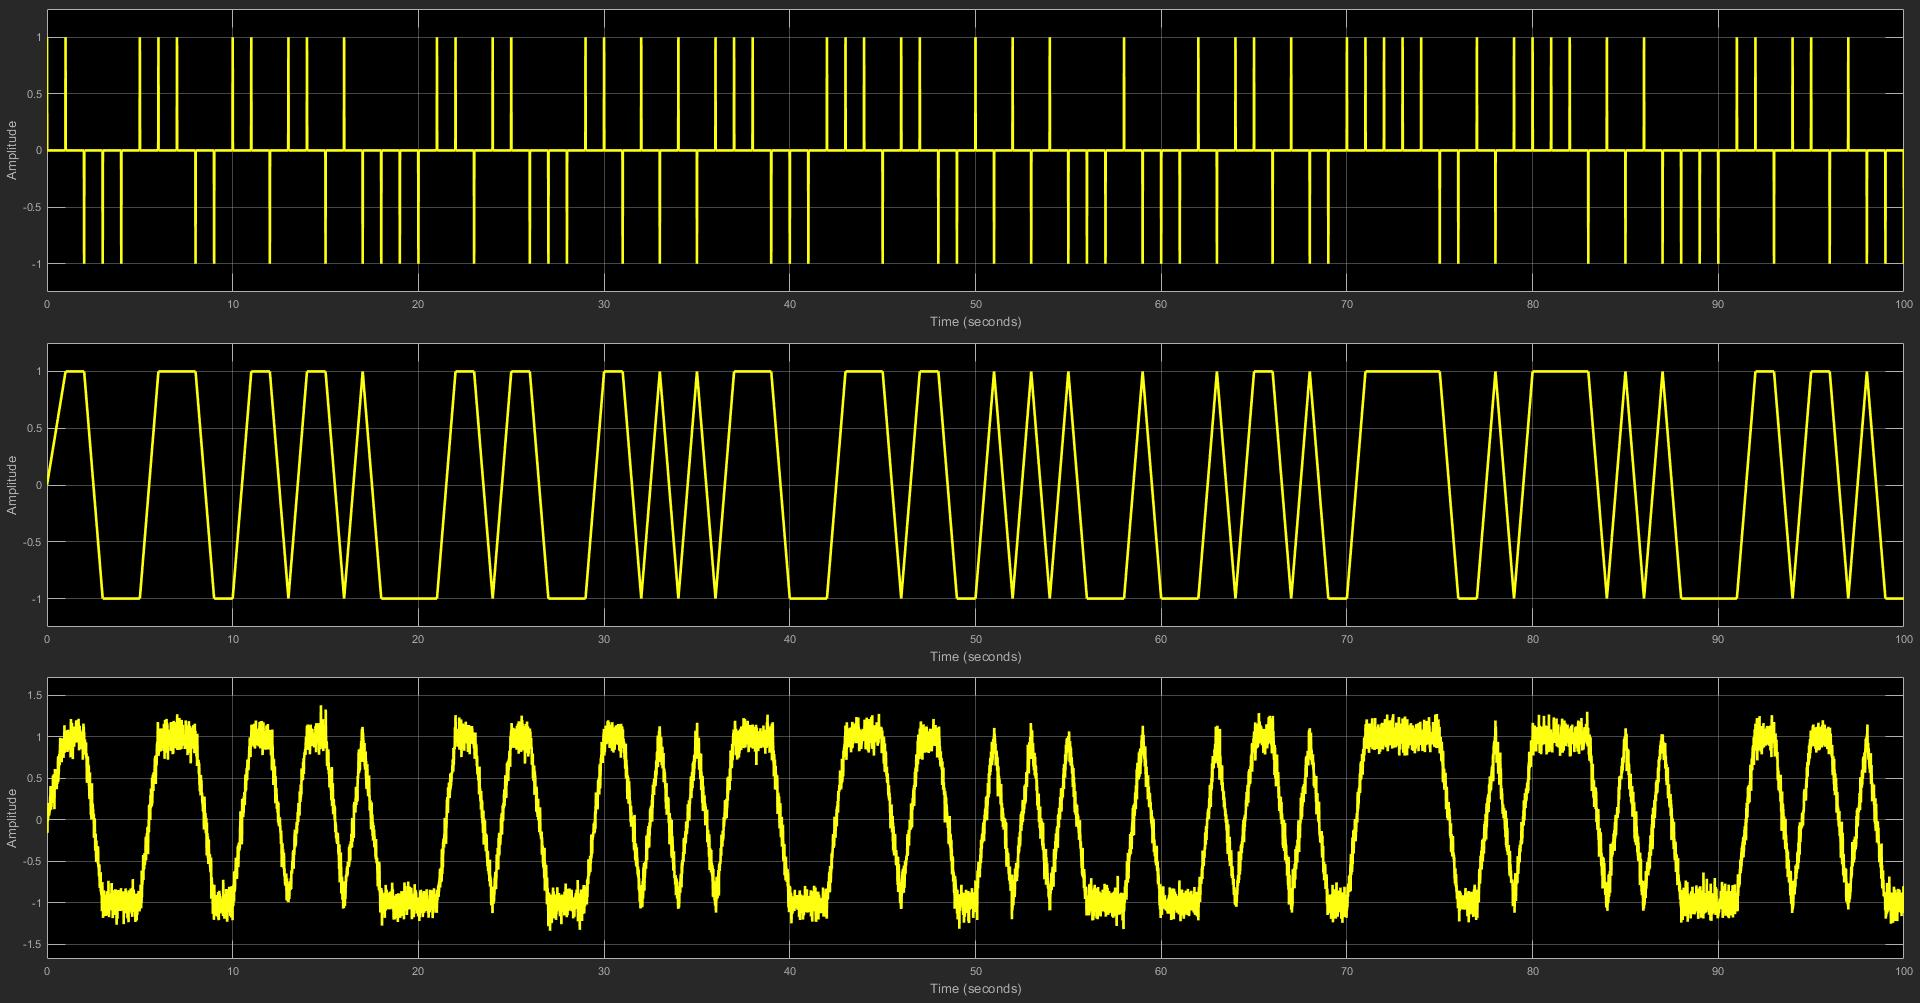
\includegraphics[width = \linewidth]{Polar_Tri_F.jpg}
  \caption{On-Off encoding with a Full Width Triangle Shaped Pulse}
  \label{fig:Polar-Tri-F}
\end{figure}
\begin{figure}[H]
  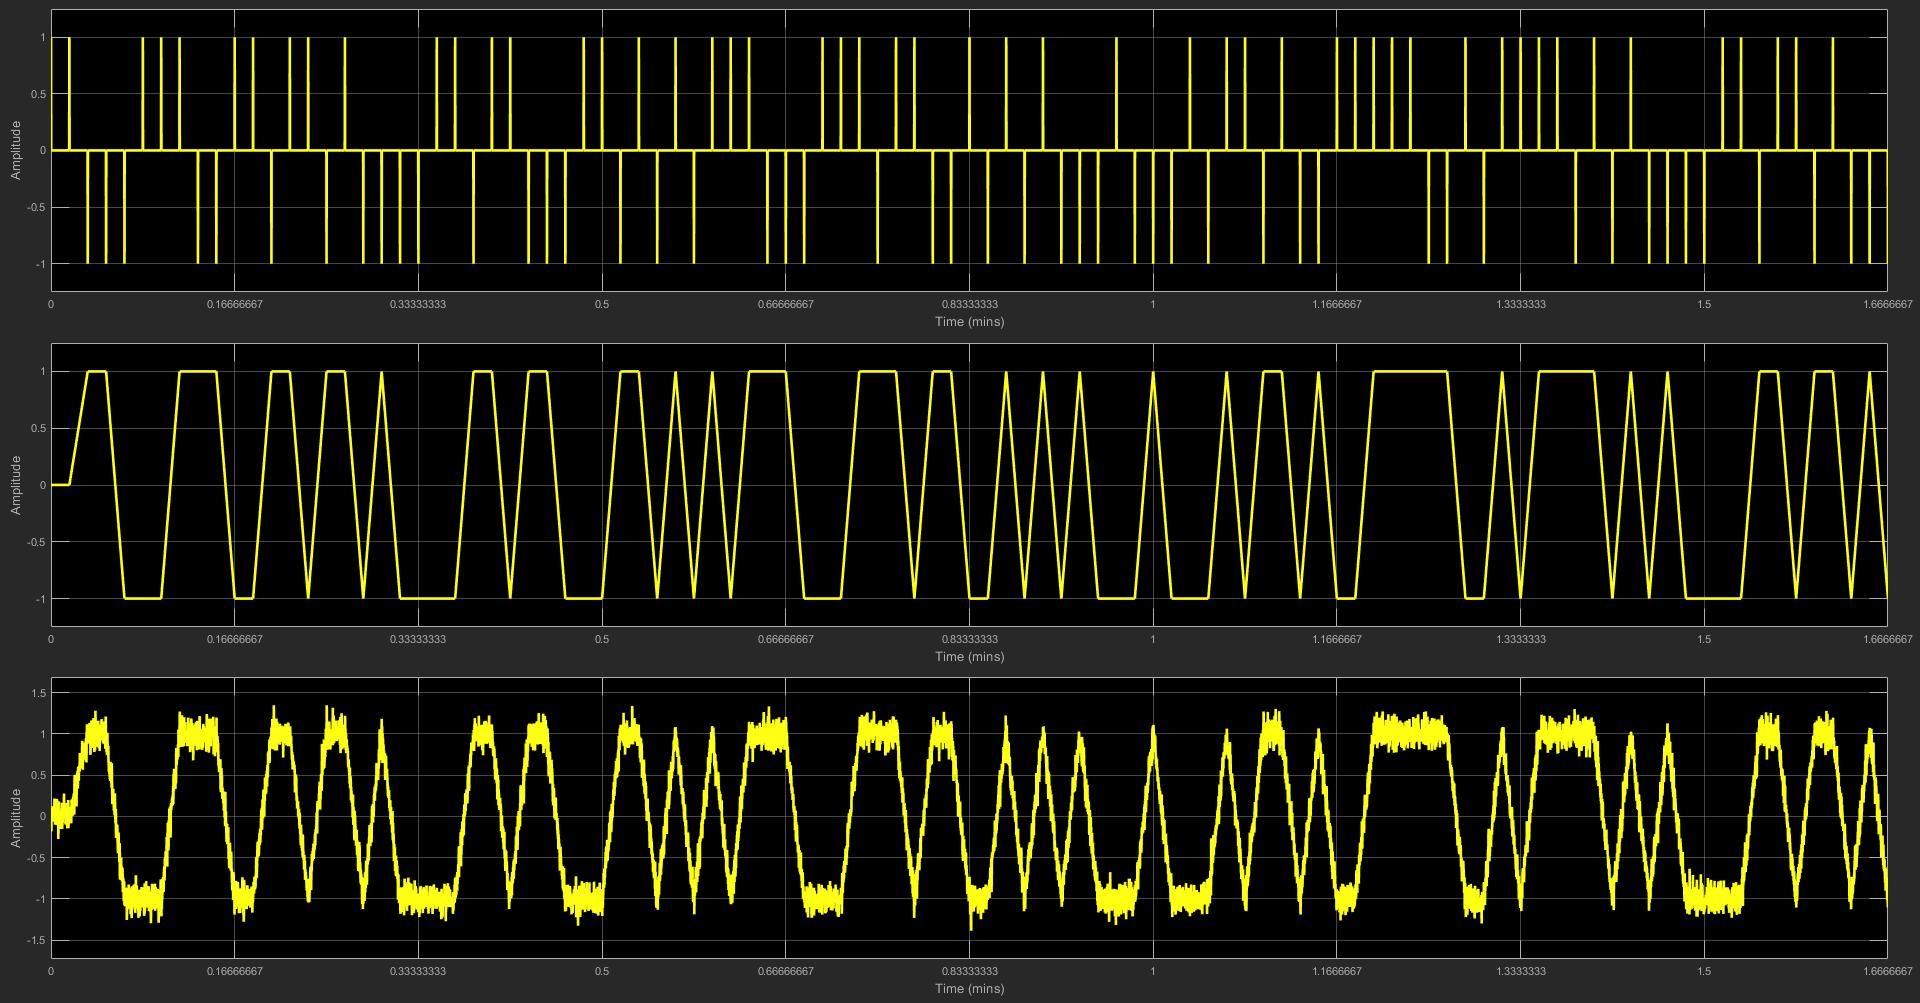
\includegraphics[width = \linewidth]{Polar_Tri_H.jpg}
  \caption{On-Off encoding with a Half Width Triangle Shaped Pulse}
  \label{fig:Polar-Tri-H}
\end{figure}
Something that should be noted is that the apparent difference between full width and half with shaped pulses for both Rectangle and Triangle shaped pulses have an identical waveform. The difference is the half width is a delayed signal.
\subsubsection{Eye Diagrams}
\begin{figure}[H]
  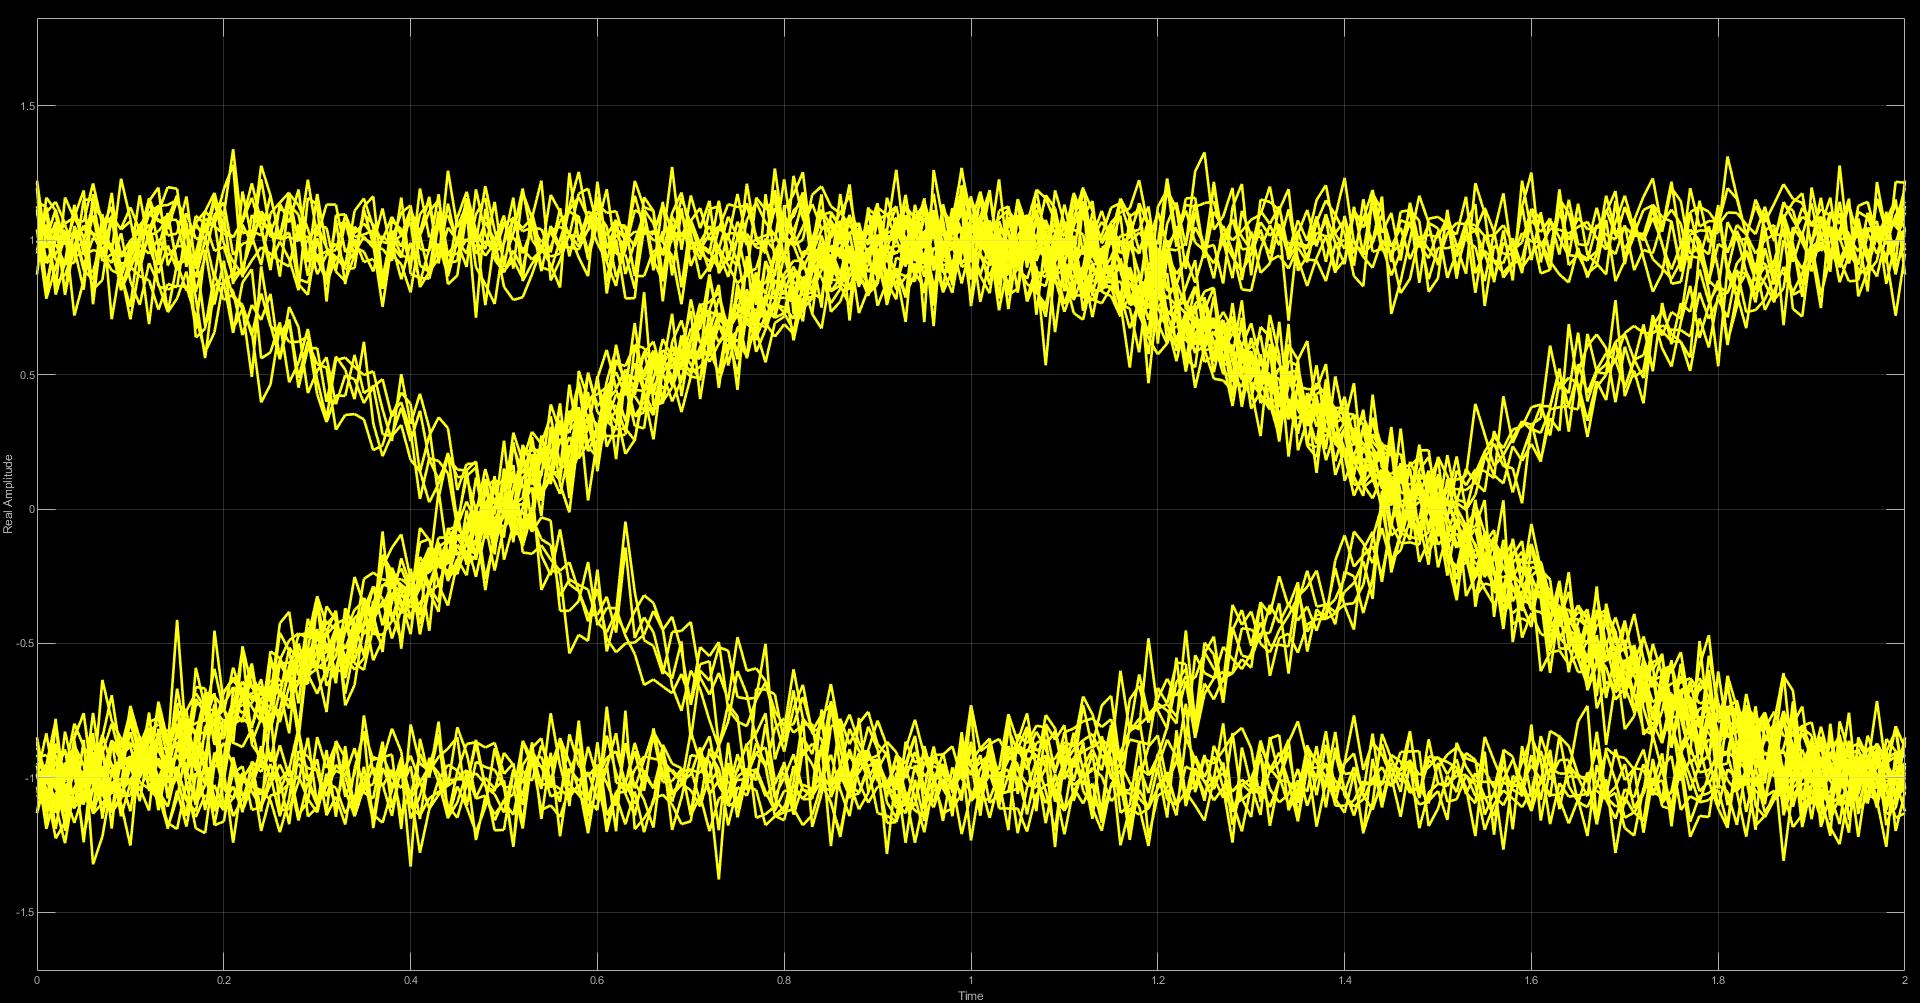
\includegraphics[width = \linewidth]{Polar_Raised_Eye.jpg}
  \caption{Eye Diagram for Polar encoding with a Raised Cosine Shaped Pulse}
  \label{fig:Polar-Raised-Eye}
\end{figure}
\begin{figure}[H]
  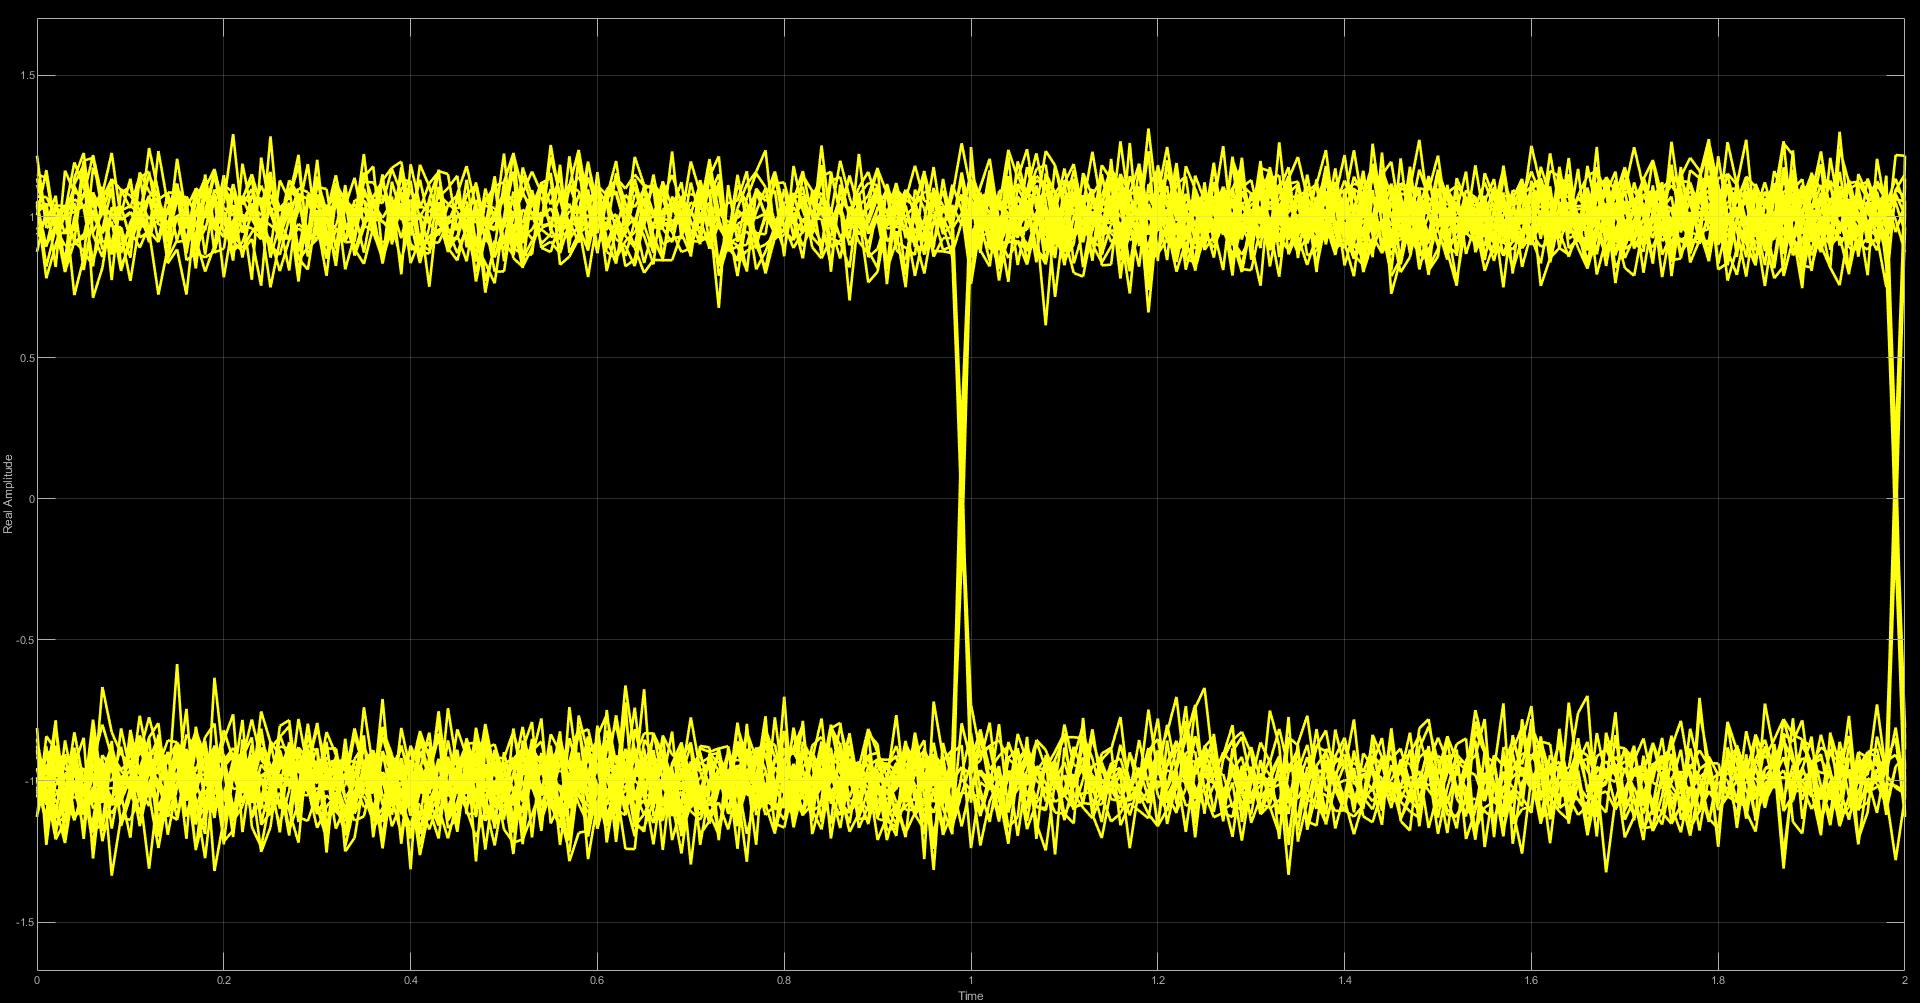
\includegraphics[width = \linewidth]{Polar_Rect_F_Eye.jpg}
  \caption{Eye Diagram for Polar encoding with a Full Width Rectangle Shaped Pulse}
  \label{fig:Polar-Rect-F-Eye}
\end{figure}
\begin{figure}[H]
  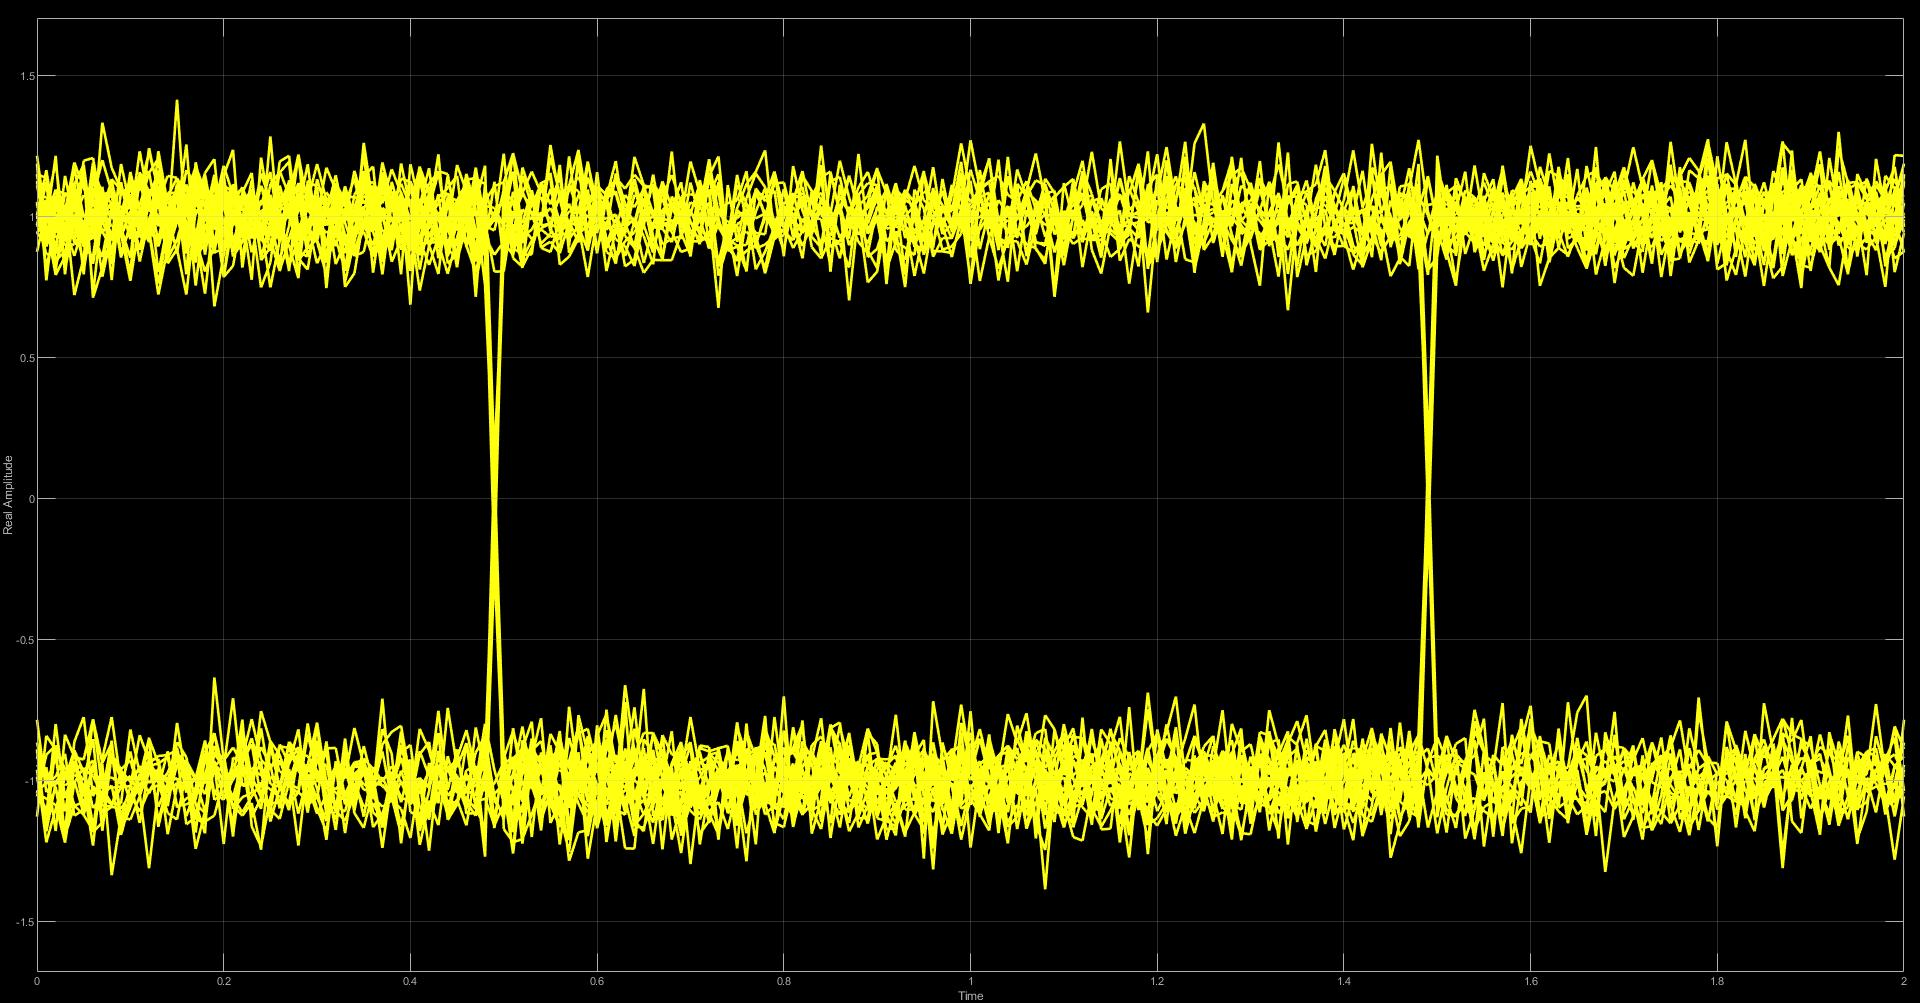
\includegraphics[width = \linewidth]{Polar_Rect_H_Eye.jpg}
  \caption{Eye Diagram for Polar encoding with a Half Width Rectangle Shaped Pulse}
  \label{fig:Polar-Rect-H-Eye}
\end{figure}
\begin{figure}[H]
  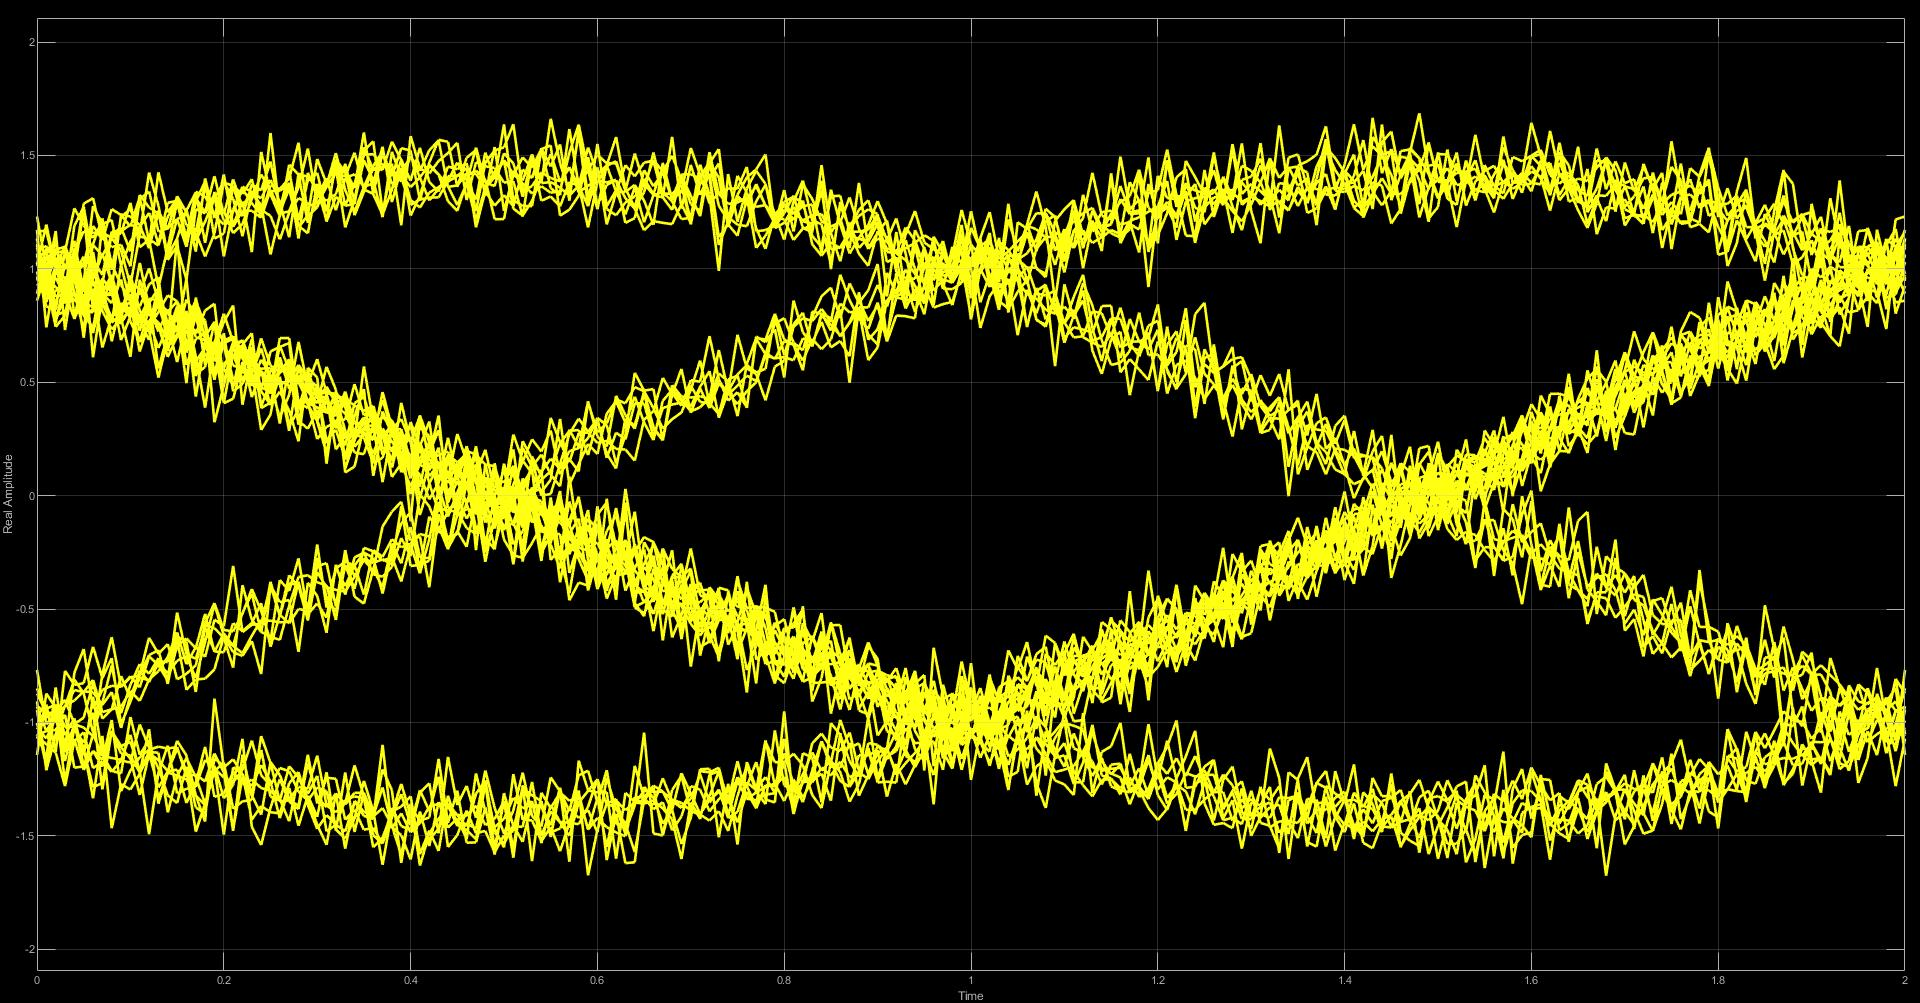
\includegraphics[width = \linewidth]{Polar_Sin_Eye.jpg}
  \caption{Eye Diagram for Polar encoding with a Full Width Rectangle Shaped Pulse}
  \label{fig:Polar-Sin-Eye}
\end{figure}
\begin{figure}[H]
  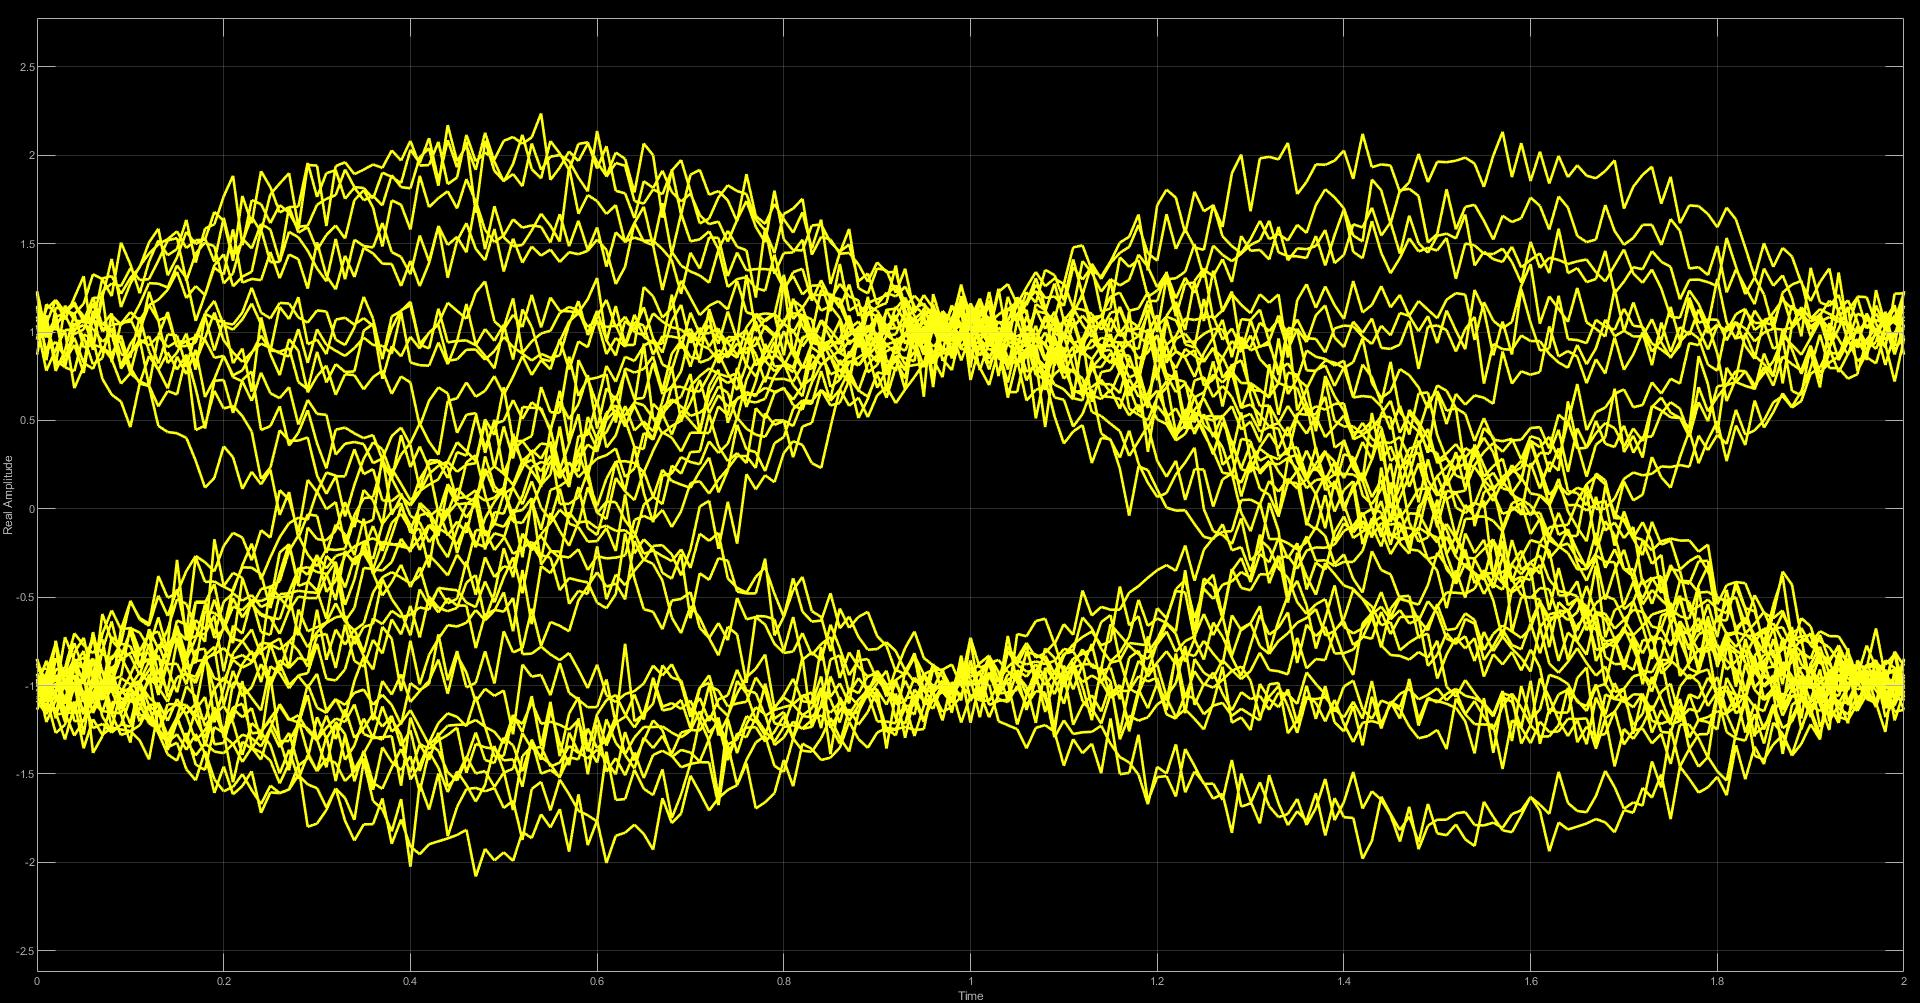
\includegraphics[width = \linewidth]{Polar_Sinc_Eye.jpg}
  \caption{Eye Diagram for Polar encoding with a Sinc Shaped Pulse}
  \label{fig:Polar-Sinc-Eye}
\end{figure}
\begin{figure}[H]
  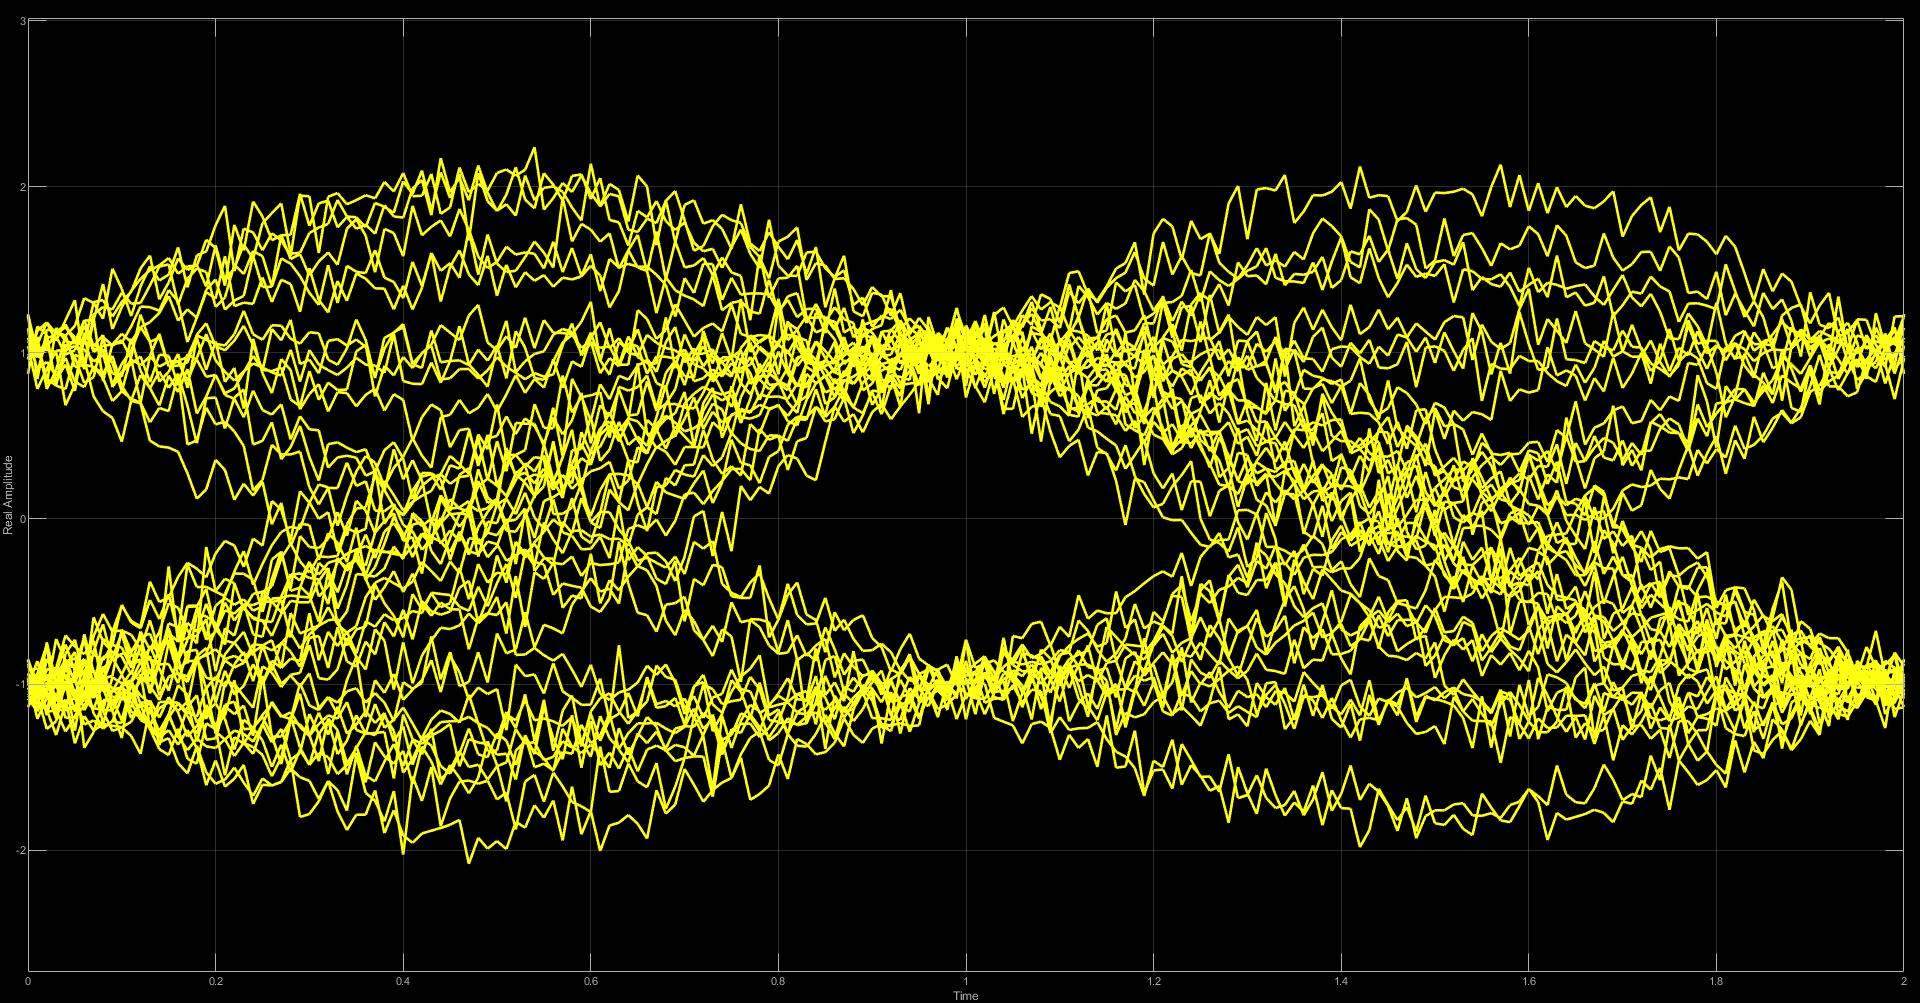
\includegraphics[width = \linewidth]{Polar_Squared_Eye.jpg}
  \caption{Eye Diagram for Polar encoding with a Sinc Squared Shaped Pulse}
  \label{fig:Polar-Squared-Eye}
\end{figure}
\begin{figure}[H]
  \includegraphics[width = \linewidth]{Polar_Tri_F_Eye.jpg}
  \caption{Eye Diagram for Polar encoding with a Full Width Triangle Shaped Pulse}
  \label{fig:Polar-Tri-F-Eye}
\end{figure}
\begin{figure}[H]
  \includegraphics[width = \linewidth]{Polar_Tri_H_Eye.jpg}
  \caption{Eye Diagram for Polar encoding with a Half Width Triangle Shaped Pulse}
  \label{fig:Polar-Tri-H-Eye}
\end{figure}
When looking at the eye diagrams, it can be seen in the full and half width rectangle pulses that in the half width shaped pulse the decision instant is offset by half the period of the signal.
\subsubsection{Spectrum}
\begin{figure}[H]
  \includegraphics[width = \linewidth]{Polar_Raised_Spectrum.jpg}
  \caption{Spectrum for Polar encoding with a Raised Cosine Shaped Pulse}
  \label{fig:Polar-Raised-Spectrum}
\end{figure}
\begin{figure}[H]
  \includegraphics[width = \linewidth]{Polar_Rect_F_Spectrum.jpg}
  \caption{Spectrum for Polar encoding with a Full Width Rectangle Shaped Pulse}
  \label{fig:Polar-Rect-F-Spectrum}
\end{figure}
\begin{figure}[H]
  \includegraphics[width = \linewidth]{Polar_Rect_H_Spectrum.jpg}
  \caption{Spectrum for Polar encoding with a Half Width Rectangle Shaped Pulse}
  \label{fig:Polar-Rect-H-Spectrum}
\end{figure}
\begin{figure}[H]
  \includegraphics[width = \linewidth]{Polar_Sin_Spectrum.jpg}
  \caption{Spectrum for Polar encoding with a Sin Shaped Pulse}
  \label{fig:Polar-Sin-Spectrum}
\end{figure}
\begin{figure}[H]
  \includegraphics[width = \linewidth]{Polar_Sinc_Spectrum.jpg}
  \caption{Spectrum for Polar encoding with a Sinc Shaped Pulse}
  \label{fig:Polar-Sinc-Spectrum}
\end{figure}
\begin{figure}[H]
  \includegraphics[width = \linewidth]{Polar_Squared_Spectrum.jpg}
  \caption{Spectrum for Polar encoding with a Sinc Squared Shaped Pulse}
  \label{fig:Polar-Squared-Spectrum}
\end{figure}
\begin{figure}[H]
  \includegraphics[width = \linewidth]{Polar_Tri_F_Spectrum.jpg}
  \caption{Spectrum for Polar encoding with a Full Width Triangle Shaped Pulse}
  \label{fig:Polar-Tri-F-Spectrum}
\end{figure}
\begin{figure}[H]
  \includegraphics[width = \linewidth]{Polar_Tri_H_Spectrum.jpg}
  \caption{Spectrum for Polar encoding with a Half Width Triangle Shaped Pulse}
  \label{fig:Polar-Tri-H-Spectrum}
\end{figure}
\subsection{Bipolar}
\subsubsection{Time Signal}
The following images or for Bipolar encoding with the various pulse shapes. They
are presented with the Bipolar encoded binary stream, the generated signal when
convoluted with a shaped pulse and the received signal with noise in the channel.
\begin{figure}[H]
  \includegraphics[width = \linewidth]{BP_Raised.jpg}
  \caption{Bipolar encoding with a Raised Cosine Shaped Pulse}
  \label{fig:BP-Raised}
\end{figure}
\begin{figure}[H]
  \includegraphics[width = \linewidth]{BP_Rect_F.jpg}
  \caption{Bipolar encoding with a Full Width Rectangle Shaped Pulse}
  \label{fig:BP-Rect-F}
\end{figure}
\begin{figure}[H]
  \includegraphics[width = \linewidth]{BP_Rect_H.jpg}
  \caption{Bipolar encoding with a Half Width Rectangle Shaped Pulse}
  \label{fig:BP-Rect-H}
\end{figure}
\begin{figure}[H]
  \includegraphics[width = \linewidth]{BP_Sin.jpg}
  \caption{Bipolar encoding with a Full Width Rectangle Shaped Pulse}
  \label{fig:BP-Sin}
\end{figure}
\begin{figure}[H]
  \includegraphics[width = \linewidth]{BP_Sinc.jpg}
  \caption{Bipolar encoding with a Sinc Shaped Pulse}
  \label{fig:BP-Sinc}
\end{figure}
\begin{figure}[H]
  \includegraphics[width = \linewidth]{BP_Squared.jpg}
  \caption{Bipolar encoding with a Sinc Squared Shaped Pulse}
  \label{fig:BP-Squared}
\end{figure}
\begin{figure}[H]
  \includegraphics[width = \linewidth]{BP_Tri_F.jpg}
  \caption{Bipolar encoding with a Full Width Triangle Shaped Pulse}
  \label{fig:BP-Tri-F}
\end{figure}
\begin{figure}[H]
  \includegraphics[width = \linewidth]{BP_Tri_H.jpg}
  \caption{Bipolar encoding with a Half Width Triangle Shaped Pulse}
  \label{fig:BP-Tri-H}
\end{figure}
Something that should be noted is that the apparent difference between full width and half with shaped pulses for both Rectangle and Triangle shaped pulses have an identical waveform. The difference is the half width is a delayed signal.
\subsubsection{Eye Diagrams}
\begin{figure}[H]
  \includegraphics[width = \linewidth]{BP_Raised_Eye.jpg}
  \caption{Eye Diagram for Bipolar encoding with a Raised Cosine Shaped Pulse}
  \label{fig:BP-Raised-Eye}
\end{figure}
\begin{figure}[H]
  \includegraphics[width = \linewidth]{BP_Rect_F_Eye.jpg}
  \caption{Eye Diagram for Bipolar encoding with a Full Width Rectangle Shaped Pulse}
  \label{fig:BP-Rect-F-Eye}
\end{figure}
\begin{figure}[H]
  \includegraphics[width = \linewidth]{BP_Rect_H_Eye.jpg}
  \caption{Eye Diagram for Bipolar encoding with a Half Width Rectangle Shaped Pulse}
  \label{fig:BP-Rect-H-Eye}
\end{figure}
\begin{figure}[H]
  \includegraphics[width = \linewidth]{BP_Sin_Eye.jpg}
  \caption{Eye Diagram for Bipolar encoding with a Full Width Rectangle Shaped Pulse}
  \label{fig:BP-Sin-Eye}
\end{figure}
\begin{figure}[H]
  \includegraphics[width = \linewidth]{BP_Sinc_Eye.jpg}
  \caption{Eye Diagram for Bipolar encoding with a Sinc Shaped Pulse}
  \label{fig:BP-Sinc-Eye}
\end{figure}
\begin{figure}[H]
  \includegraphics[width = \linewidth]{BP_Squared_Eye.jpg}
  \caption{Eye Diagram for Bipolar encoding with a Sinc Squared Shaped Pulse}
  \label{fig:BP-Squared-Eye}
\end{figure}
\begin{figure}[H]
  \includegraphics[width = \linewidth]{BP_Tri_F_Eye.jpg}
  \caption{Eye Diagram for Bipolar encoding with a Full Width Triangle Shaped Pulse}
  \label{fig:BP-Tri-F-Eye}
\end{figure}
\begin{figure}[H]
  \includegraphics[width = \linewidth]{BP_Tri_H_Eye.jpg}
  \caption{Eye Diagram for Bipolar encoding with a Half Width Triangle Shaped Pulse}
  \label{fig:BP-Tri-H-Eye}
\end{figure}
When looking at the eye diagrams, it can be seen in the full and half width rectangle pulses that in the half width shaped pulse the decision instant is offset by half the period of the signal.
\subsubsection{Spectrum}
\begin{figure}[H]
  \includegraphics[width = \linewidth]{BP_Raised_Spectrum.jpg}
  \caption{Spectrum for Bipolar encoding with a Raised Cosine Shaped Pulse}
  \label{fig:BP-Raised-Spectrum}
\end{figure}
\begin{figure}[H]
  \includegraphics[width = \linewidth]{BP_Rect_F_Spectrum.jpg}
  \caption{Spectrum for Bipolar encoding with a Full Width Rectangle Shaped Pulse}
  \label{fig:BP-Rect-F-Spectrum}
\end{figure}
\begin{figure}[H]
  \includegraphics[width = \linewidth]{BP_Rect_H_Spectrum.jpg}
  \caption{Spectrum for Bipolar encoding with a Half Width Rectangle Shaped Pulse}
  \label{fig:BP-Rect-H-Spectrum}
\end{figure}
\begin{figure}[H]
  \includegraphics[width = \linewidth]{BP_Sin_Spectrum.jpg}
  \caption{Spectrum for Bipolar encoding with a Sin Shaped Pulse}
  \label{fig:BP-Sin-Spectrum}
\end{figure}
\begin{figure}[H]
  \includegraphics[width = \linewidth]{BP_Sinc_Spectrum.jpg}
  \caption{Spectrum for Bipolar encoding with a Sinc Shaped Pulse}
  \label{fig:BP-Sinc-Spectrum}
\end{figure}
\begin{figure}[H]
  \includegraphics[width = \linewidth]{BP_Squared_Spectrum.jpg}
  \caption{Spectrum for Bipolar encoding with a Sinc Squared Shaped Pulse}
  \label{fig:BP-Squared-Spectrum}
\end{figure}
\begin{figure}[H]
  \includegraphics[width = \linewidth]{BP_Tri_F_Spectrum.jpg}
  \caption{Spectrum for Bipolar encoding with a Full Width Triangle Shaped Pulse}
  \label{fig:BP-Tri-F-Spectrum}
\end{figure}
\begin{figure}[H]
  \includegraphics[width = \linewidth]{BP_Tri_H_Spectrum.jpg}
  \caption{Spectrum for Bipolar encoding with a Half Width Triangle Shaped Pulse}
  \label{fig:BP-Tri-H-Spectrum}
\end{figure}

\subsection{Differential}

\subsubsection{Time Signal}
Below is the time signal for Differential encoding.
\begin{figure}[H]
  \includegraphics[width = \linewidth]{DuoBinary.jpg}
  \caption{Differential encoding with the Duobinary Shaped Pulse}
  \label{fig:DuoBinary}
\end{figure}
\subsection{Eye Diagram}
Below is the Eye Diagram for Differential encoding.
\begin{figure}[H]
  \includegraphics[width = \linewidth]{DuoBinary_Eye.jpg}
  \caption{Eye Diagram for Differential encoding with the Duobinary Shaped Pulse}
  \label{fig:DuoBinary-Eye}
  \end{figure}
\subsection{Spectrum}
Below is the Spectrum for Differential encoding
\begin{figure}[H]
  \includegraphics[width = \linewidth]{DuoBinary_Spectrum.jpg}
  \caption{Spectrum for Differential encoding with the Duobinary Shaped Pulse}
  \label{fig:DuoBinary-Spectrum}
\end{figure}
\section{Summary}
The goal for this lab was to computationally analyze the different pulse shapes and what their effects are different types of line codes. On-Off line coding is simpler than the other line codes, but it looking at the spectrum that it produces, there is a large DC component to the signal. Polar line encoding removes this DC component, but Bipolar encoding does the same and requires less power to transmit. As for the different pulse shapes, Raised Cosine, Sinc and Sinc Squared are a good middle ground between the narrow bandwidth of Sin Pulses, and the large noise tolerance that the Rectangle and Triangle Pulse off. The Differential line code can only be used with the Duobinary pulse shape. The advantage that differential line code offer over the other the types of line code is that it has a nice error detection scheme built in.

\end{document}
